\documentclass[pnumabnt,normaltoc,espacoumemeio,capchap]{abnt}
\usepackage[brazil]{babel}
\usepackage[utf8]{inputenc}
\usepackage{ufc}
\usepackage[T1]{fontenc}
%\usepackage[labelfont=bf,textfont=it]{caption}
%\usepackage{multicol}
%\usepackage{listings}
%\usepackage{subfloat}
\usepackage{subfig}
%\usepackage[scaled=.92]{helvet}
%\usepackage{times}
\usepackage{amsmath}
%\usepackage{mathtools}
\usepackage{amsfonts}
\usepackage{amssymb}
\usepackage{eucal}
%\usepackage{dsfont}
\usepackage{import}


\usepackage{placeins}


%\usepackage[chapter]{algorithm}
%\usepackage[noend]{algpseudocode}

% Declaracoes em Português
%\algrenewcommand\algorithmicend{\textbf{fim}}
%\algrenewcommand\algorithmicdo{\textbf{faça}}
%\algrenewcommand\algorithmicwhile{\textbf{enquanto}}
%\algrenewcommand\algorithmicfor{\textbf{para}}
%\algrenewcommand\algorithmicif{\textbf{se}}
%\algrenewcommand\algorithmicthen{\textbf{então}}
%\algrenewcommand\algorithmicelse{\textbf{senão}}
%\algrenewcommand\algorithmicreturn{\textbf{devolve}}
%\algrenewcommand\algorithmicfunction{\textbf{função}}
%\algrenewcommand\algorithmicprocedure{\textbf{procedimento}}
%\makeatletter
%\renewcommand{\ALG@name}{Algoritmo}
%\makeatother

\usepackage{import}
\usepackage{color}
\usepackage[table]{xcolor}
\setcounter{secnumdepth}{3}
\setcounter{tocdepth}{3}
\usepackage[pdftex]{graphicx}
\usepackage{microtype}
\usepackage{caption}
%\usepackage{subcaption}
\usepackage{tabularx}

\usepackage[pdftex]{hyperref}
\hypersetup{
    pdfborder = {0 0 0}
}
\usepackage[alf]{abntcite}


% Informações gerais do documento
\autor{Daniel Nascimento Teixeira}
\autorr{Teixeira, D.}
\titulo{Particionamento de Malhas \textit{a Priori} para Geração em Paralelo de Malhas}
\local{Fortaleza, Ceará}
\cidade{Fortaleza}
\data{2016}
\orientador{Prof. Dr. Joaquim Bento Cavalcante Neto}
\coorientador{Prof. Dr. Creto Augusto Vidal 
			  \newline
			  \newline
			  Prof. Dr. Markos Oliveira Freitas}
%%\codigocip{A000z}{CDD:000.0}


% Descrição para folha de rosto
\comentario{
			Monografia apresentada ao Departamento de
			Computação da Universidade Federal do Ceará
			como requisito parcial do exame de qualificação
			referente ao Doutorado em Ciência da Computação.
}


% Informações institucionais
\centro{Centro de Ciências}
\departamento{Departamento de Computação}
\curso{Ciência da Computação}
\instituicao{Universidade Federal do Ceará}

\tipotrabalho{Qualificação de Doutorado}
\areaconcentracao{Computação Gráfica}

%\dedicatoria{Aos meus Pais.}
% Epígrafe: citação e autor
%\epigrafe{``Uma citação citada deve citar o que se pretendia com a citação da citação''}
%\autorepigrafe{Zé Ninguém}

% Membros da comissão avaliadora
\bancaum{\ABNTorientadordata\\Universidade Federal do Ceará (UFC)\\Orientador}
\bancadois{\ABNTcoorientadordata\\Universidade Federal do Ceará (UFC)\\Coorientador}
\bancatres{Prof. Dr. Markos Oliveira Freitas\\Universidade Federal do Ceará (UFC)\\Coorientador}
%\bancaquatro{Prof. Dr. Zé Ninguém\\Universidade Federal do Ceará - UFC}

% Palavras chave
\pcs{Decomposição de domínios}{Geometria computacional}{Geração em paralelo de malhas}
\kws{Domain decomposition}{Computational geometry}{Parallel mesh generation}

\begin{document}

\capa
\folhaderosto
%\makecippage
%\termodeaprovacao

% Dedicatória (Opicional)
%\makededicatoria


%\makeepigrafe
\begin{resumo}

Este trabalho descreve uma técnica de decomposição de domínios para geração em paralelo de malhas. Esta técnica permite que se utilize qualquer estrutura de dados que gere regiões paralelas aos eixos para decompor o domínio dado como entrada. Além disso, qualquer processo de geração de malha que respeite os pré-requisitos estabelecidos pode ser empregado nos subdomínios criados, como as técnicas de Delaunay ou de Avanço de Fronteira, dentre outras. A técnica proposta é dita \textit{a priori} porque a malha de interface entre os subdomínios é gerada antes das suas malhas internas. A estimativa de carga de processamento associada a cada subdomínio é feita nesse trabalho com a ajuda de uma \textit{quadtree} / \textit{octree} refinada, cujo nível de refinamento orienta a criação da malha de interface, que é definida a partir da discretização das células internas da \textit{quadtree} / \textit{octree} refinada. Graças a uma boa estimativa de carga, um bom particionamento do domínio é obtido, fazendo com que a geração da malha em paralelo seja mais rápida do que a geração serial. Além disso, a qualidade da malha gerada em paralelo é qualitativamente equivalente àquela gerada serialmente. 


\palavraschave
\end{resumo}
\pagebreak

%\begin{resumo}

Este trabalho descreve uma técnica de decomposição de domínios para geração em paralelo de malhas. Esta técnica permite que se utilize qualquer estrutura de dados que gere regiões paralelas aos eixos para decompor o domínio dado como entrada. Além disso, qualquer processo de geração de malha que respeite os pré-requisitos estabelecidos pode ser empregado nos subdomínios criados, como as técnicas de Delaunay ou de Avanço de Fronteira, dentre outras. A técnica proposta é dita \textit{a priori} porque a malha de interface entre os subdomínios é gerada antes das suas malhas internas. A estimativa de carga de processamento associada a cada subdomínio é feita nesse trabalho com a ajuda de uma \textit{quadtree} / \textit{octree} refinada, cujo nível de refinamento orienta a criação da malha de interface, que é definida a partir da discretização das células internas da \textit{quadtree} / \textit{octree} refinada. Graças a uma boa estimativa de carga, um bom particionamento do domínio é obtido, fazendo com que a geração da malha em paralelo seja mais rápida do que a geração serial. Além disso, a qualidade da malha gerada em paralelo é qualitativamente equivalente àquela gerada serialmente. 


\palavraschave
\end{resumo}
\pagebreak

\listadefiguras
%\listadetabelas
% \listadesiglas % \sigla{sigla}{Descrição}
%\listadesimbolos
%\input{simbolos}

\tableofcontents

\chapter{Tema Principal: Particionamento de Malhas \textit{a Priori} para Geração em Paralelo de Malhas}\label{tema1}

Nesse capítulo é apresentada uma técnica para subdivisão de domínios \textit{a priori} para geração de malhas em paralelo. Ela foi projetada para atender a alguns requisitos:

\begin{enumerate}
	\item Respeitar a fronteira/superfície de entrada, não realizando nenhuma modificação na mesma;
	
	\item Produzir bons elementos, evitando-se elementos com proporções ruins;
	
	\item Proporcionar boas transições entre as regiões muito refinadas, com muitos elementos pequenos, e regiões grosseiras, com poucos elementos grandes, da malha;
	
	\item Manter a compatibilidade das interfaces dos subdomínios criados com as de seus vizinhos;
	
	\item Abstrair a técnica de geração de malha, podendo-se combinar mais de uma técnica; e
	
	%\item Abstrair o tipo de arquitetura de memória a ser usada (compartilhada ou distribuída); e
	
	\item Tentar gerar malhas da forma mais eficiente possível em termos de tempo de processamento.
\end{enumerate}


O primeiro requisito é muito importante em muitos problemas, tais como aqueles encontrados nas simulações em que o domínio contém regiões com diferentes materiais e/ou buracos. Nesses problemas, geralmente é desejável que a malha esteja em conformidade com uma discretização de contorno já existente nessas regiões.

A técnica proposta utiliza um particionamento contínuo \textit{a priori} que necessita da geração de uma interface interna ao modelo de entrada. A criação desta interface é feita visando a melhor qualidade possível dos elementos que serão gerados, satisfazendo assim o segundo requisito.

Com relação ao terceiro requisito, em muitas aplicações, a diferença de tamanho entre os elementos em uma região refinada e aqueles de uma região grosseira é maior do que duas ordens de magnitude. Assim, para se obter uma boa transição deve-se evitar uma diferença de magnitude maior do que dois.

De acordo com o quarto requisito, é necessário manter a conformidade da malha assim como facilitar a junção da malha de cada partição para obter a malha final. Para isso acontecer é necessário que a malha de interface gerada em um subdomínio tenha a sua simétrica gerada em seu vizinho, isso garante que a malha que será gerada nos dois lados serão compatíveis quando for feita a junção das malhas geradas em cada partição.

O quinto requisito diz que a técnica proposta abstrai o tipo de malha e o gerador que será utilizado, contanto que respeite todos os pré-requisitos aqui citados. Isso permite que possam ser combinadas diferentes técnicas de geração de malha, como as de Delaunay e Avanço de Fronteira, por exemplo.

O último requisito é também muito importante, já que a velocidade e a qualidade da malha são, atualmente, um dos principais objetivos de estudo na área da geometria computacional.

É importante observar que, apesar deste trabalho focar na geração de malhas tridimensionais, a técnica paralela é genérica, e funciona tanto para duas quanto para três dimensões. Assim, sempre que for mais didático, o caso bidimensional será utilizado para exemplificar alguns aspectos da técnica.



\section{Algoritmo \textit{a Priori}}

Na técnica proposta a entrada pode ser uma lista de segmentos que definem uma fronteira, para o caso bidimensional, ou um conjunto de faces que definem uma superfície, para o caso tridimensional. A entrada pode definir um ou mais objetos que podem conter ou não buracos. 

Uma estrutura de dados do tipo árvore (\textit{quadtree} para o caso bidimensional e \textit{octree} para o caso tridimensional) será criada e refinada de acordo com o tamanho dos elementos dados como entrada (arestas para o caso bidimensional e faces para o caso tridimensional), levando em consideração que o tamanho das células internas desta árvore não pode ser maior que o maior elemento da entrada. Esta estrutura de dados é chamada de \textit{quadtree} ou \textit{octree} de densidade ou de carga.

Com a árvore de densidade devidamente criada, a estimativa de carga é realizada. Este processo de estimativa é feito baseado na quantidade de células que são internas ao domínio. O próximo passo é o particionamento da entrada em diversas partes. Para realizar o particionamento do domínio, uma estrutura de dados espacial que divide regiões nos eixos cartesianos, deve ser utilizada para que a técnica de geração de subdomínios funcione perfeitamente. Isso será mostrado na seção \ref{sec:Decomposicao_dominio}.

O algoritmo de geração das malhas de interfaces dos subdomínios recebe o resultado do particionamento do domínio e cria os novos subdomínios, tendo cada um deles sua interface totalmente compatível com as de seus vizinhos.

O balanceamento da carga é feito a medida que as interfaces são criadas, alocando as novas partições para os processadores disponíveis a medida que o particionamento acontece, dessa forma os processadores se tornam responsáveis pela geração da interface dos seus respectivos subdomínios, no caso que o número de tarefas criadas seja maior que a quantidade de processadores disponíveis. 

Por fim a malha é então gerada em cada um dos subdomínios e ao final é feita uma junção dos pedaços da malha e é realizada então algumas melhorias. A Figura \ref{fig:fluxograma} mostra os passos para a geração de três partições em uma esfera (vermelho, azul e verde), é possível notar que o particionamento segue uma estrutura do tipo árvore binária.

\begin{figure}[!ht]
	\centering
	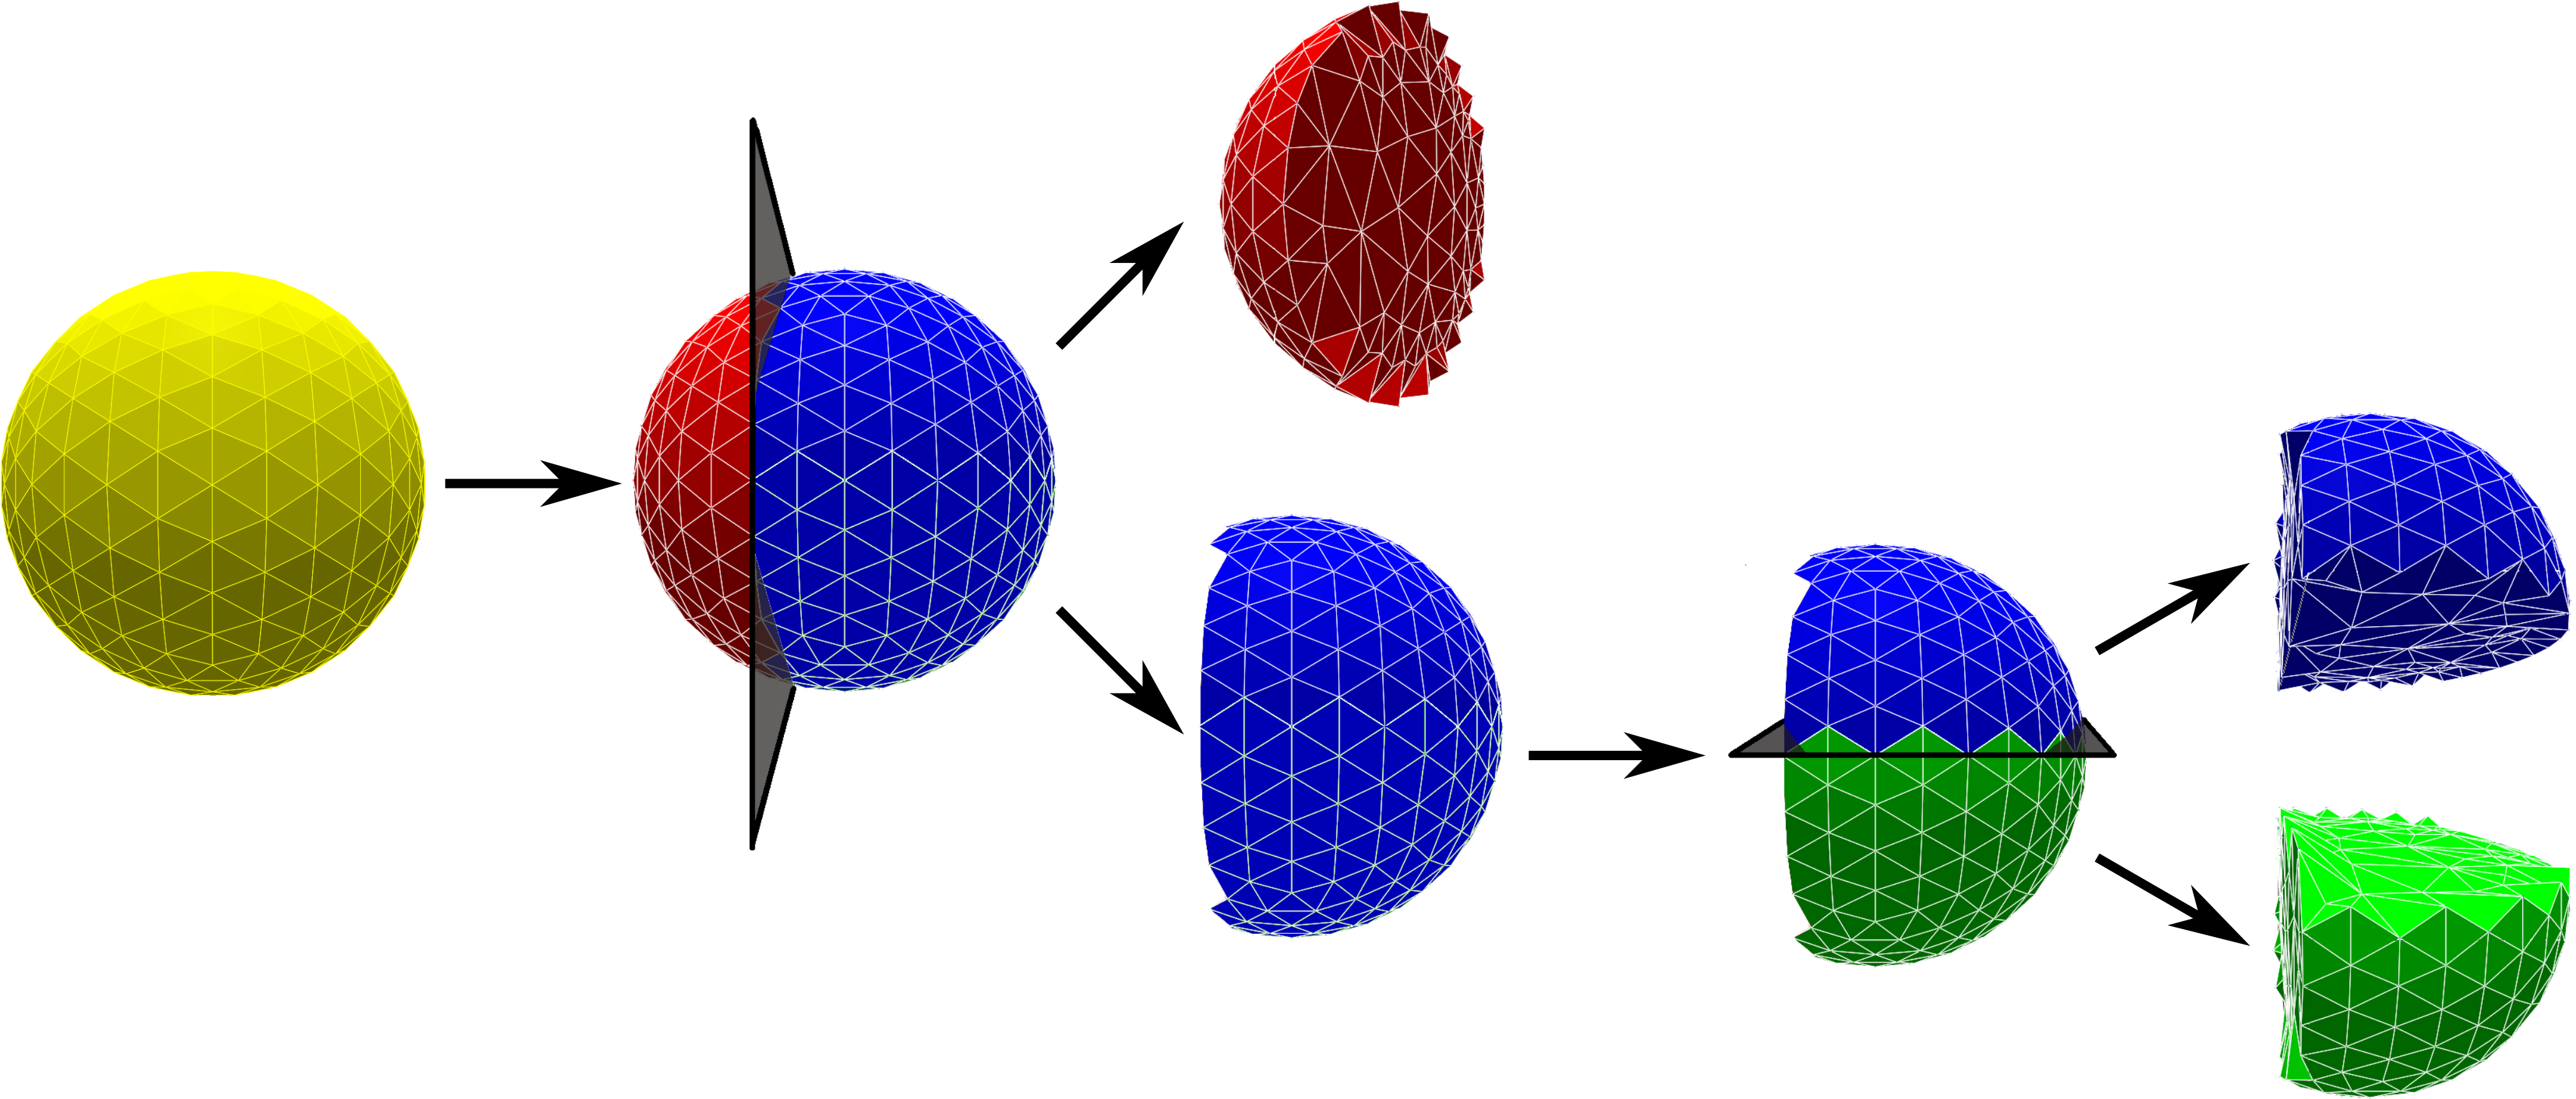
\includegraphics[width=1.0\textwidth]{fig/fluxograma_new.png}
	\caption{Visão geral da técnica paralela.}
	\label{fig:fluxograma}
\end{figure}


\section{Estimativa de Carga} 
\label{sec:Estimativa_de_Carga}

Em Computação de Alto Desempenho (CAD), a carga é uma medida da quantidade de trabalho a ser realizado em um subdomínio ou um conjunto de subdomínios. Em problemas de geração de malha, a carga está relacionada com o número de elementos que serão gerados em cada subdomínio. Portanto, a carga está relacionada com as seguintes questões que devem ser levadas em conta em sua estimativa (Figuras~\ref{fig:malha_norma_refinada} e~\ref{fig:malha_uniforme_não_uniforme}):

\begin{itemize}
	\item O nível de discretização da malha, geralmente especificado pelo usuário ou por outro software, através de parâmetros de entrada. Quanto maior a discretização da malha, maior será a carga (Figura \ref{fig:malha_norma_refinada} e \ref{fig:malha_norma_refinada_trid});

\begin{figure}[!ht]
	\centering
	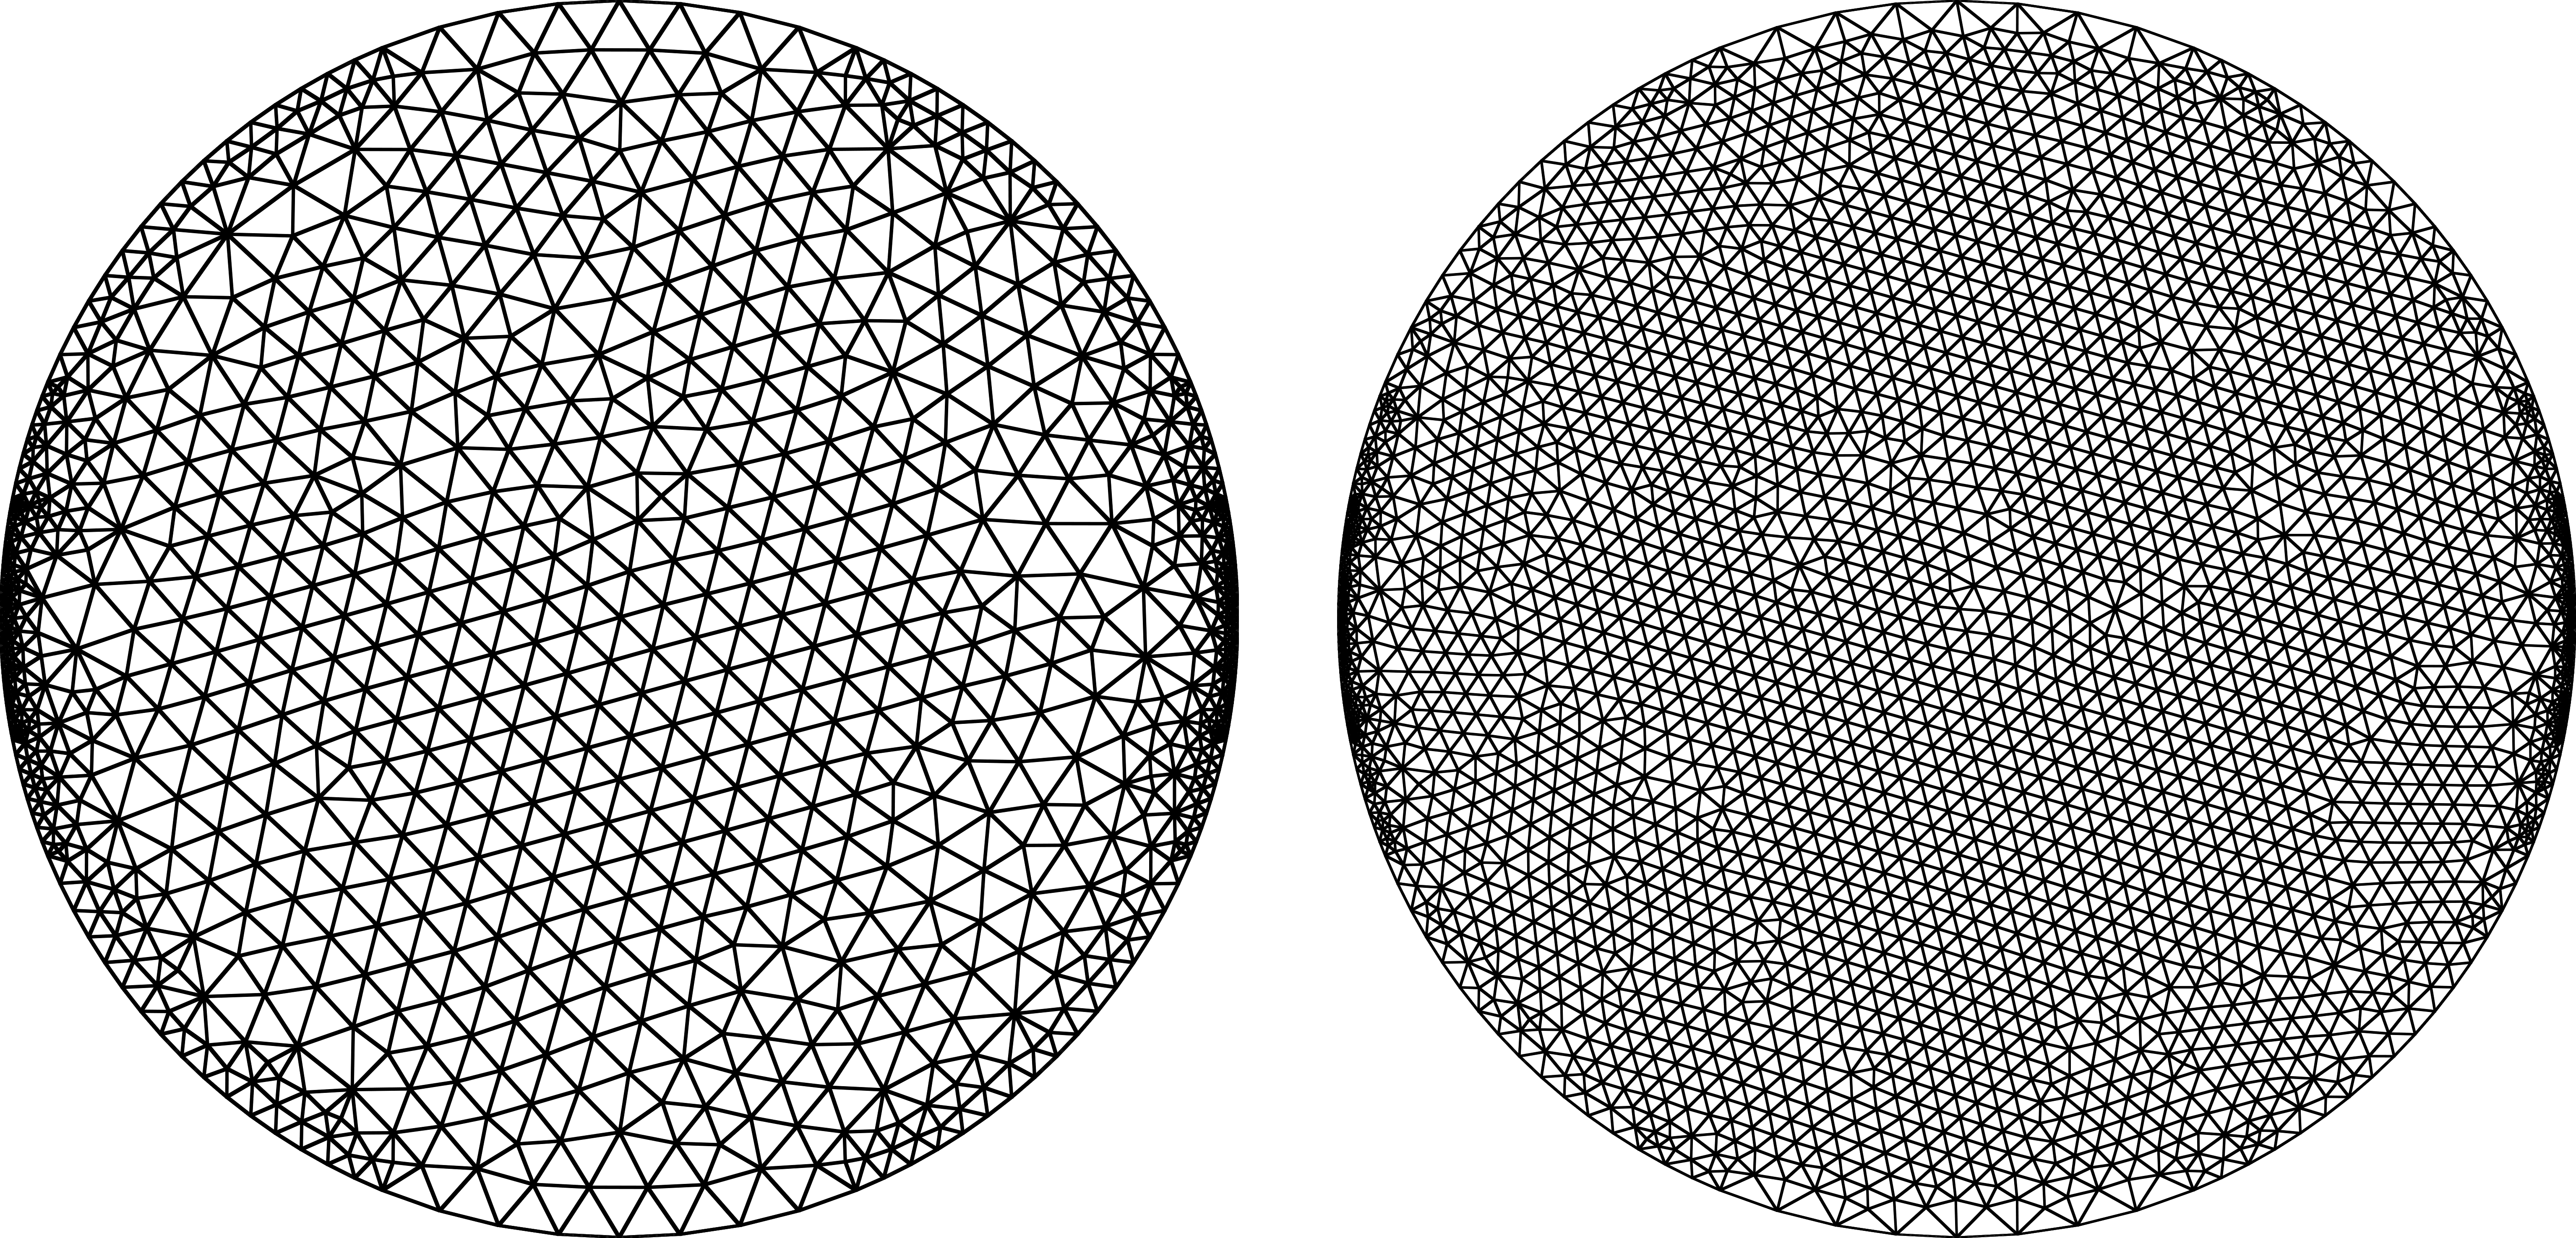
\includegraphics[width=0.9\textwidth]{fig/meshes_normal_and_refined.png}
	\caption{Estimativa de carga para o caso bidimensional: refinamento menor (esquerda) e maior (direita).}
	\label{fig:malha_norma_refinada}
\end{figure}

\begin{figure}[!ht]
	\centering
	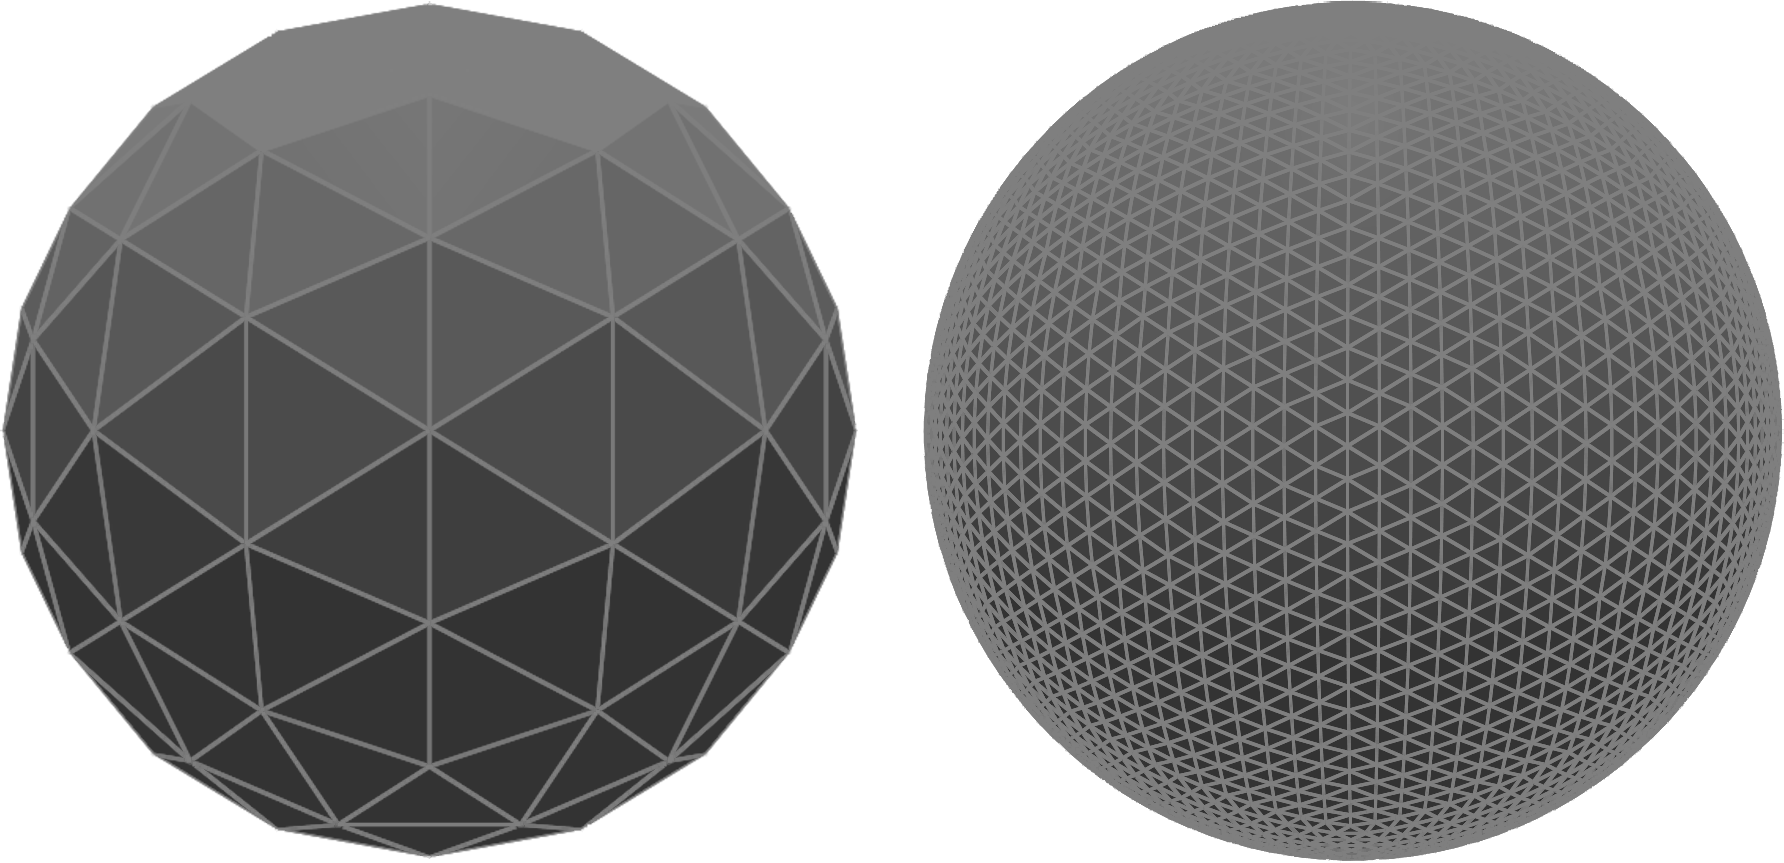
\includegraphics[width=0.9\textwidth]{fig/esferas_comp_ref.png}
	\caption{Estimativa de carga para o caso tridimensional: refinamento menor (esquerda) e maior (direita).}
	\label{fig:malha_norma_refinada_trid}
\end{figure}

	\item Em regiões com o mesmo nível de discretização, uma região maior gera mais elementos do que uma região menor. Assim, quanto maior for a região, maior será a carga (esquerda da Figura \ref{fig:malha_uniforme_não_uniforme} e \ref{fig:malha_uniforme_não_uniforme_trid});
	\item Em domínios com diferentes níveis de discretização, regiões de mesmo tamanho podem gerar um número de elementos diferente, dependendo do nível de refinamento de cada região. Assim, quanto mais refinada for a malha na região, maior será a carga(direita da Figura \ref{fig:malha_uniforme_não_uniforme} e \ref{fig:malha_uniforme_não_uniforme_trid}).
\end{itemize}


\begin{figure}[!ht]
	\centering
	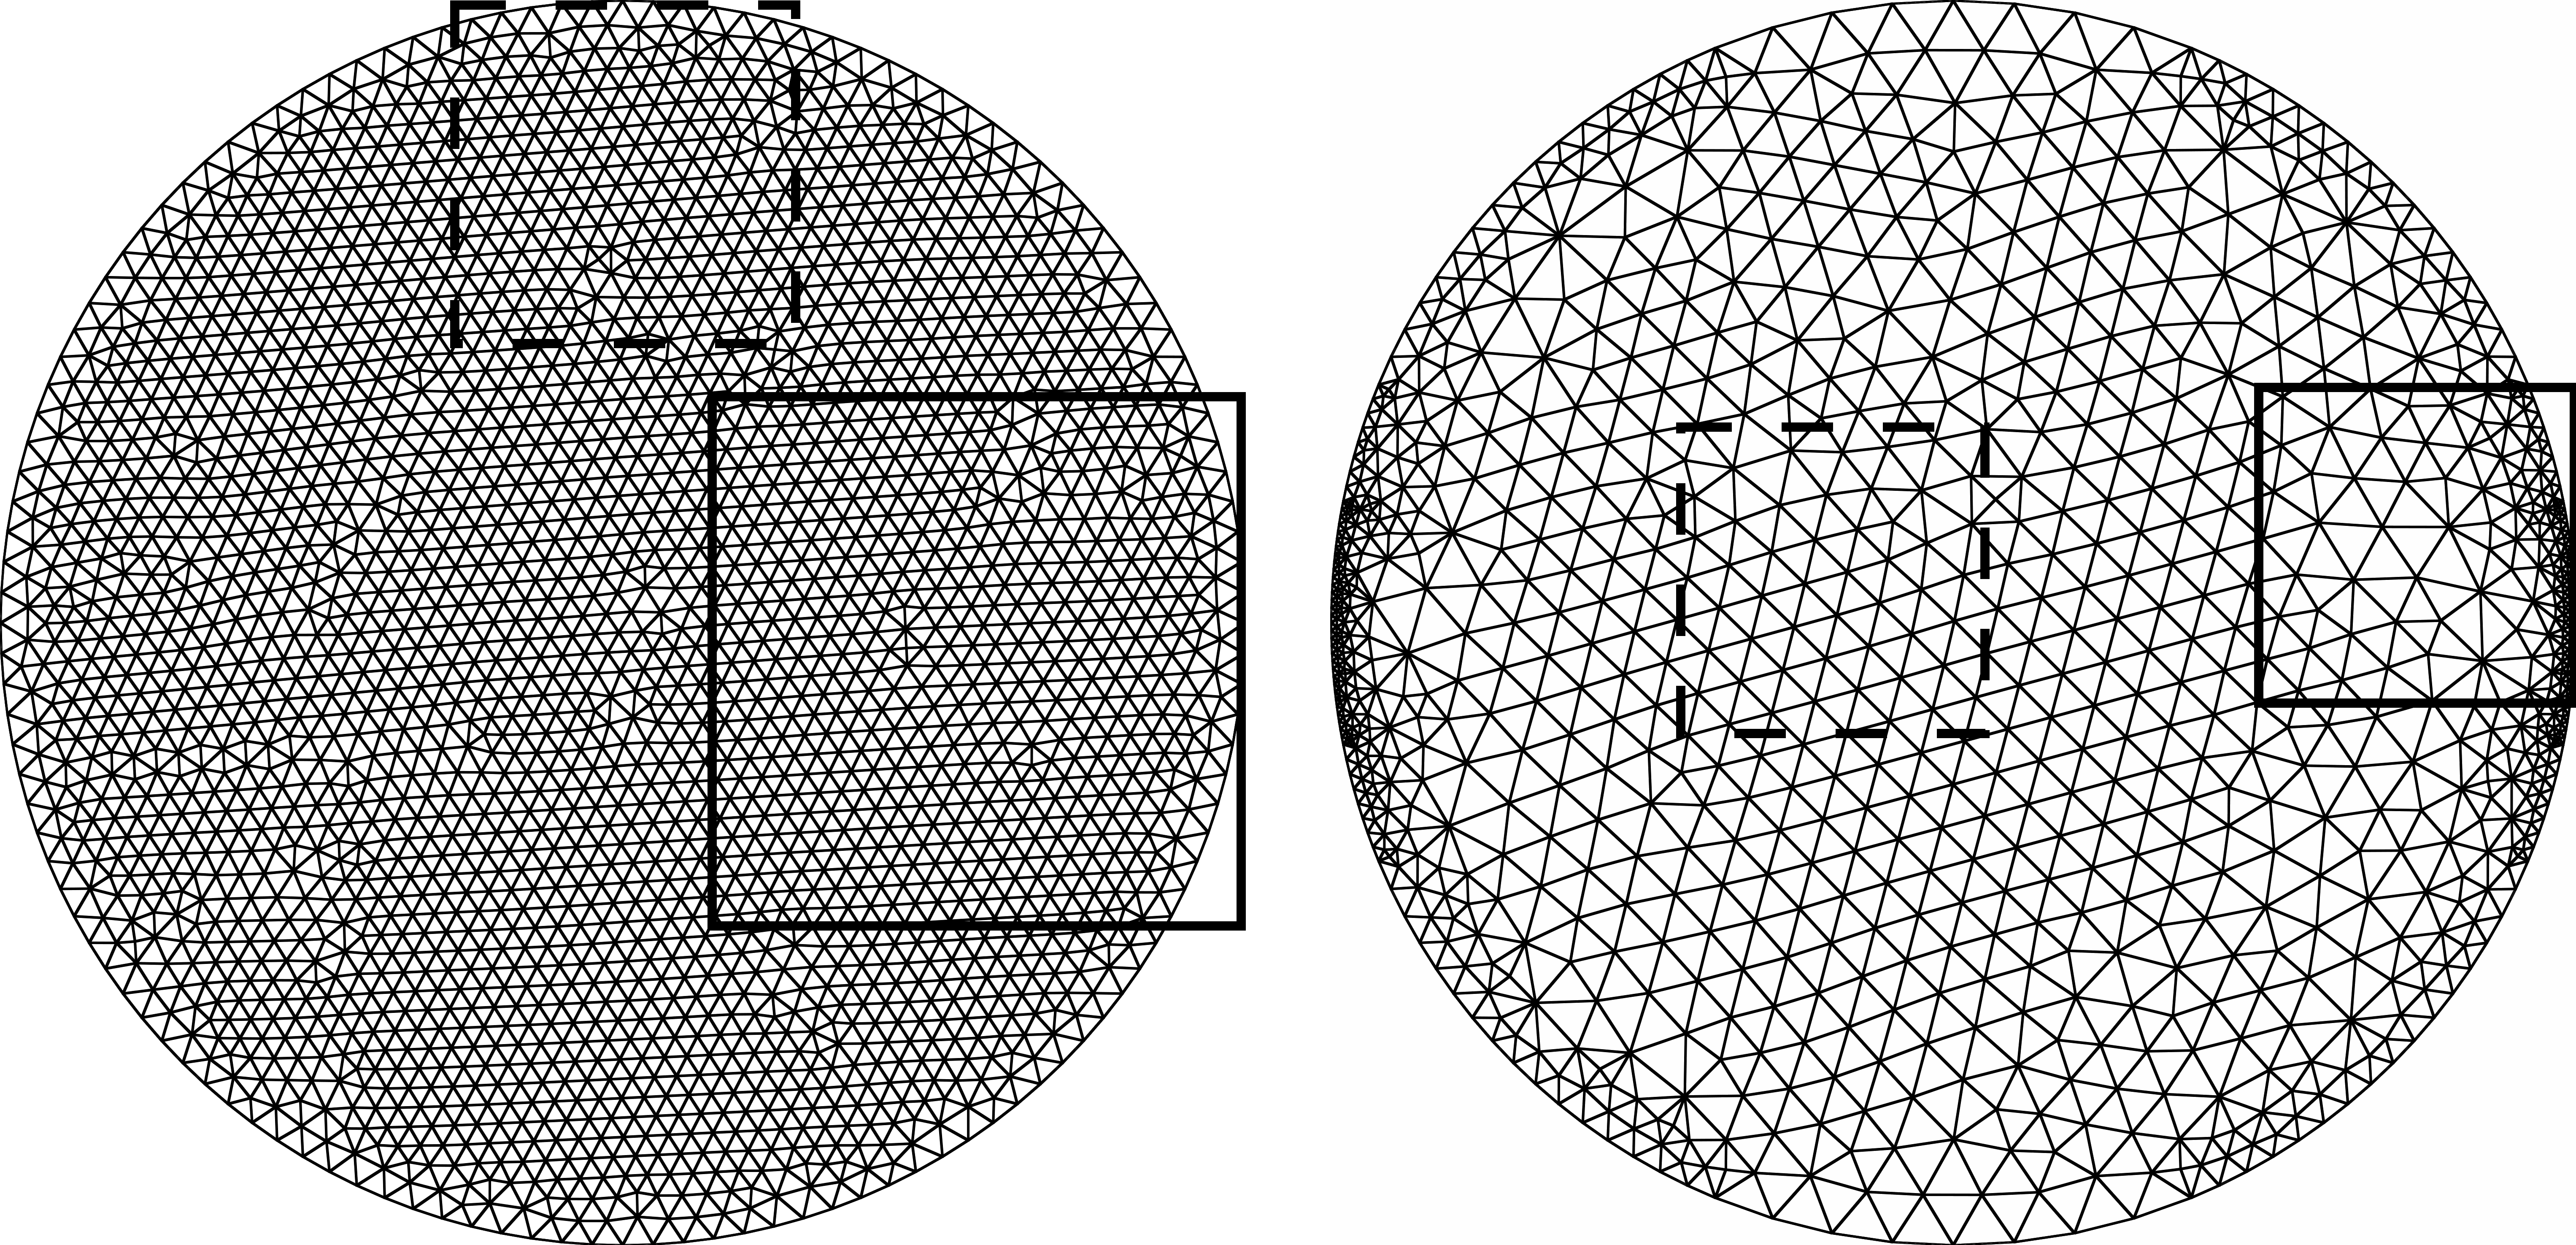
\includegraphics[width=0.9\textwidth]{fig/meshes_transition_and_uniform.png}
	\caption{Estimativa de carga para o caso bidimensional: malha uniforme (esquerda) e não-uniforme (direita).}
	\label{fig:malha_uniforme_não_uniforme}
\end{figure}

\begin{figure}[!ht]
	\centering
	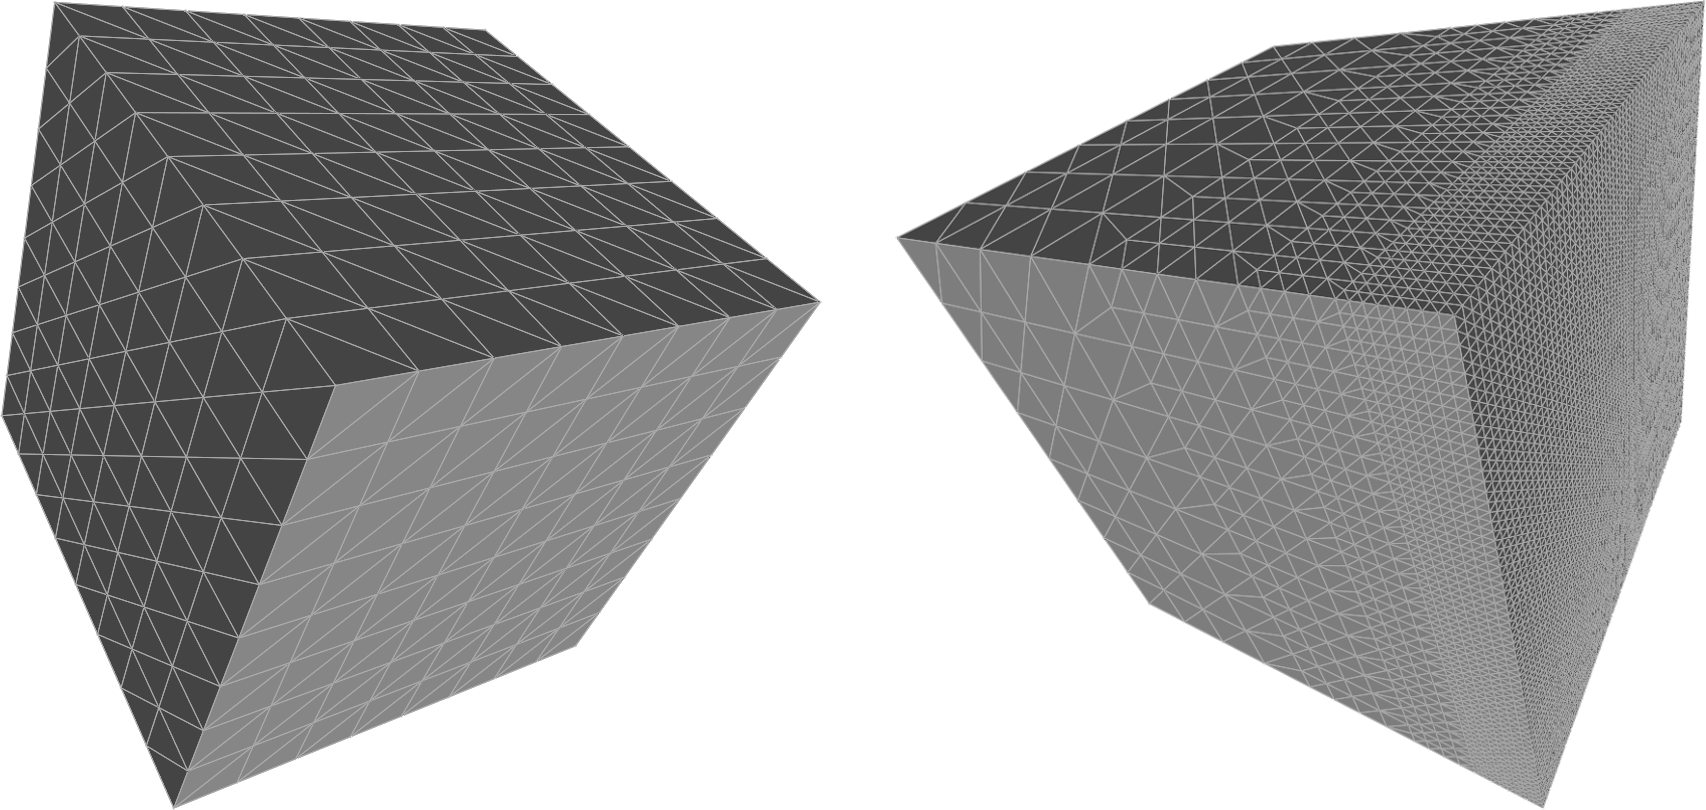
\includegraphics[width=0.9\textwidth]{fig/cubes_comp_uniform.png}
	\caption{Estimativa de carga para o caso tridimensional: faces de um cubo com malha uniforme (esquerda) e um cubo com malha não-uniforme (direita).}
	\label{fig:malha_uniforme_não_uniforme_trid}
\end{figure}

A malha da direita da Figura~\ref{fig:malha_norma_refinada} sugere uma carga maior que a malha da esquerda da mesma figura. A mesma discretização de borda foi utilizada nos dois casos. Na Figura~\ref{fig:malha_uniforme_não_uniforme}, a carga associada às regiões cercadas por linhas contínuas é maior que a carga associada às regiões cercadas por linhas tracejadas.

\subsection{Estrutura de Estimativa de Carga}

Para estimar a carga de um modelo dado como entrada é utilizado uma \textit{quadtree}, caso seja bidimensional, ou uma \textit{octree}, caso seja tridimensional. As mesmas regras de criação da \textit{quadtree} se aplicam na \textit{octree}, sendo assim, por ser mais simples de representar e entender, será explicado todo o processo usando como base a \textit{quadtree}.

A \textit{quadtree} de estimativa de carga ou \textit{quadtree} de densidade é utilizada tanto para estimar a carga como para auxiliar a geração das malhas de interface. Sua criação é iniciada com a construção de um quadrado de tamanho mínimo que engloba toda a fronteira dada como entrada (Figura \ref{fig:passo0_estimativa}); este quadrado é a célula-raiz da \textit{quadtree}. Esta \textit{quadtree} será subdividida até que todos os pontos médios das arestas da entrada estejam dentro de uma célula da \textit{quadtree} de densidade (Figura \ref{fig:passo1_estimativa}). O tamanho destas células tem de ser menor que o comprimento da aresta à qual o ponto médio pertence, multiplicada por uma constante. Essa constante tem valor $\sqrt{3}/2$, que equivale a 0,85, que é uma aproximação da altura de um triângulo equilátero. Para o caso tridimensional esta constante tem valor $\sqrt{6}/3$, que equivale a 0,81, que é uma aproximação da altura de um tetraedro regular.

Dois refinamentos são então aplicados. O primeiro é para garantir que todas as células da \textit{quadtree} de densidade não sejam maiores que a maior célula que contém um ponto médio da borda de entrada (Figura \ref{fig:passo2_estimativa}). Com esse refinamento é garantido um tamanho máximo para as células de acordo com as arestas da fronteira. Assim, os elementos que serão gerados no interior do domínio terão proporções iguais aos da borda. 

O segundo refinamento, também conhecido na literatura como refinamento 2:1, é para garantir que a diferença de níveis da \textit{quadtree} não seja maior que 2 para células vizinhas (que compartilham um lado), como mostrado na Figura \ref{fig:passo3_estimativa}. Este refinamento é feito para garantir uma transição suave entre elementos grandes e pequenos. Mais detalhes da construção desta \textit{quadtree} podem ser encontrados em \cite{bib:Miranda99} (a construção de sua versão tridimensional, uma \textit{octree}, pode ser encontrada em~\cite{bib:Cavalcante-Neto01}).


    \begin{figure}[ht]
    	\centering
    	\subfloat[Fronteira de entrada juntamente com sua caixa delimitadora (em vermelho).]
    	{\label{fig:passo0_estimativa}
    		\begin{minipage}[c]{0.4\textwidth}{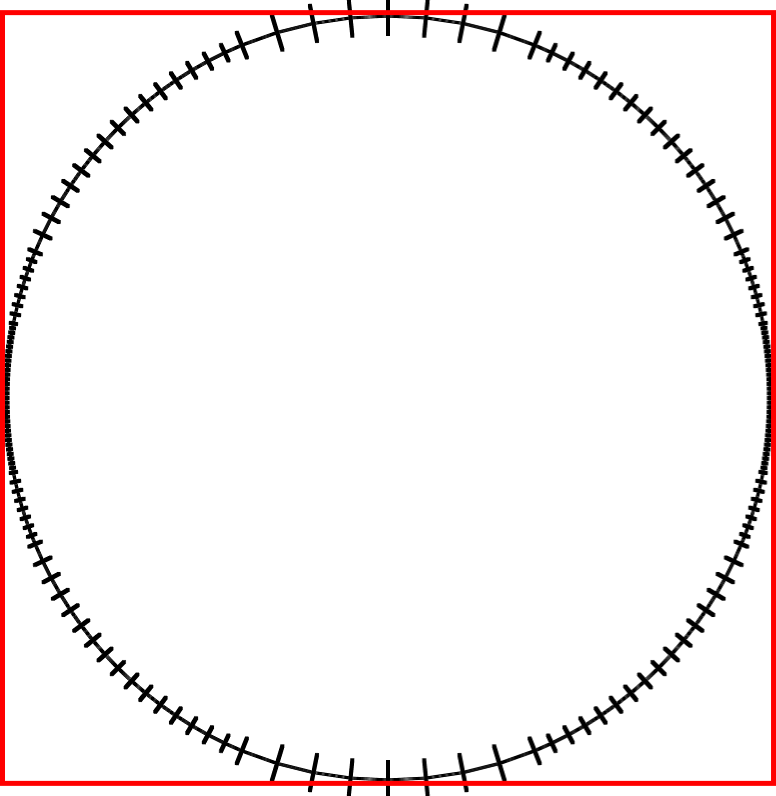
\includegraphics[width=\textwidth]{fig/passo0.png}}\end{minipage}
    	}
    	\qquad
    	\subfloat[\textit{Quadtree} de densidade inicialmente gerada.]
    	{\label{fig:passo1_estimativa}
    		\begin{minipage}[c]{0.4\textwidth}{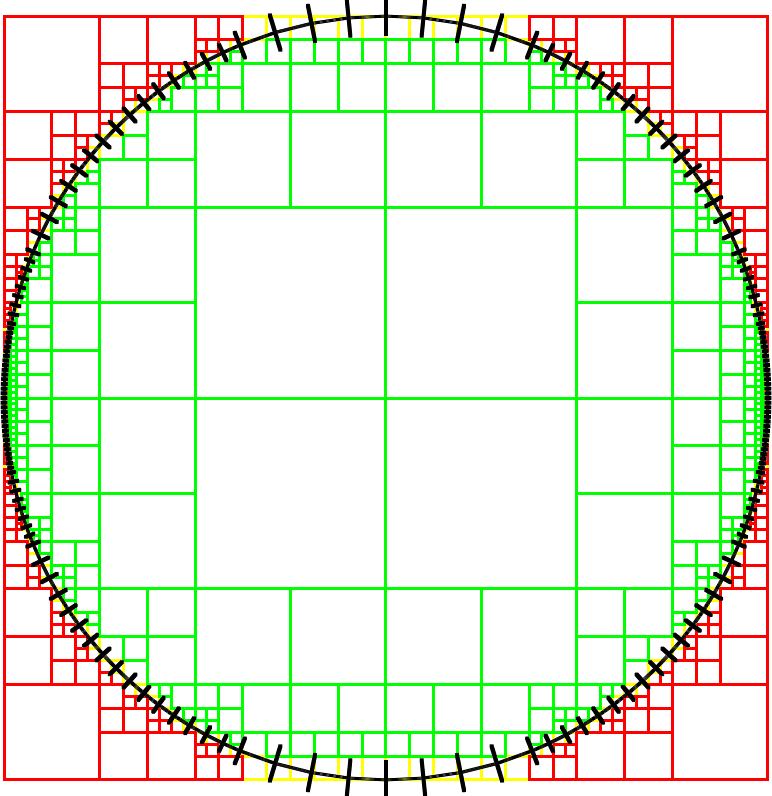
\includegraphics[width=\textwidth]{fig/passo1.png}}\end{minipage}
    	}
    	
    	\subfloat[Primeiro refinamento na \textit{quadtree} de densidade.]
    	{\label{fig:passo2_estimativa}
    		\begin{minipage}[c]{0.4\textwidth}{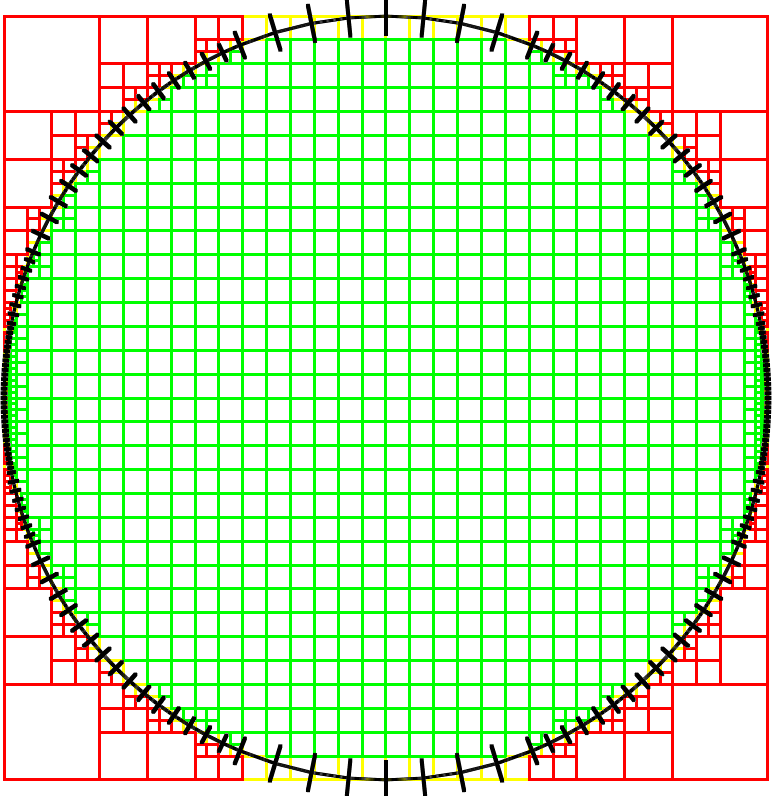
\includegraphics[width=\textwidth]{fig/passo2.png}}\end{minipage}
    	}    
    	\qquad
    	\subfloat[Segundo refinamento na \textit{quadtree} de densidade.]
    	{\label{fig:passo3_estimativa}
    		\begin{minipage}[c]{0.4\textwidth}{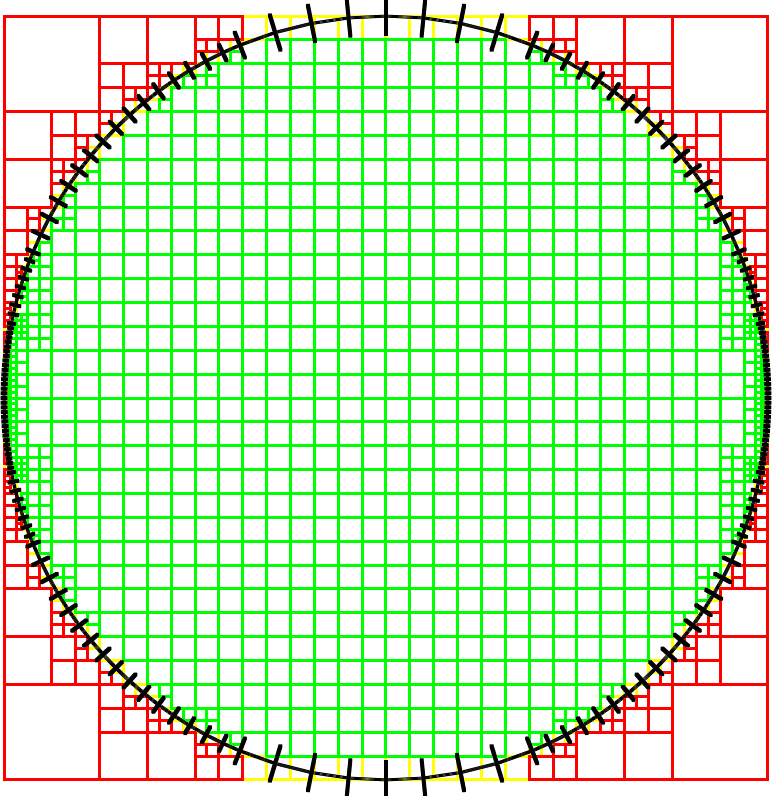
\includegraphics[width=\textwidth]{fig/passo3.png}}\end{minipage}
    	}
    	\caption{Passos da geração da \textit{quadtree} de densidade.}
    	\label{fig:passos_estimativa}
    \end{figure}


\subsection{Classificação das Células}

Uma classificação das células da \textit{quadtree} de densidade contribui para otimizar buscas e para evitar o desperdício de memória. Pode-se classificar uma célula como interna (caso a célula esteja totalmente interna ao domínio), externa (caso a célula esteja totalmente externa ao domínio) ou sobre a fronteira do domínio (caso a célula faça interseção com alguma aresta ou vértice do domínio). O algoritmo de classificação é mostrado em \cite{bib:Freitas10}. A Figura \ref{fig:classificacao} mostra as células de uma \textit{quadtree} de densidade classificadas para um dado domínio circular, onde as cores atribuídas às células indicam a sua classificação (células verdes - dentro do domínio, células vermelhas - fora do domínio, células amarelas - sobre a fronteira).

\begin{figure}[!ht]
	\centering
	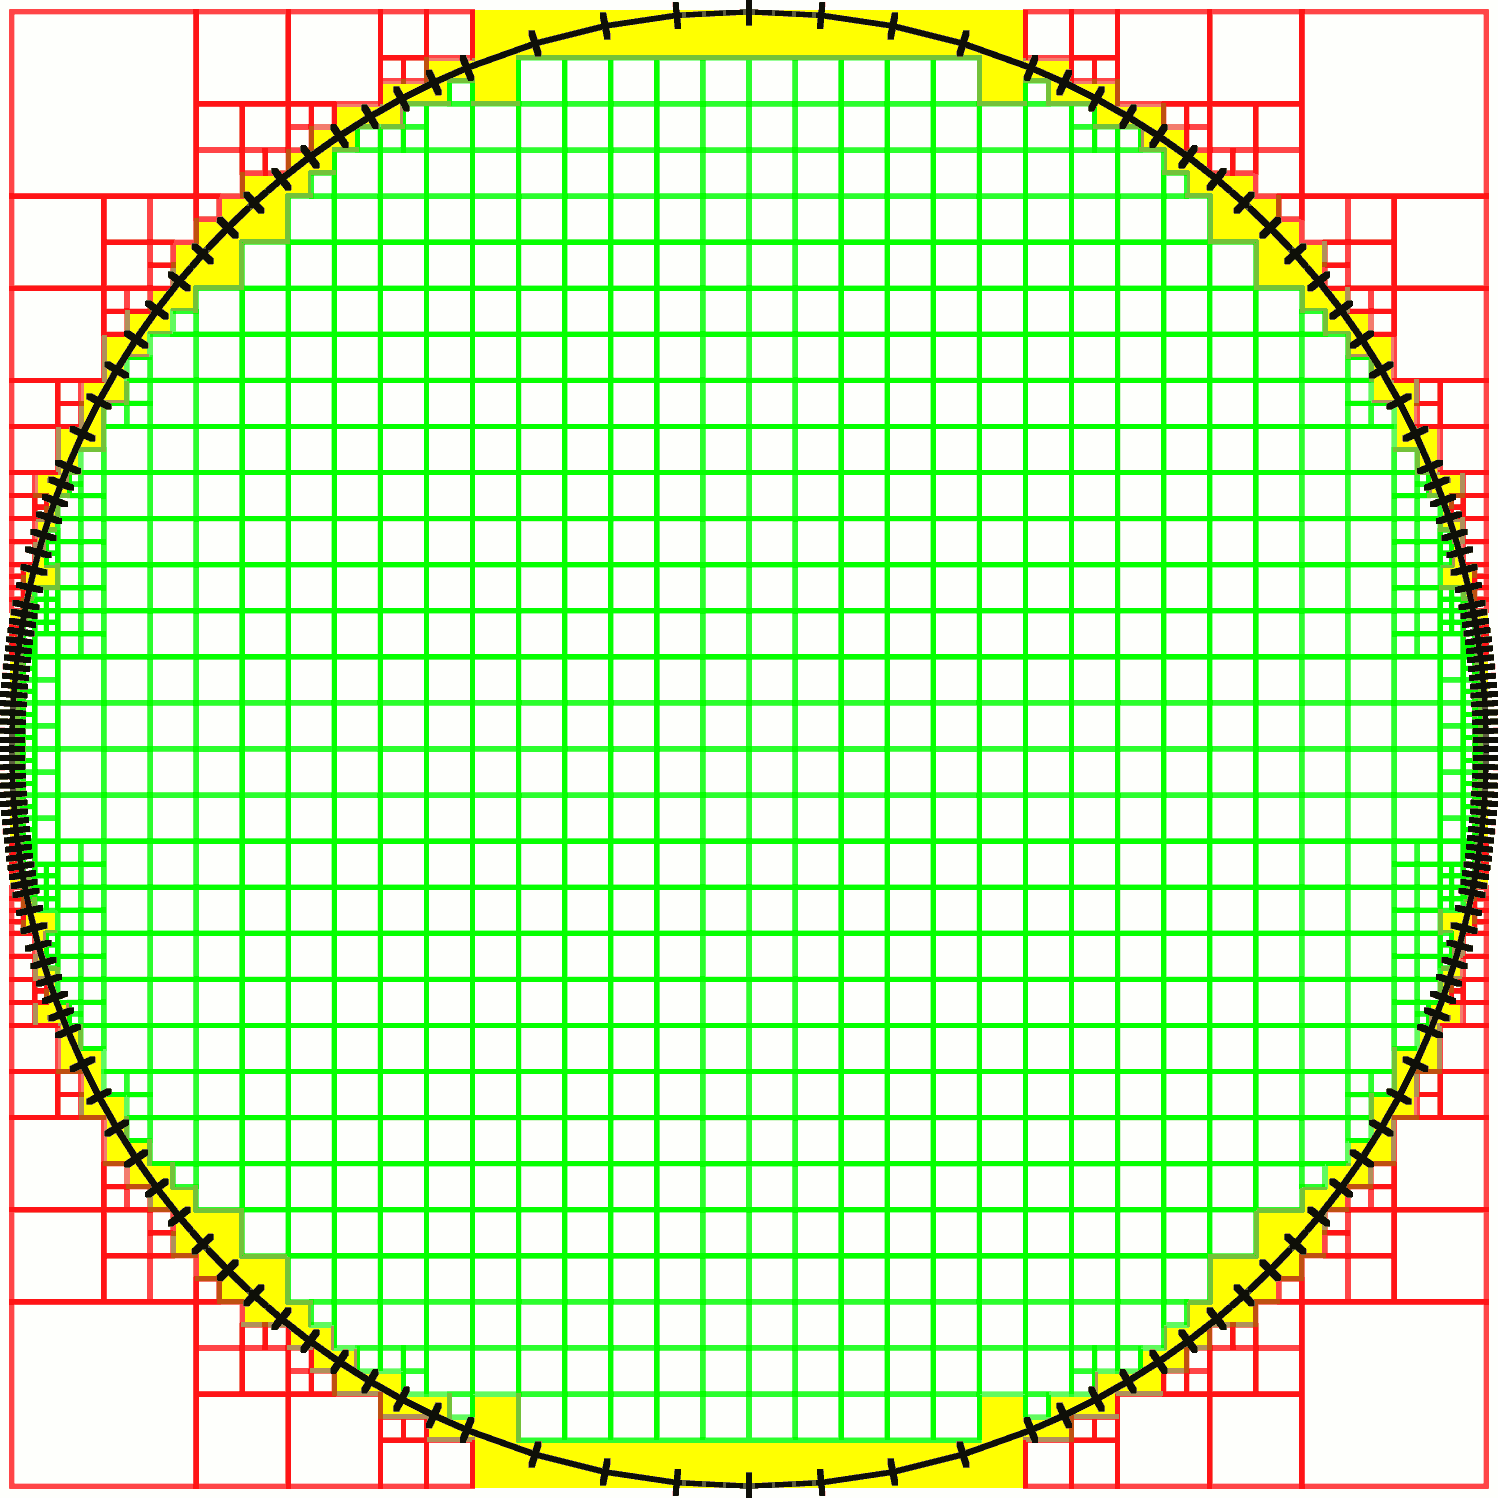
\includegraphics[width=0.4\textwidth]{fig/classificacao.png}
	\caption{\textit{Quadtree} de densidade com as células devidamente classificadas (células verdes - dentro do domínio, células vermelhas - fora do domínio, células amarelas - sobre a fronteira).}
	\label{fig:classificacao}
\end{figure}


\subsection{Cálculo da Carga}

A \textit{quadtree} de densidade é utilizada para fazer uma estimativa da carga neste trabalho. Com a sua construção é possível ter noção do tamanho dos elementos pertencentes ao domínio do objeto. Assim, uma ideia geral sobre a malha desejada é conhecida desde o início. A classificação das células folhas da \textit{quadtree} de densidade é utilizada para selecionar apenas as células que não estão fora do domínio de entrada, ou seja, as células que estão no interior do domínio e as que interceptam a borda (células verdes e amarelas na Figura \ref{fig:classificacao}). A quantidade dessas folhas não externas é considerada como a carga total para este domínio.

\section{Decomposição do Domínio}\label{sec:Decomposicao_dominio}

A técnica proposta neste trabalho tem apenas um pré-requisito quanto à estrutura de decomposição espacial para particionar o domínio dado como entrada. A estrutura de decomposição utilizada deve gerar regiões que sejam paralelas às células da \textit{quadtree} de densidade. Estruturas baseadas em árvore como \textit{quadtree}, \textit{octree}, BSP (\textit{Binary Space Partition}) e \textit{Kd-tree} (\textit{k-dimensional tree}) geram regiões que possibilitam a perfeita execução do algoritmo de geração dos subdomínios.

Essa restrição tem a finalidade de facilitar a estimativa de carga dos novos subdomínios que serão criados após o corte. Classificar uma célula dessas estruturas espaciais como interna ou externa a um plano de partição ou corte é muito mais simples e exato que computar interseções entre eles. Calcular interseções da partição com as células da estrutura de estimativa de carga para descobrir a fração de carga que estaria interna ou externa a partição seria pesado computacionalmente.

Vale lembrar que para um bom particionamento é preciso uma boa estimativa de carga e, para se obter uma malha de boa qualidade, depende de um bom particionamento do domínio. Esta seção descreve como é feita a criação de uma BSP para decompor a entrada. Dentre todas as estruturas de dados testada, a BSP (\textit{Binary Space Partition}), é a que da mais liberdade na criação das partições


\subsection{Decomposição Utilizando BSP}

Uma excelente estrutura de particionamento espacial é a BSP, aqui chamada de BSP de decomposição, tendo a sua criação guiada pela estrutura de estimativa de carga descrita anteriormente na Seção~\ref{sec:Estimativa_de_Carga}. A utilização desta estrutura foi baseada no trabalho de \cite{bib:RepMarkos13}, onde mais detalhes da construção e implementação podem ser encontrados nele. A BSP de decomposição pode ser construída de diversas formas, dependendo apenas do critério de subdivisão:


\begin{itemize}
	\item Subdivisão baseada na carga. Cada célula folha não pode ter uma carga maior que a carga média;
	\item Subdivisão baseada na diferença de carga total de cada as partições (Figura \ref{fig:bsp_decomposition_passos}); e 
	\item Subdivisão baseada no eixo mediano.
\end{itemize}


\begin{figure}[!ht]
	\centering
	\subfloat[Primeiro corte criado com pesos 5 para cada lado.]
	{\label{fig:bsp_decomposition_passos1}
		\begin{minipage}[c]{0.3\textwidth}{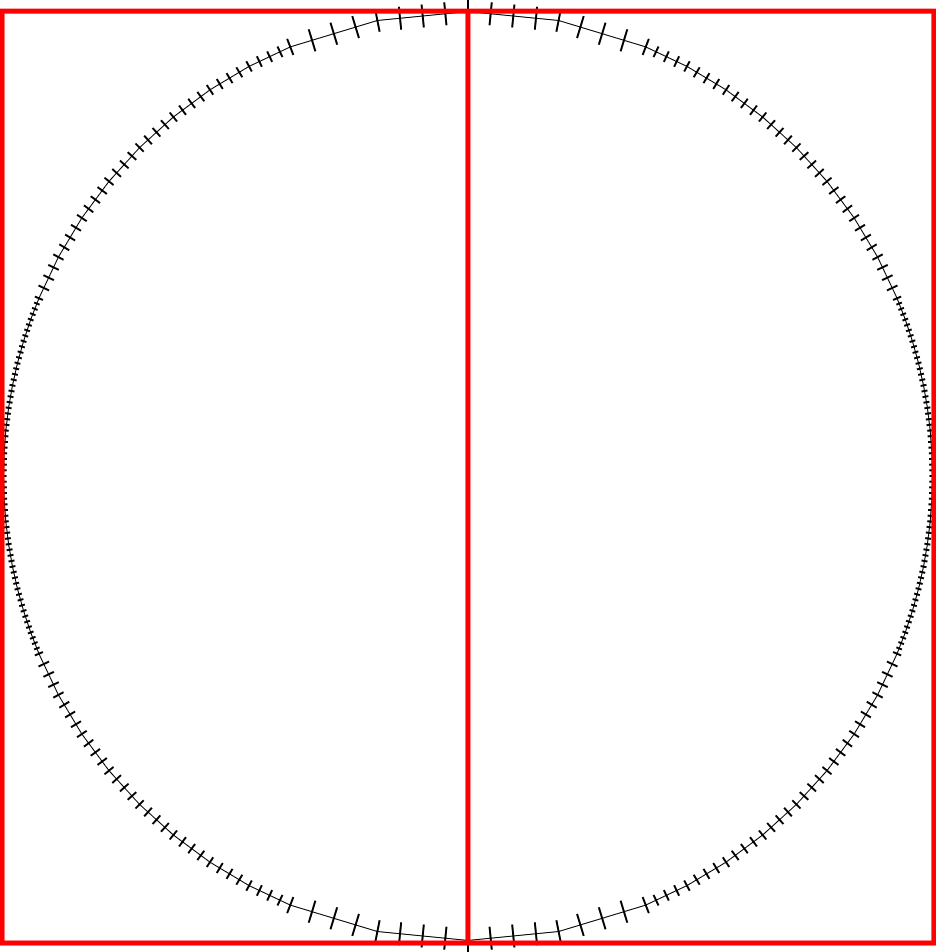
\includegraphics[width=\textwidth]{fig/bsp_passo1.png}}\end{minipage}
	}
	\qquad
	\subfloat[Segundo corte criado com pesos 2 e 3 para cada lado.]
	{\label{fig:bsp_decomposition_passos2}
		\begin{minipage}[c]{0.3\textwidth}{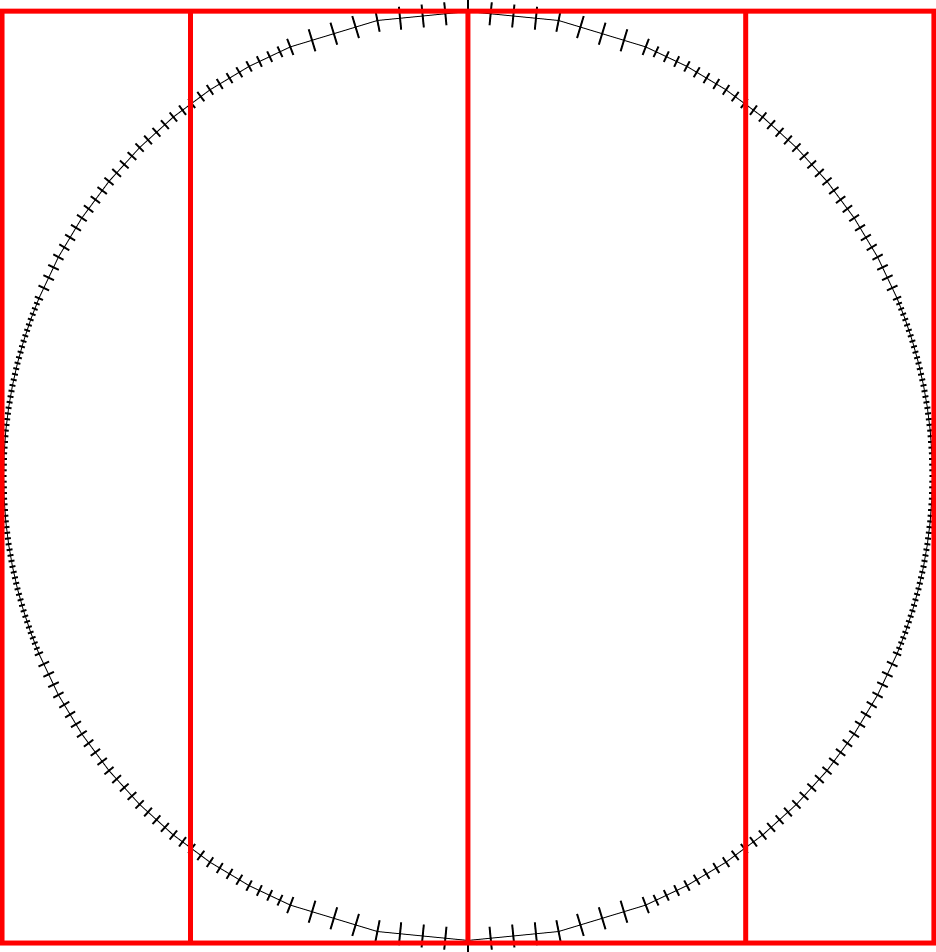
\includegraphics[width=\textwidth]{fig/bsp_passo2.png}}\end{minipage}
	}
	
	\subfloat[Terceiro corte criado gerando dois subdomínios.]
	{\label{fig:bsp_decomposition_passos3}
		\begin{minipage}[c]{0.3\textwidth}{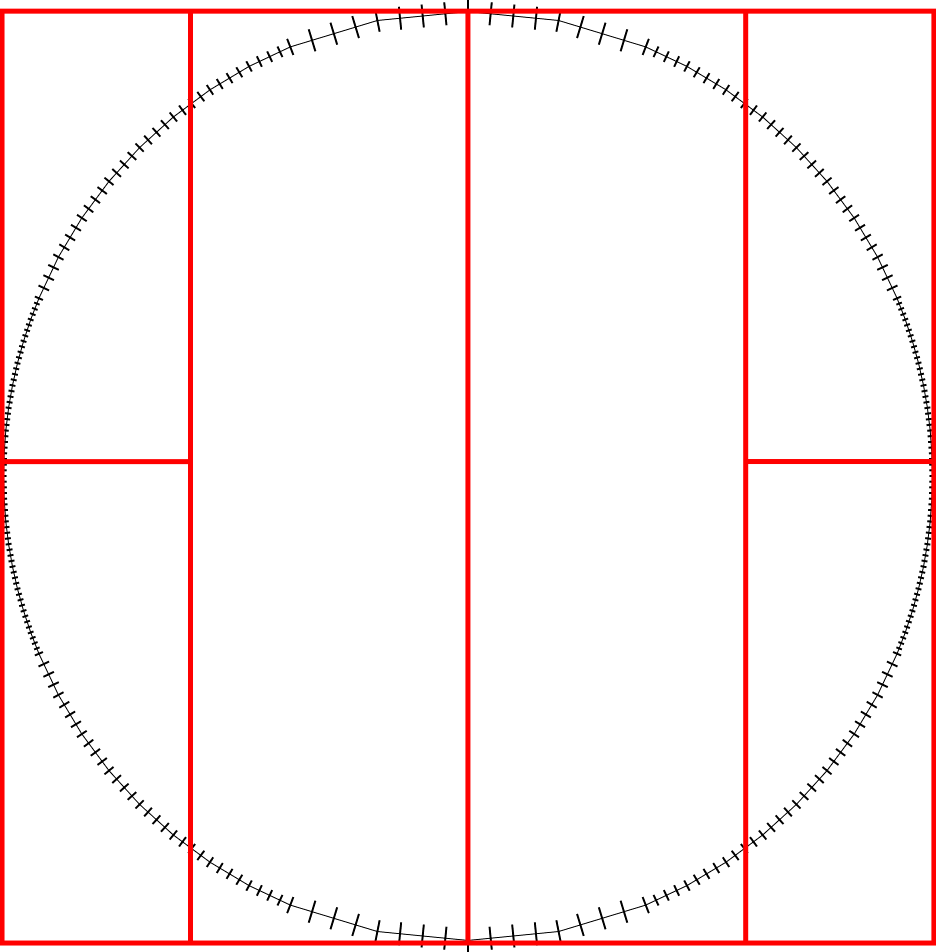
\includegraphics[width=\textwidth]{fig/bsp_passo3.png}}\end{minipage}
	}
	\qquad
	\subfloat[Último corte criado finalizando os 10 subdomínios.]
	{\label{fig:bsp_decomposition_passos4}
		\begin{minipage}[c]{0.3\textwidth}{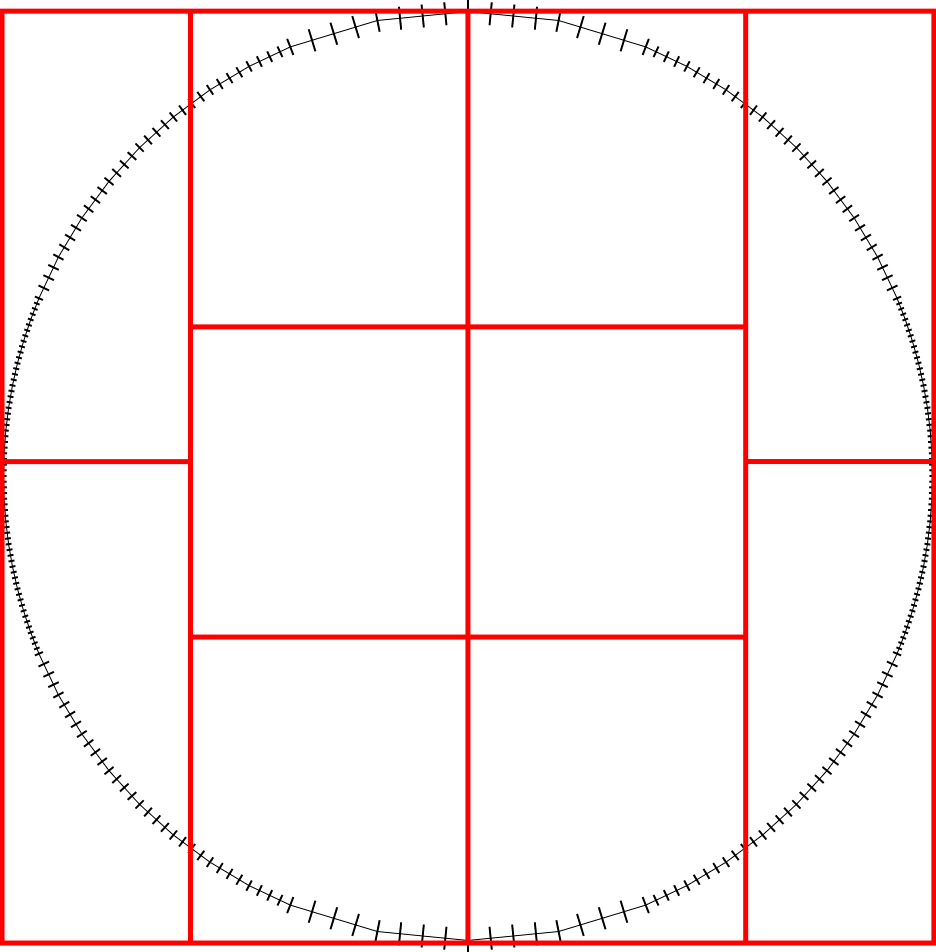
\includegraphics[width=\textwidth]{fig/bsp_passo4.png}}\end{minipage}
	}    
	\caption{Exemplo da criação de uma BSP bidimensional para 10 processadores baseada na diferença de carga.}
	\label{fig:bsp_decomposition_passos}
\end{figure}    


As principais vantagens da utilização de uma BSP são a quantidade de subdivisões realizadas e a liberdade que a BSP tem de subdividir o domínio em regiões de diferentes tamanhos. A possibilidade de gerar a quantidade de regiões que sejam necessárias com diferentes tamanhos torna o particionamento muito mais preciso. A Figura \ref{fig:bsp_decomposition_passos} mostra o passo a passo da criação de uma BSP de particionamento feita para dez processadores, ou seja, dez subdomínios foram criados.

A forma mais eficiente para gerar a BSP de decomposição é a que faz a carga associada com cada uma das folhas ser menor que uma carga máxima pré-definida $L/P$, sendo $L$ a carga total da entrada e $P$ a quantidade de processadores disponíveis. Com a BSP, é possível obter $N=P$, sendo $N$ a quantidade de subdomínios criados, com uma carga muito próxima a $L/P$ para cada $P$.

Inicia-se a BSP de decomposição com sua raiz definida como um quadrado, para o caso bidimensional, ou um cubo, para o caso tridimensional, envolvendo o domínio. A subdivisão é feita posicionando a partição no centro geométrico dessa célula, no eixo X. Se esta partição obtiver cargas iguais para os dois filhos, essa partição será a melhor para o eixo X. Caso contrário, seleciona-se a célula mais pesada e reposiciona-se o plano de partição para a metade dessa célula, no mesmo eixo. Este procedimento é feito recursivamente até que as cargas dos dois subdomínios sejam iguais ou, quando atinge-se uma célula-folha da estrutura de estimativa, \textit{quadtree} para o caso bidimensional ou \textit{octree} para o caso tridimensional, ou seja, é impossível subdividir esta célula.

Esse procedimento é realizado em todos os eixos e ao final é selecionado o particionamento no eixo que melhor divide a carga nas duas novas células criadas. A Figura \ref{fig:passos_decomposicao_BSP} mostra o passo a passo da seleção da melhor subdivisão para o eixo X. Com essa subdivisão no eixo X, a diferença alcançada é de quatro (Figura \ref{fig:bsp_3}); porém, fazendo a decomposição no eixo Y a diferença seria de zero. O particionamento selecionado vai ser o que obtiver a menor diferença, sendo assim, para o exemplo da Figura \ref{fig:bsp_3}, o particionamento selecionado seria o do Y.


\begin{figure}[ht]
	\centering
	\subfloat[\textit{Quadtree} de estimativa de carga. Carga total: 52. Carga ideal de cada subdomínio: 26.]
	{\label{fig:bsp_0}
		\begin{minipage}[c]{0.3\textwidth}{
\includegraphics[width=\textwidth]{fig/bsp_0.png}}\end{minipage}
	}
	\qquad
	\subfloat[Posição inicial do plano de partição (em vermelho). Cargas dos subdomínios: 32 e 20. Diferença: 12.]
	{\label{fig:bsp_1}
		\begin{minipage}[c]{0.3\textwidth}{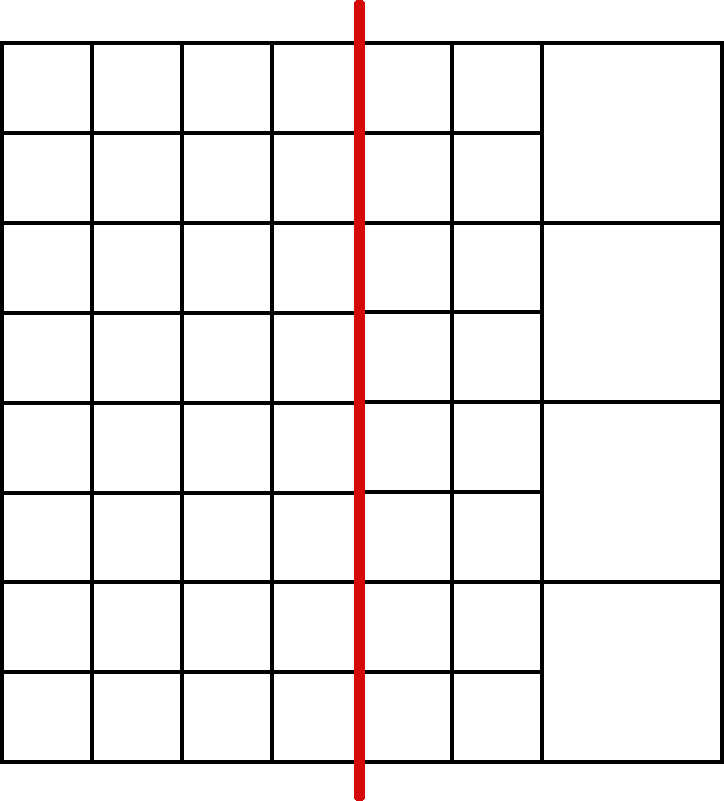
\includegraphics[width=\textwidth]{fig/bsp_1.png}}\end{minipage}
	}
	
	\subfloat[Deslocamento do plano de partição para o próximo nível da esquerda. Cargas dos subdomínios: 16 e 36. Diferença: 20.]
	{\label{fig:bsp_2}
		\begin{minipage}[c]{0.3\textwidth}{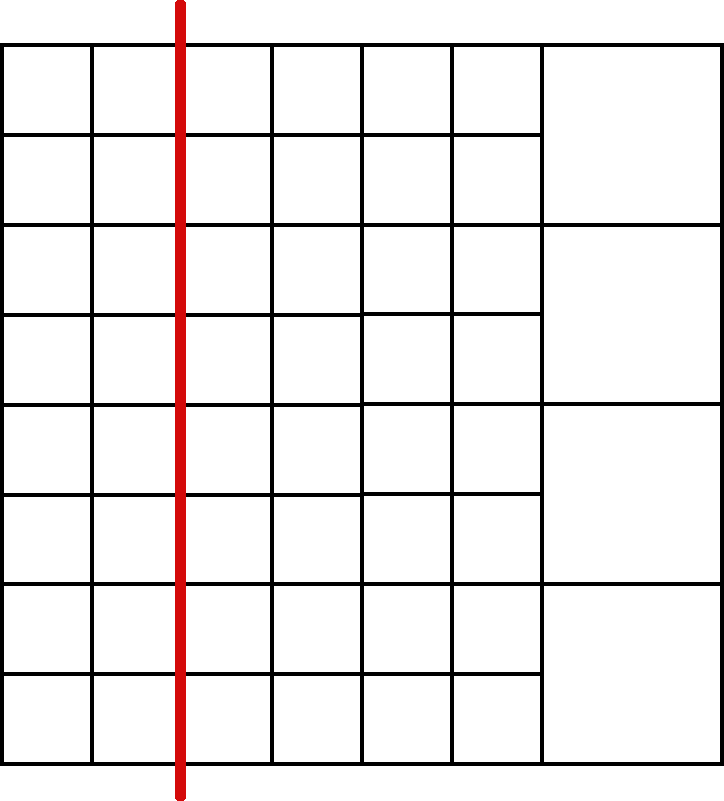
\includegraphics[width=\textwidth]{fig/bsp_2.png}}\end{minipage}
	}    
	\qquad
	\subfloat[Deslocamento do plano de partição para o próximo nível da direita. Cargas dos subdomínios: 24 e 28. Diferença: 4.]
	{\label{fig:bsp_3}
		\begin{minipage}[c]{0.3\textwidth}{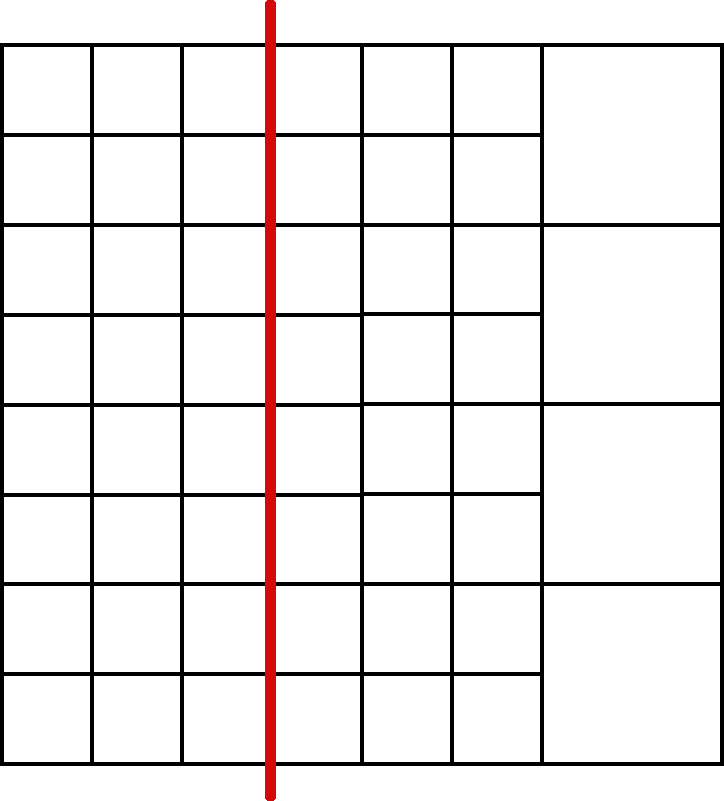
\includegraphics[width=\textwidth]{fig/bsp_3.png}}\end{minipage}
	}
	\caption{Passos de uma decomposição bidimensional de um domínio por BSP no eixo X para dois processadores, buscando a diferença mínima de carga total.}
	\label{fig:passos_decomposicao_BSP}
\end{figure}


Nos casos que o número de partições desejado seja ímpar, é aplicado um valor para indicar que a carga de uma região deve ser proporcional a $X$ vezes a de outra região. Com a aplicação desses pesos é garantido que, para qualquer quantidade de partições desejada, a BSP irá encontrar o melhor corte que dividirá a carga entre as partições. A Figura \ref{fig:circunferencia_cortejunto} mostra o processo de particionamento em uma circunferência para três regiões.

\begin{figure}[!ht]
	\centering
	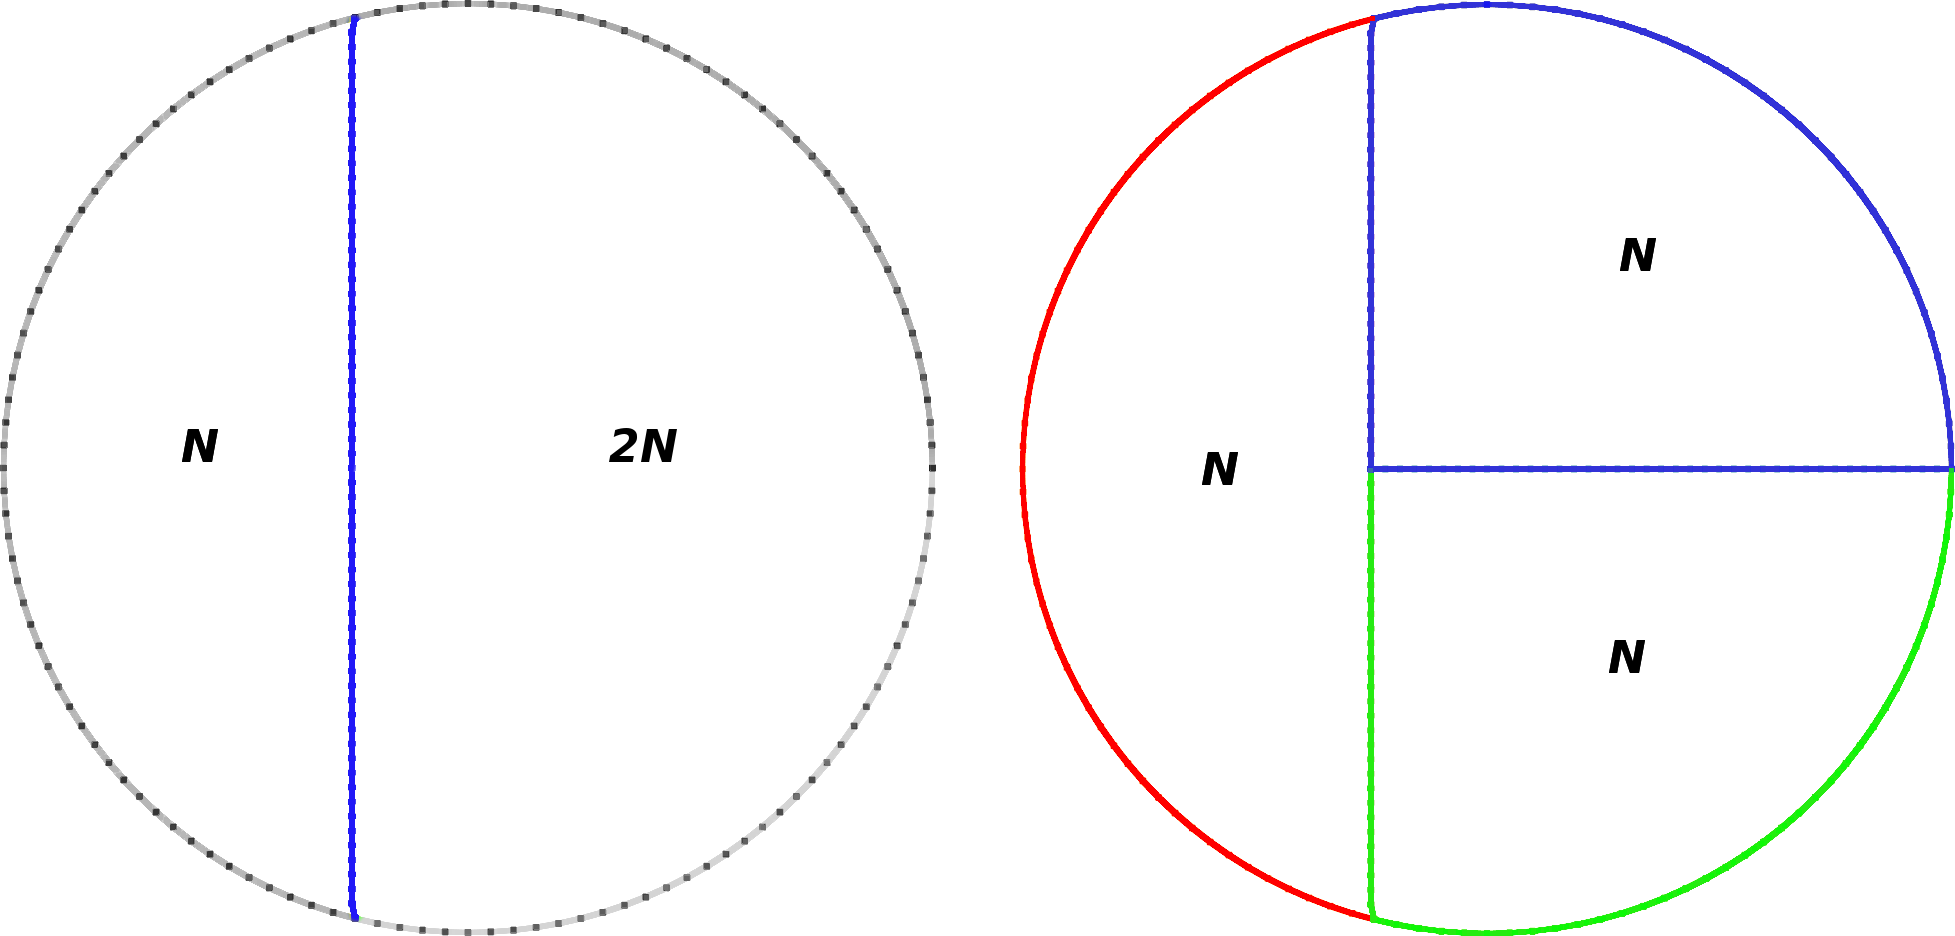
\includegraphics[width=0.7\textwidth]{fig/circunferencia_cortejunto.png}
	\caption{Proporção 2:1 é aplicada fazendo um lado ter duas vezes mais carga que o outro (lado esquerdo). Resultado final é apresentado no lado esquerdo.}
	\label{fig:circunferencia_cortejunto}
\end{figure}

\section{Interfaces dos Subdomínios}

Na geração das interfaces dos subdomínios, é necessário ter a estrutura de estimativa de carga ( uma \textit{quadtree} no caso bidimensional e uma \textit{octree} no caso tridimensional) e a estrutura de particionamento devidamente criadas (a BSP). Qualquer outra estrutura de decomposição espacial que gere regiões paralelas aos eixos pode ser utilizada nesta técnica de geração de subdomínios. 

Para construir a interface dos subdomínios é necessário possuir uma grade de suporte e os elementos do modelo de entrada em que a partição faz interseção. A grade de suporte irá guiar a criação dos elementos da interface, sendo ela responsável pelo tamanho e posicionamento dos mesmos. Os elementos do modelo que fazem interseção com a partição são necessários para fazer a junção da interface com o modelo, de tal modo que ao final não exista nenhum buraco na interface.

\subsection{Grade de Suporte}
\label{sec:Grade_Suporte}

Para cada corte da estrutura de particionamento é feita a interseção com as células folhas da estrutura de estimativa de carga (Figura \ref{fig:celulas_selecionadas2d_tree} para o caso bidimensional e Figura \ref{fig:celulas_selecionadas3d_tree} para o caso tridimensional). Como resultado dessa interseção, é obtido um conjunto de células da estrutura de estimativa de carga que cruzam ou apenas tangenciam a partição que se deseja criar. Essas células guiarão a criação das fronteiras dos seus respectivos subdomínios (fronteiras criadas para o caso bidimensional e tridimensional nas Figuras \ref{fig:celulas_selecionadas2d_particoes} e \ref{fig:celulas_selecionadas3d_particoes}). A estrutura de estimativa de carga possui informações de tamanho, que são baseadas nas arestas ou faces do modelo de entrada, essas informações ajudam na criação da malha de interface compatível com a discretização do domínio.

A Figura \ref{fig:celulas_selecionadas2d} mostra um exemplo do caso bidimensional da junção da \textit{quadtree} de estimativa de carga com uma BSP de particionamento e a sua interface gerada, já a Figura \ref{fig:celulas_selecionadas3d} mostra um exemplo para o caso tridimensional da junção da \textit{octree} de estimativa de carga com uma BSP de particionamento e a sua interface gerada.

\begin{figure}[!ht]
	\centering    
	\subfloat[\textit{Quadtree} de estimativa de carga junto com a BSP de particionamento.]
	{\label{fig:celulas_selecionadas2d_tree}
		\begin{minipage}[c]{0.45\textwidth}{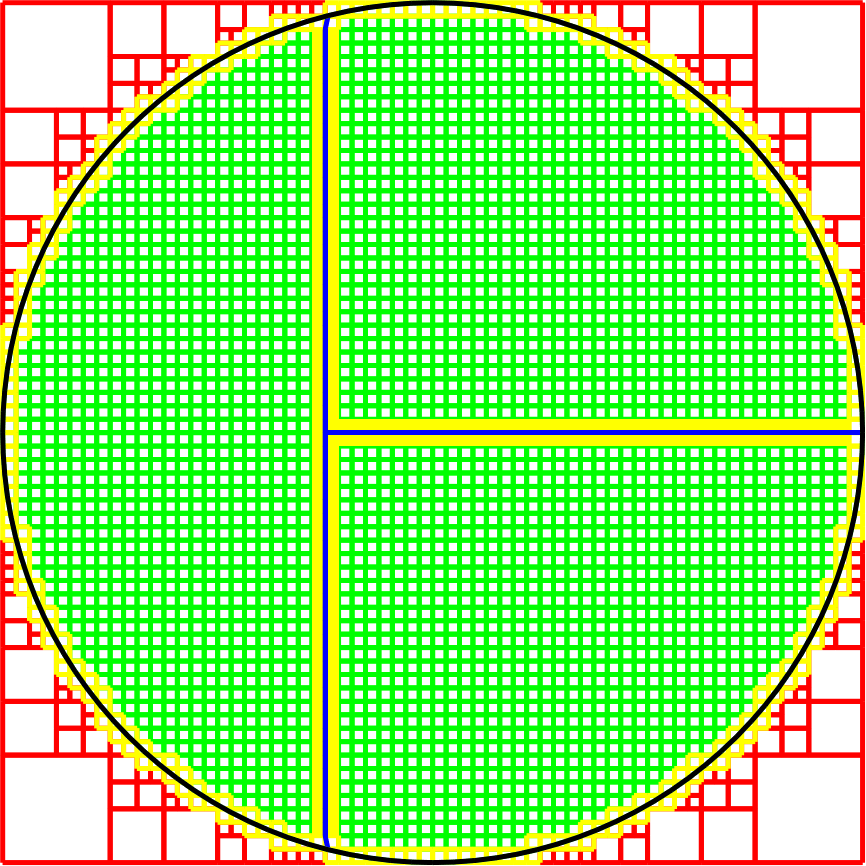
\includegraphics[width=\textwidth]{fig/circulo3_tree.png}}\end{minipage}
	}
	\qquad
	\subfloat[Interfaces do modelo gerada para três subdomínios.]
	{\label{fig:celulas_selecionadas2d_particoes}
		\begin{minipage}[c]{0.45\textwidth}{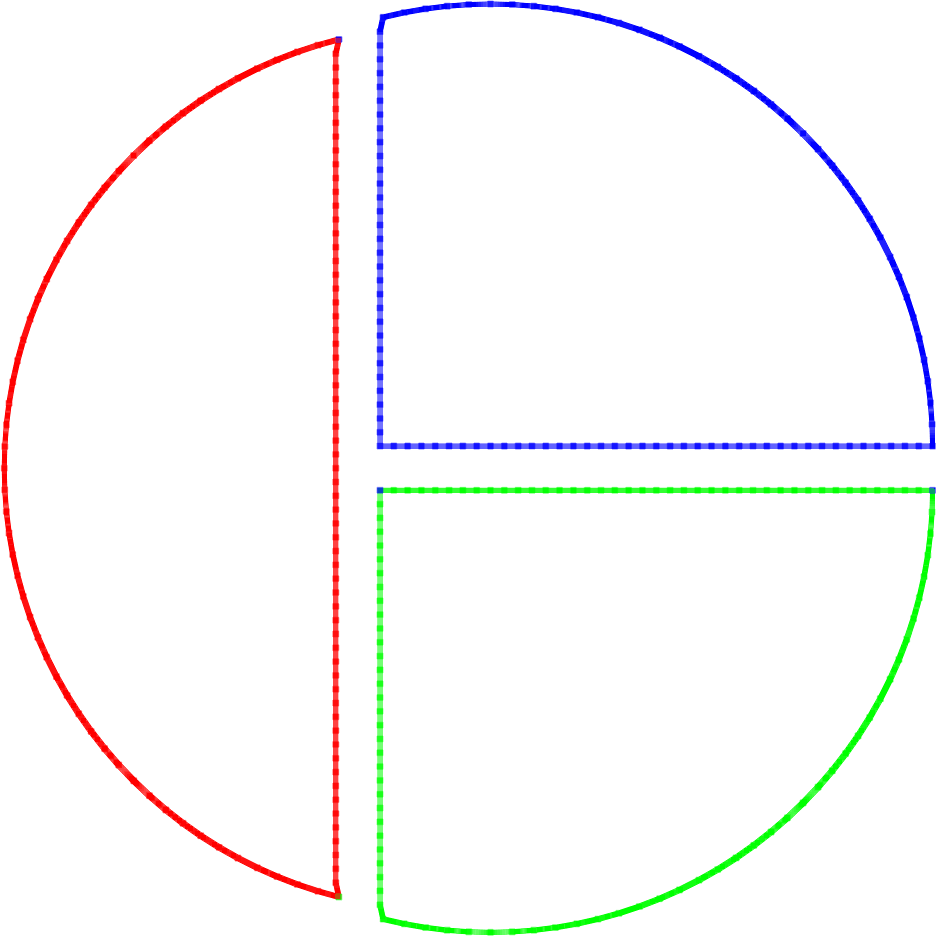
\includegraphics[width=\textwidth]{fig/circulo3.png}}\end{minipage}
	}
	\caption{Células da \textit{quadtree} de estimativa de carga em amarelo escuro serão utilizadas para guiar a criação da borda dos novos subdomínios.}
	\label{fig:celulas_selecionadas2d}
\end{figure}


\begin{figure}[!ht]
	\centering    
	\subfloat[\textit{Octree} de estimativa de carga junto com a BSP de particionamento.]
	{\label{fig:celulas_selecionadas3d_tree}
		\begin{minipage}[c]{0.45\textwidth}{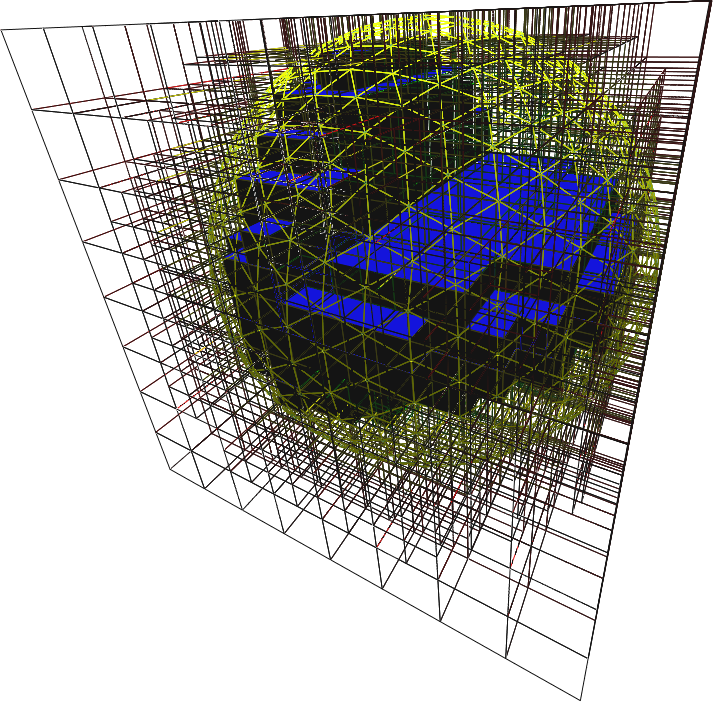
\includegraphics[width=\textwidth]{fig/esfera3_tree.png}}\end{minipage}
	}
	\qquad
	\subfloat[Interfaces do modelo gerada para três subdomínios.]
	{\label{fig:celulas_selecionadas3d_particoes}
		\begin{minipage}[c]{0.45\textwidth}{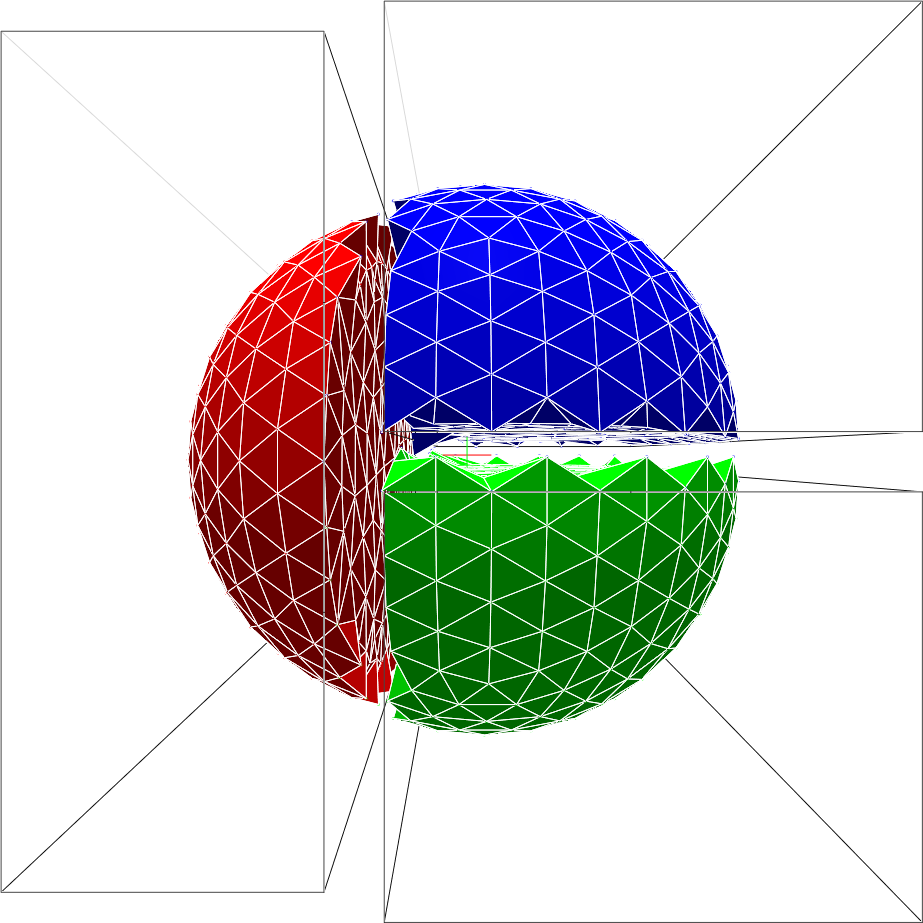
\includegraphics[width=\textwidth]{fig/esfera3.png}}\end{minipage}
	}
	\caption{Células da \textit{octree} de estimativa de carga em azul serão utilizadas para guiar a criação da borda dos novos subdomínios.}
	\label{fig:celulas_selecionadas3d}
\end{figure}


Dentre todas as células da estrutura de estimativa de carga, deve-se selecionar um conjunto de células que fazem interseção com a estrutura de particionamento. As células que não fazem nenhum tipo de interseção com a estrutura de particionamento não estarão nesse conjunto

Células que estão totalmente fora da fronteira do domínio, ou seja, que não estão dentro e nem sobre a fronteira do domínio, mas que também fazem interseção com a estrutura de particionamento, não devem fazer parte desse conjunto. Como essas células estão totalmente fora do domínio, não haverá criação de interfaces nessas regiões; logo, elas devem ser retiradas desse conjunto.

Agora com o conjunto de células internas que interceptam a partição totalmente montado, é realizada a construção da grade de suporte, tendo como base as menores células deste conjunto. Na Figura \ref{fig:criacao_1} as célula em azul escuro são externas ao subdomínio e as azul claro são internas. Após as menores células serem selecionadas o resultado é mostrado na Figura \ref{fig:criacao_2}.


     \begin{figure}[!ht]
     	\centering
     	\subfloat[Exemplo onde a \textit{quadtree} de densidade possui células de tamanhos diferentes.]
     	{\label{fig:criacao_1}
     		\begin{minipage}[c]{0.3\textwidth}{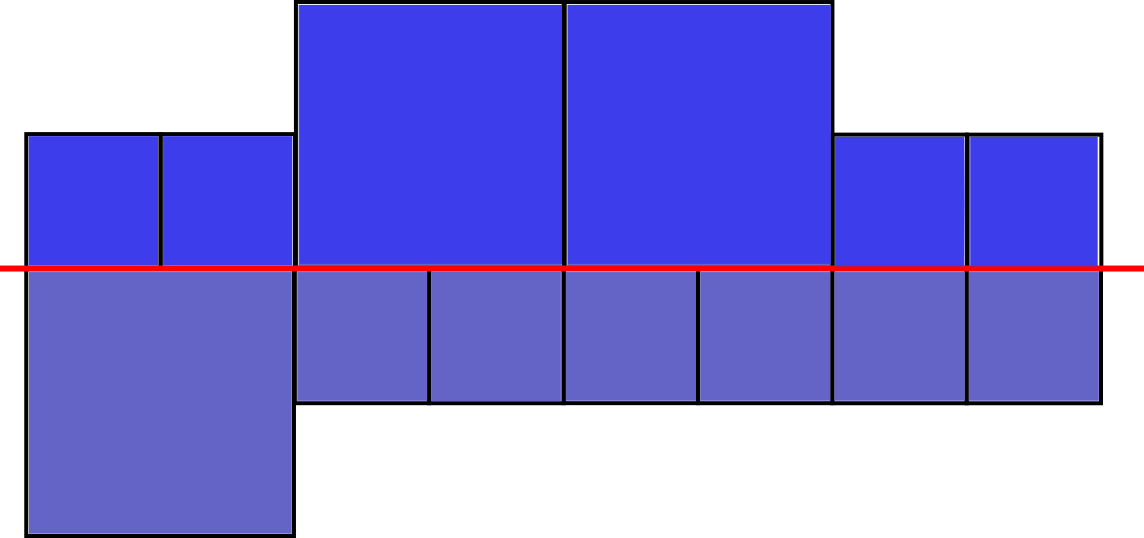
\includegraphics[width=\textwidth]{fig/criacao_1.png}}\end{minipage}
     	}
     	\qquad
     	\subfloat[Células em azul foram as selecionadas para geração da grade de suporte.]
     	{\label{fig:criacao_2}
     		\begin{minipage}[c]{0.3\textwidth}{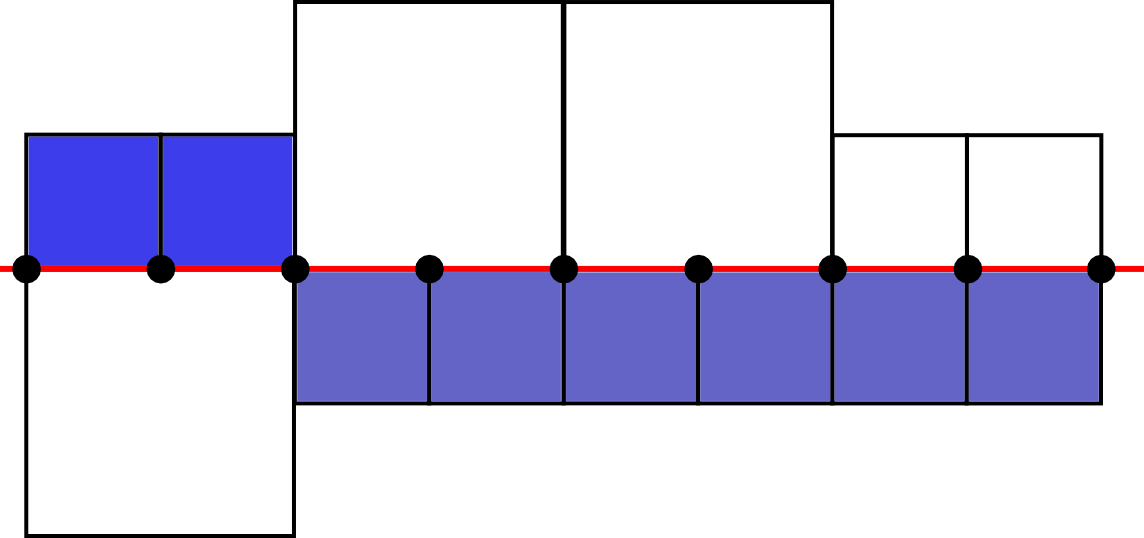
\includegraphics[width=\textwidth]{fig/criacao_2.png}}\end{minipage}
     	}    
     	\caption{Processo de criação da grade de suporte para o caso bidimensional.}
     	\label{fig:criacao_arestas}
     \end{figure}   

No caso bidimensional a grade de suporte é apenas um conjunto de pontos, já no caso tridimensional é feita uma triangulação bidimensional usando padrões nos vértices previamente selecionados. A Figura \ref{fig:grades_modelos} mostra a grade de suporte que foi gerada para um modelo bidimensional e um tridimensional.


     \begin{figure}[!ht]
     	\centering
     	\subfloat[Grade de suporte resultante do corte que passa entre a partição vermelha e a junção da partição azul com a verde da Figura \ref{fig:celulas_selecionadas2d_particoes}.]
     	{\label{fig:grades_modelos2d}
     		\begin{minipage}[c]{0.4\textwidth}{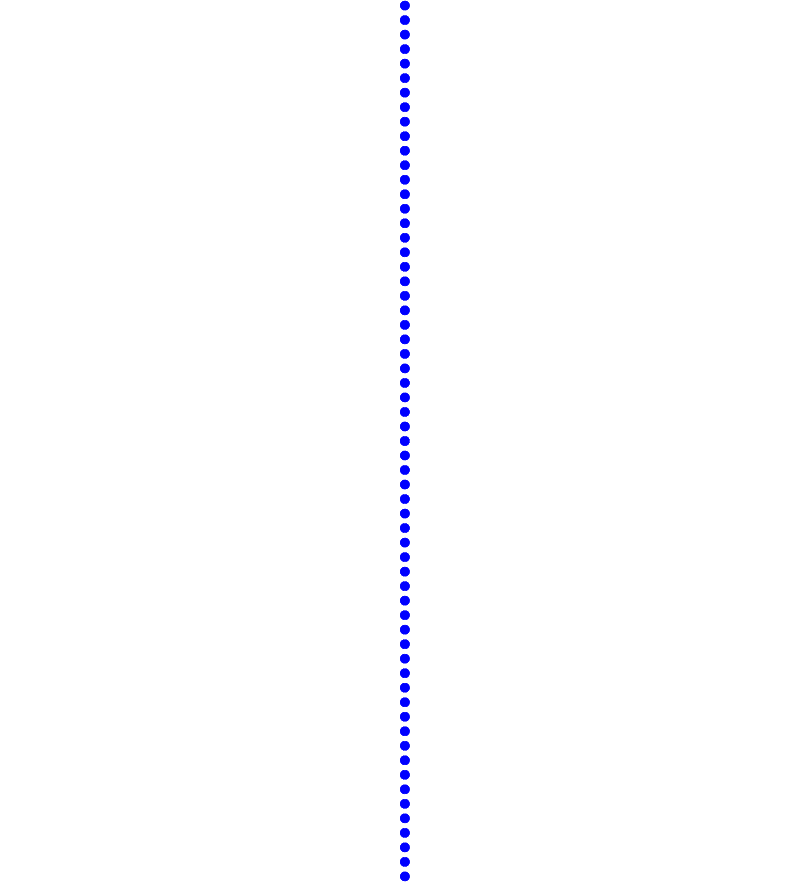
\includegraphics[width=\textwidth]{fig/circulo3_grade.png}}\end{minipage}
     	}
     	\qquad
     	\subfloat[Grade de suporte resultante do corte que passa entre a partição vermelha e a junção da partição azul com a verde da Figura \ref{fig:celulas_selecionadas3d_particoes}.]
     	{\label{fig:grades_modelos3d}
     		\begin{minipage}[c]{0.4\textwidth}{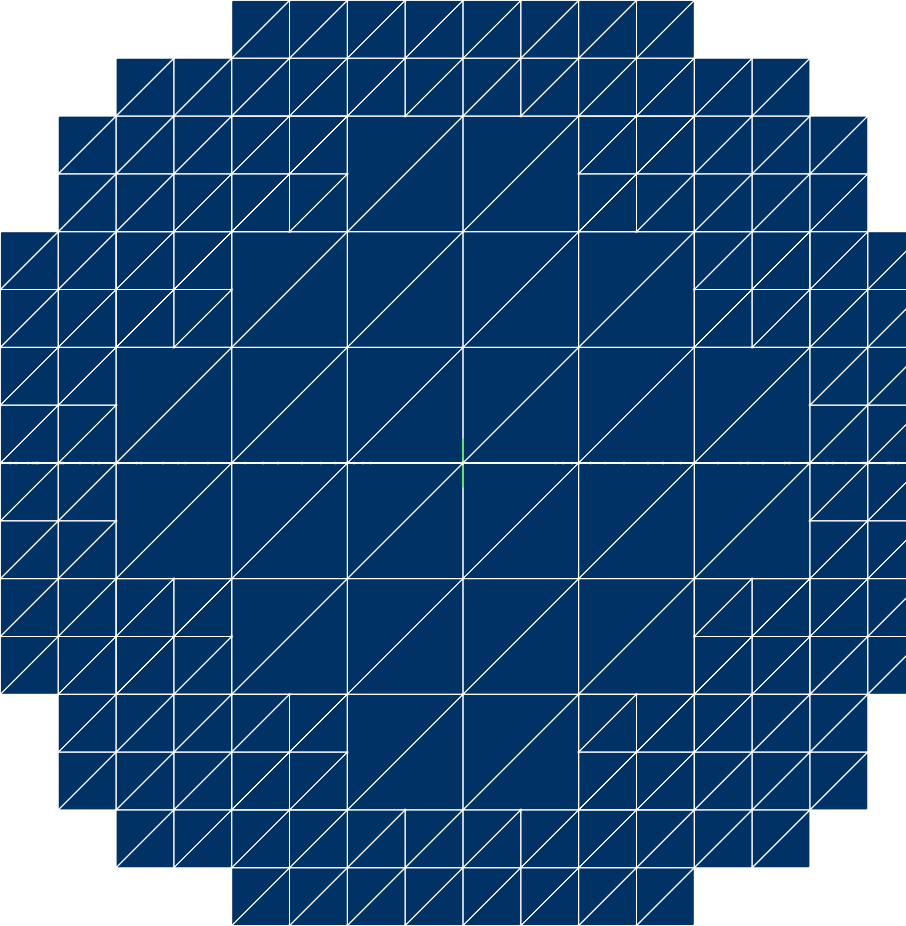
\includegraphics[width=\textwidth]{fig/esfera3_grade.png}}\end{minipage}
     	}    
     	\caption{Grades de suporte para o caso bidimensional e tridimensional.}
     	\label{fig:grades_modelos}
     \end{figure}
     
        
\subsection{Elementos de Interseção}
\label{sec:Elementos_Intersecao}

Algumas partições estarão sobre a fronteira do domínio e alguns de seus elementos terão que se conectar à esta fronteira. O caso bidimensional é simples quando comparado ao caso tridimensional.

No caso bidimensional é feita a interseção das arestas do modelo com o corte posicionado pela BSP de particionamento. O conjunto de arestas resultantes serão as candidatas a fazerem parte da malha de interface. A Figura \ref{fig:circulo_arestas} ilustra o resultado obtido para o caso bidimensional.


\begin{figure}[!ht]
	\centering
	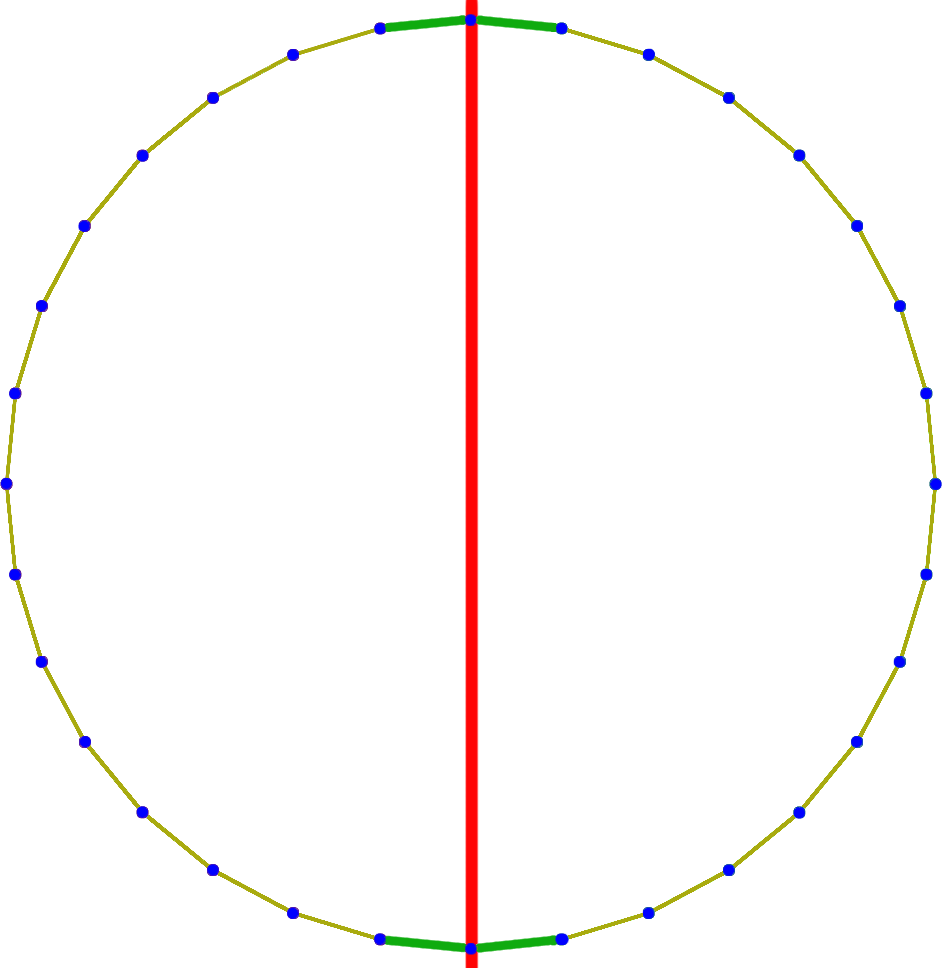
\includegraphics[width=0.35\textwidth]{fig/circulo2_arestas.png}
	\caption{Arestas em verde serão selecionadas ao fazer a interseção do corte feito pela BSP com o modelo.}
	\label{fig:circulo_arestas}
\end{figure}


Já no caso tridimensional a interseção das faces do modelo com o corte posicionado pela BSP de particionamento irá resultar em um conjunto de faces. A Figura \ref{fig:espera_faces} ilustra o resultado obtido para o caso tridimensional. Baseado nestas faces, é necessário encontrar o melhor ciclo de arestas possível.


\begin{figure}[!ht]
   	\centering
   	\subfloat[Interseção do plano de partição da BSP com o modelo. As faces em azul fazem insterseção com o plano.]
   	{\label{fig:espera_modelos_faces}
   		\begin{minipage}[c]{0.4\textwidth}{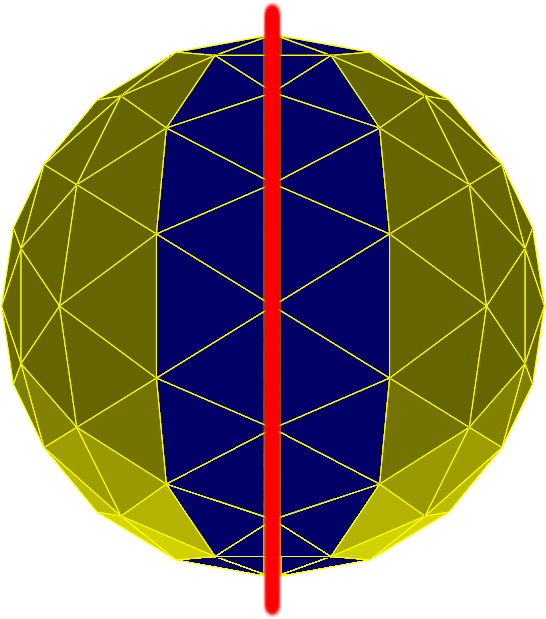
\includegraphics[width=\textwidth]{fig/esfera_simples_particao.png}}\end{minipage}
   	}
   	\qquad
   	\subfloat[Visão lateral das faces que fazem insterseção com o plano de partição da BSP.]
   	{\label{fig:espera_faces_selecionadas}
   		\begin{minipage}[c]{0.4\textwidth}{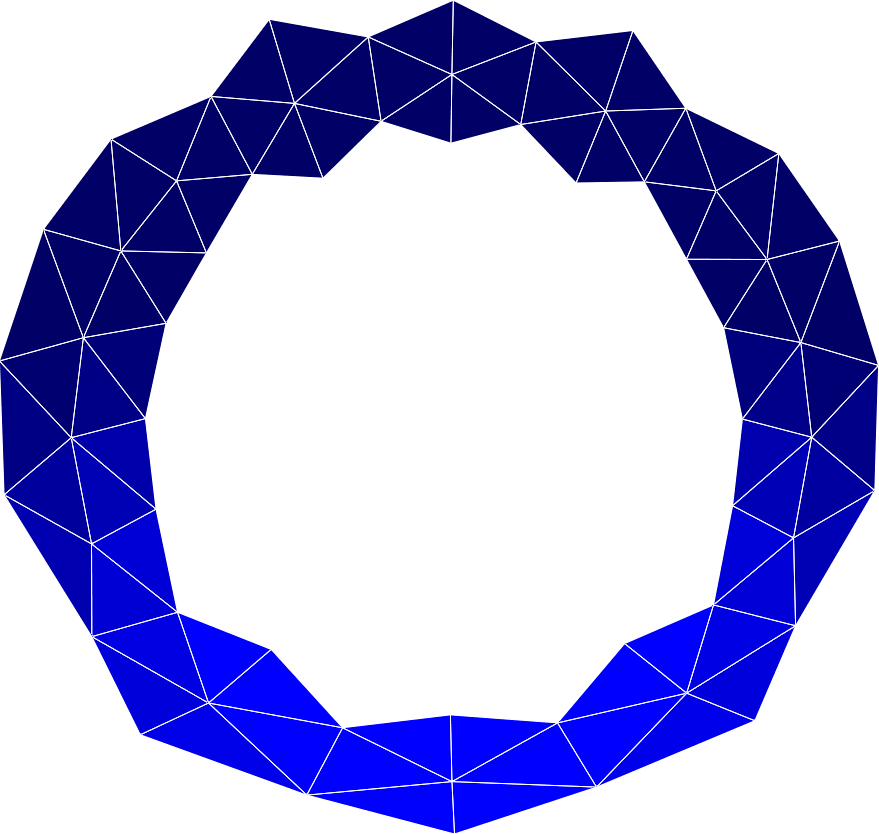
\includegraphics[width=\textwidth]{fig/esfera_simples_anel_faces.png}}\end{minipage}
   	}    
   	\caption{Passos para encontrar o conjunto do faces que fazem interseção com o plano de partição feito pela BSP.}
   	\label{fig:espera_faces}
\end{figure}


O critério de seleção inicial das arestas é obter todas as arestas que interceptam o plano de partição, eliminando aquelas que ficarem soltas ou que formem pequeno ciclos. Ao final é obtido um ciclo, não necessariamente ele será o melhor, por isso é necessário realizar mais um passo de melhoria deste ciclo de arestas. A Figura \ref{fig:melhoria_arestas_ruim1} e \ref{fig:melhoria_arestas_ruim2} ilustram em vermelho o ciclo inicial de arestas encontrado, tendo como base as faces do modelo que interceptaram o plano de partição da BSP.

\begin{figure}[ht]
	\centering
	\subfloat[Modelo 01: Arestas selecionadas inicialmente.]
	{\label{fig:melhoria_arestas_ruim1}
		\begin{minipage}[c]{0.3\textwidth}{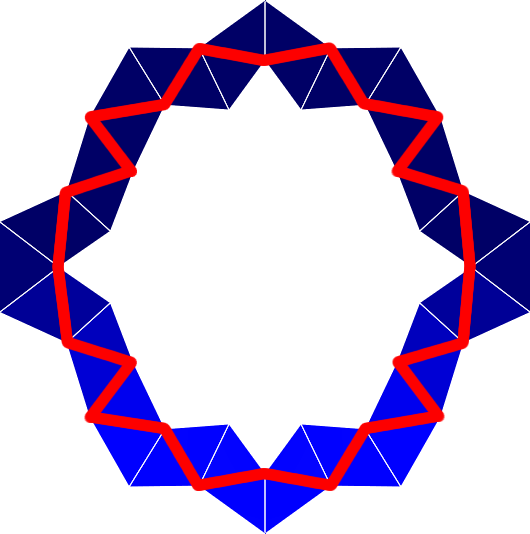
\includegraphics[width=\textwidth]{fig/exemplo_arestas_ruim1.png}}\end{minipage}
	}
	\qquad
	\subfloat[Modelo 01: Melhoria realizada na arestas previamente selecionadas.]
	{\label{fig:melhoria_arestas_bom1}
		\begin{minipage}[c]{0.3\textwidth}{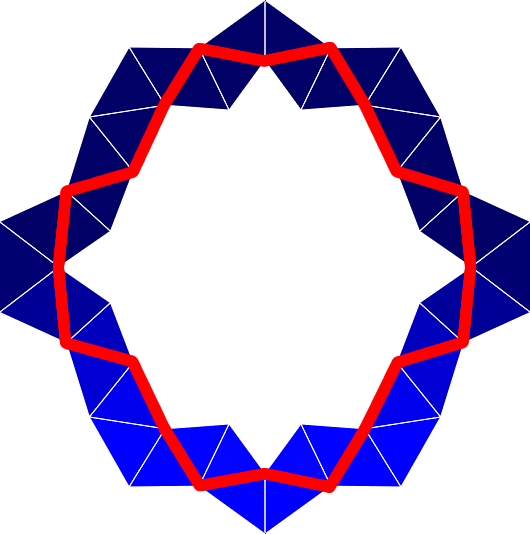
\includegraphics[width=\textwidth]{fig/exemplo_arestas_bom1.png}}\end{minipage}
	}
	
	\subfloat[Modelo 02: Arestas selecionadas inicialmente.]
	{\label{fig:melhoria_arestas_ruim2}
		\begin{minipage}[c]{0.3\textwidth}{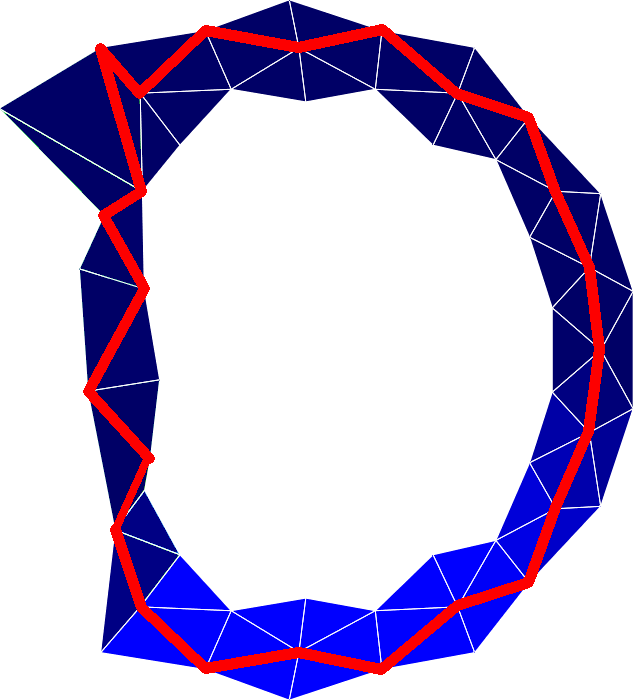
\includegraphics[width=\textwidth]{fig/exemplo_arestas_ruim2.png}}\end{minipage}
	}    
	\qquad
	\subfloat[Modelo 02: Melhoria realizada na arestas previamente selecionadas.]
	{\label{fig:melhoria_arestas_bom2}
		\begin{minipage}[c]{0.3\textwidth}{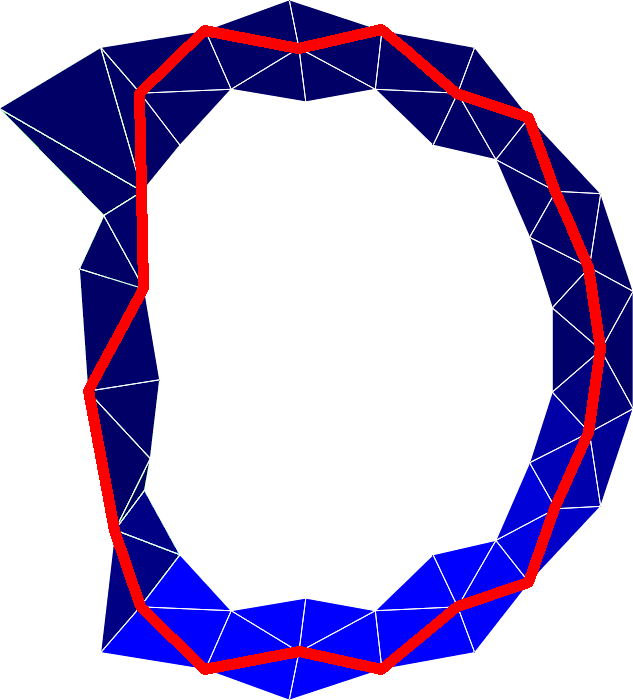
\includegraphics[width=\textwidth]{fig/exemplo_arestas_bom2.png}}\end{minipage}
	}
	\caption{Seleção do ciclo de arestas (em vermelho) com e sem melhoria.}
	\label{fig:melhoria_arestas_apriori}
\end{figure}


A melhoria do ciclo de arestas é feita visando melhorar o ângulo entre as arestas, consequentemente melhorará a malha de interface que será gerada. Para cada par de arestas vizinhas é feita uma verificação se existe uma face que contém estas duas arestas, se existir e o ângulo entre as arestas melhorar, estas duas arestas serão removidas e será adicionada a outra aresta da face encontrada. Um exemplo pode ser visto da Figura \ref{fig:melhoria_arestas_apriori} onde é possível ver as mudanças que ocorreram quando a melhoria foi realizada.

\subsection{Geração da Interface Bidimensional}

No caso bidimensional as arestas da interface são criadas seguindo a grade de pontos encontrada anteriormente. É necessário realizar a junção dessas arestas com o modelo, para isto é feita uma busca nos vértices que fazem interseção com a partição. O vértice que formar o maior ângulo com a interface será o candidato para realizar a junção da interface com o modelo. Ao final desse processo cada partição terá sua fronteira construída e estará pronta para geração da malha, como mostra a Figura \ref{fig:subdominios2D_montados}.


\begin{figure}[!ht]
	\centering
	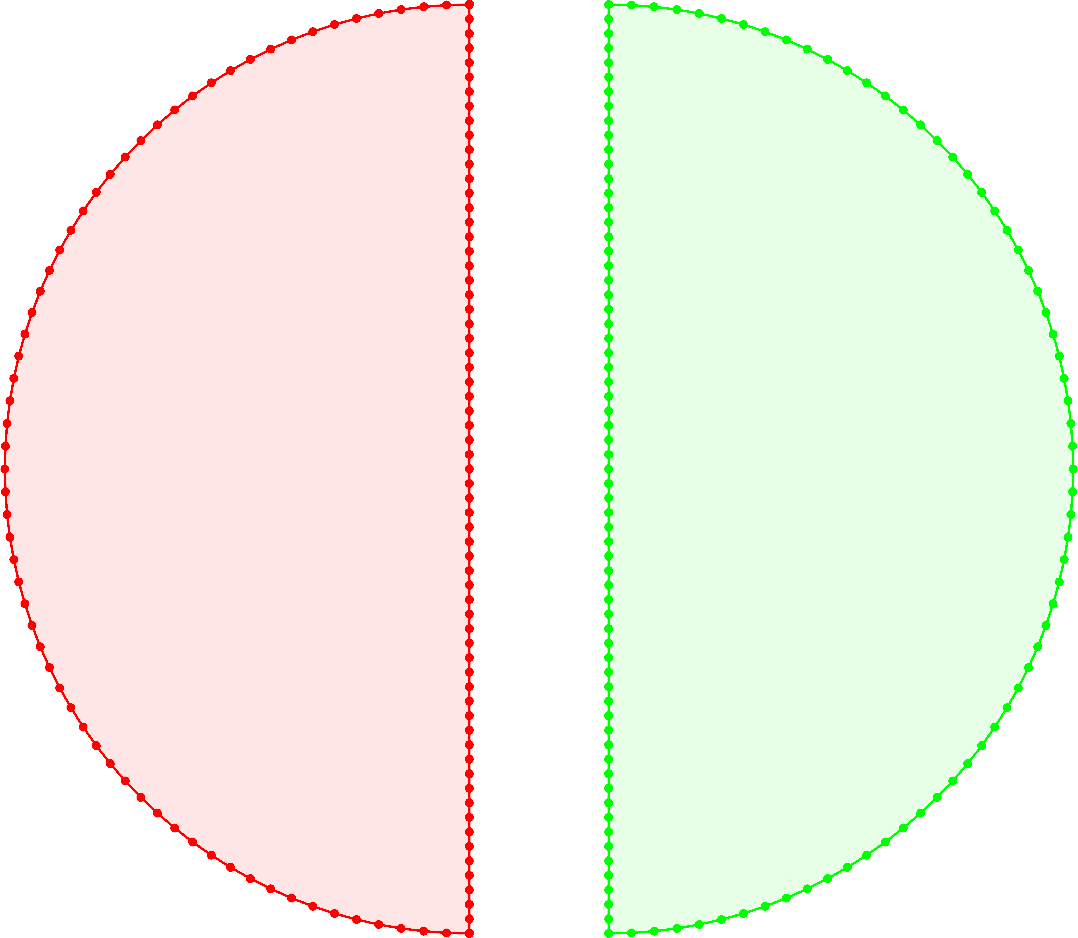
\includegraphics[width=0.3\textwidth]{fig/subdominios2D_montados.png}
	\caption{Subdomínios totalmente criados e prontos para a fase de geração de malha.}
	\label{fig:subdominios2D_montados}
\end{figure}


\subsubsection{Teste de Proximidade}
\label{sec:Teste_proximidade}

Um dos problemas de se utilizar estruturas que geram regiões paralelas aos eixos para particionar domínios é a possibilidade das partições estarem posicionadas em regiões onde os elementos a serem gerados sejam de má qualidade ou até mesmo em posições em que não é possível gerar elementos (a Figura \ref{fig:teste_prox1} mostra um caso da partição estar muito próxima da fronteira). 


\begin{figure}[ht]
	\centering
	\subfloat[Caso em que o tratamento de proximidade é realizado.]
	{\label{fig:teste_prox1}
		\begin{minipage}[c]{0.35\textwidth}{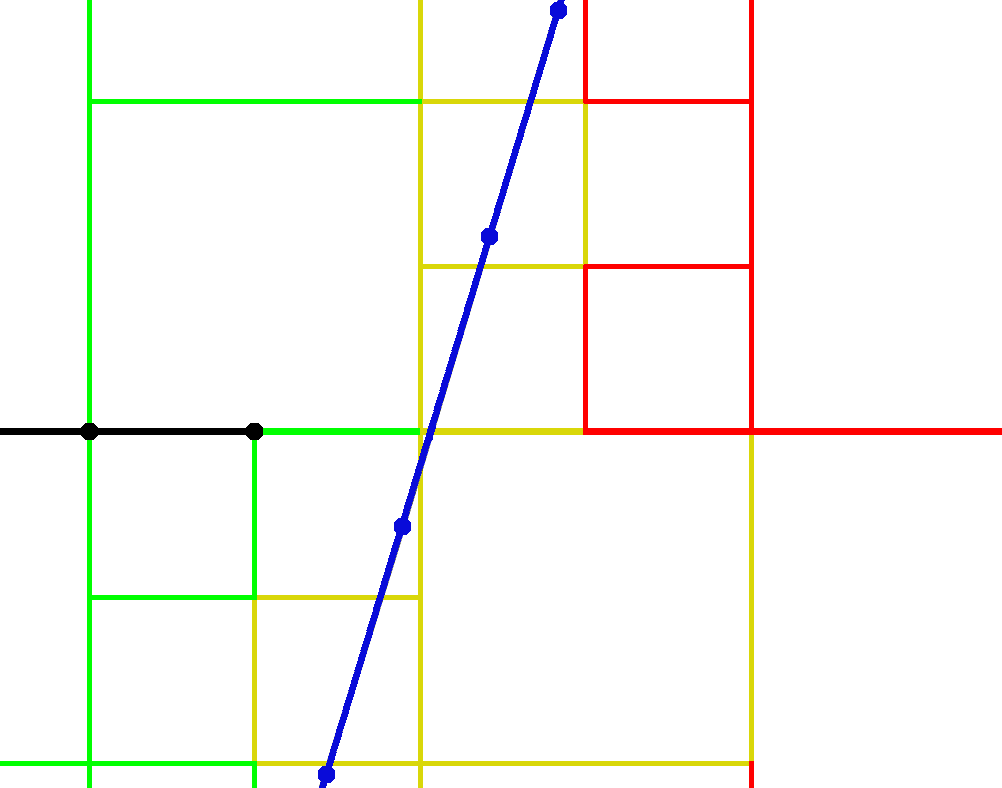
\includegraphics[width=\textwidth]{fig/teste_prox1.png}}\end{minipage}
	}
	\qquad
	\subfloat[Busca pelo vértice da fronteira que forma o maior ângulo entre os candidatos.]
	{\label{fig:teste_prox2}
		\begin{minipage}[c]{0.35\textwidth}{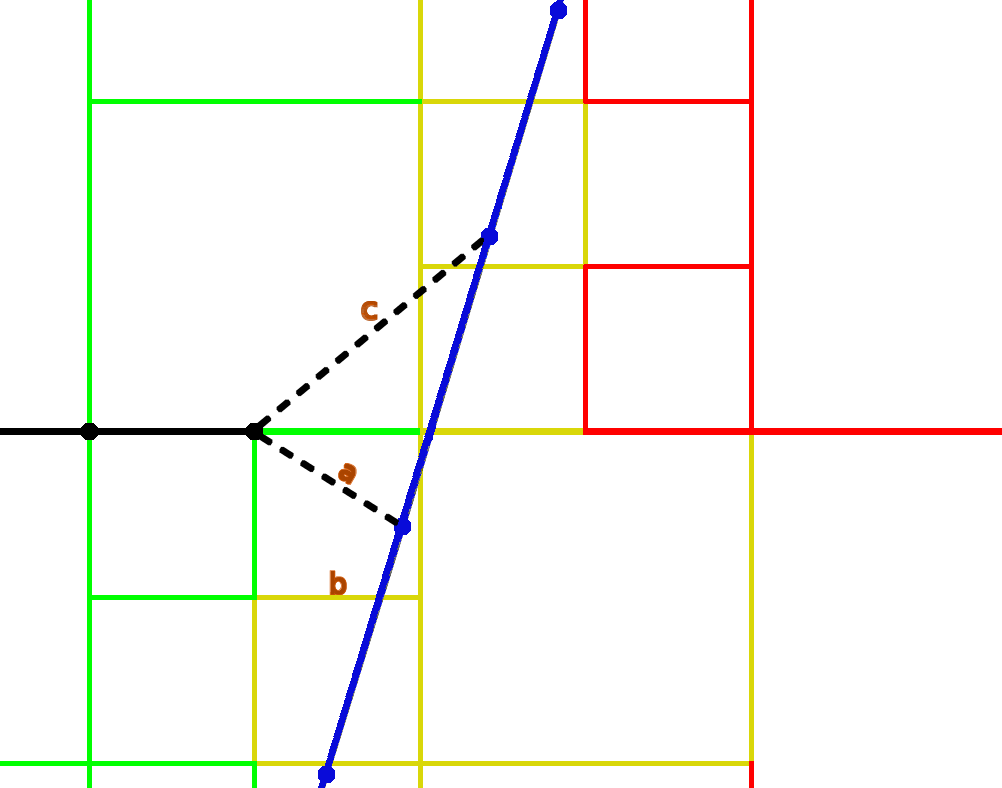
\includegraphics[width=\textwidth]{fig/teste_prox2.png}}\end{minipage}
	}
	
	\subfloat[Aresta criada pelo teste de proximidade.]
	{\label{fig:teste_prox_fim}
		\begin{minipage}[c]{0.35\textwidth}{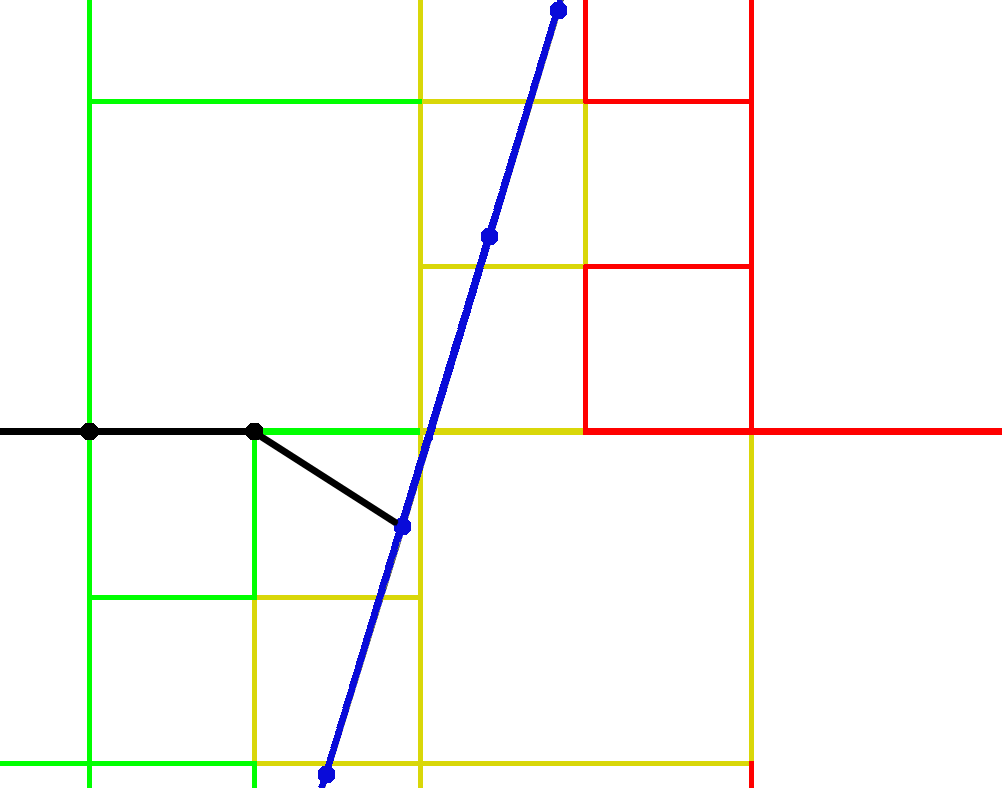
\includegraphics[width=\textwidth]{fig/teste_prox_fim.png}}\end{minipage}
	}    
	\qquad
	\subfloat[Aresta que seria criada caso o teste de proximidade não fosse realizado.]
	{\label{fig:teste_prox_error}
		\begin{minipage}[c]{0.35\textwidth}{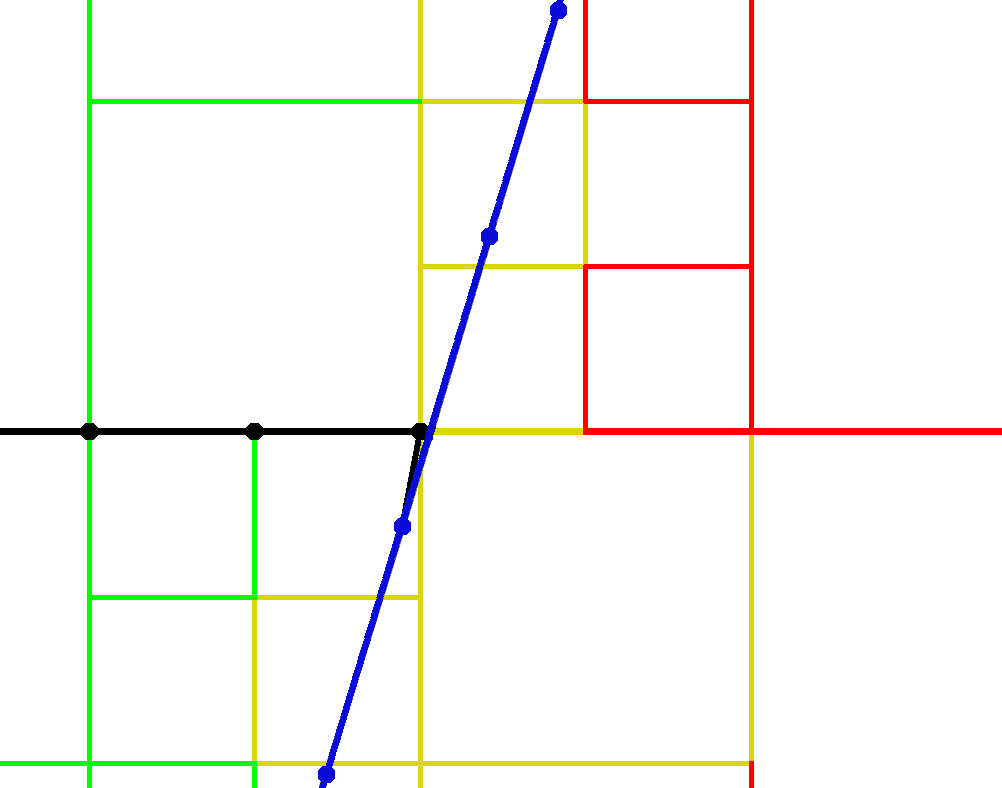
\includegraphics[width=\textwidth]{fig/teste_prox_error.png}}\end{minipage}
	}
	\caption{Possíveis casos no teste de proximidade.}
	\label{fig:teste_prox}
\end{figure}


A busca pelo vértice da fronteira mais próximo que intercepta a partição não garante a qualidade do subdomínio criado, pois, dependendo do refinamento da entrada e do posicionamento do corte da partição, o melhor vértice pode ter uma posição ruim para gerar malha. Se estes casos não forem tratados, o algoritmo de geração da malha possivelmente falhará ou gerará elementos de baixa qualidade.

Para tratar os casos citados, foram implementados testes de proximidade que utilizam as informações das células da estrutura de estimativa de carga. Com esses testes a qualidade da malha melhora além de se evitar possíveis erros na geração da malha.

O teste de proximidade é realizado quando a partição que está sendo criada utiliza uma célula da estrutura de estimativa de carga que intercepta a fronteira de entrada. Se isto ocorrer, será feita uma verificação se a célula da estrutura de estimativa de carga que está sendo testada é classificada como sobre a fronteira do domínio. Em caso afirmativo, será realizada uma busca pelo melhor vértice da fronteira que faz o maior  (Figura \ref{fig:teste_prox2}, onde entre as arestas $a$ e $c$, a melhor será $a$). Se o comprimento desta aresta for menor que o lado $b$ da célula da estrutura estimativa de carga que está sendo utilizada, será gerada a aresta que liga os dois vértices (Figura \ref{fig:teste_prox_fim}). Caso contrário, será criado um novo vértice segundo as informações da grade de suporte.

Esse teste é baseado na ideia de que para um bom elemento ser gerado ele precisa de uma área mínima. Neste trabalho é assumido que esta distância mínima deve ser o tamanho da célula da \textit{quadtree} de estimativa de carga para o caso bidimensional. Com este teste evita-se a criação de arestas com ângulos muito pequenos (Figura \ref{fig:teste_prox_error}) e melhora a qualidade dos elementos que serão gerados.

Esse mesmo teste se aplica a outros casos; um deles é quando a célula da partição tem uma região da sua célula tangente à fronteira de entrada, como mostrado na esquerda da Figura~\ref{fig:teste_prox_passos2}. Neste caso o teste de proximidade será efetuado várias vezes de tal forma que a medida que as arestas vão entrando no teste de proximidade, a região que está muito próxima da borda é transferida para a partição vizinha. Como consequência disso, parte da malha que seria gerada por um processador, será agora tratada pelo vizinho.


\begin{figure}[!ht]
	\centering
	\subfloat[Célula da estrutura de particionamento (em vermelho) juntamente com a borda de entrada.]
	{\label{fig:teste_prox_passos1}
		\begin{minipage}[c]{0.35\textwidth}{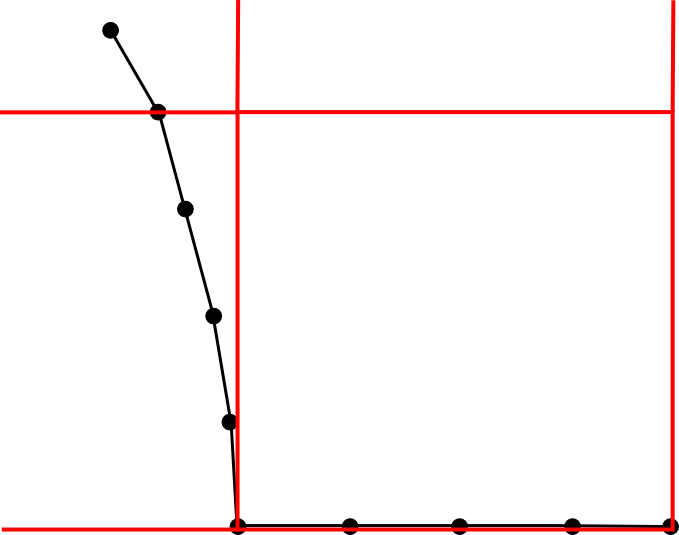
\includegraphics[width=\textwidth]{fig/prox_1.png}}\end{minipage}
	}
	\qquad
	\subfloat[Arestas em azul entram no teste de proximidade.]
	{\label{fig:teste_prox_passos2}
		\begin{minipage}[c]{0.35\textwidth}{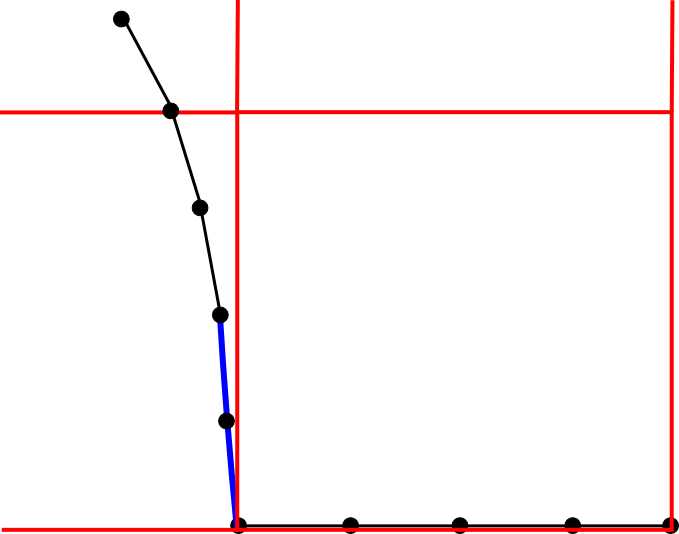
\includegraphics[width=\textwidth]{fig/prox_2.png}}\end{minipage}
	}    
	
	\subfloat[Após o teste de proximidade ser aplicado, o subdomínio azul fica responsável pela região onde as arestas falharam nos testes.]
	{\label{fig:teste_prox_passos3}
		\begin{minipage}[c]{0.35\textwidth}{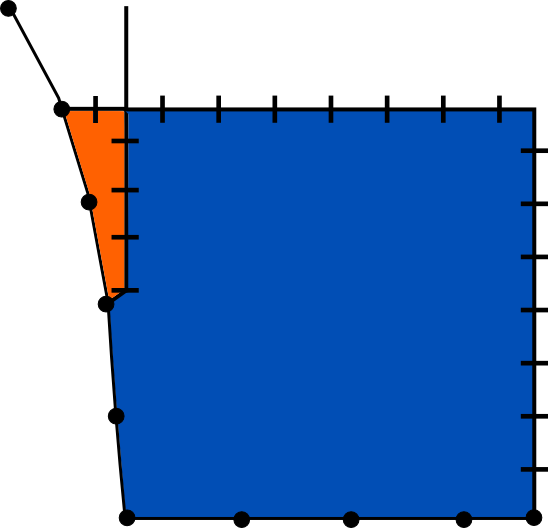
\includegraphics[width=\textwidth]{fig/prox_3.png}}\end{minipage}
	}    
	\qquad
	\subfloat[Subdomínios que seriam gerados sem a realização dos testes de proximidade.]
	{\label{fig:teste_prox_passos4}
		\begin{minipage}[c]{0.35\textwidth}{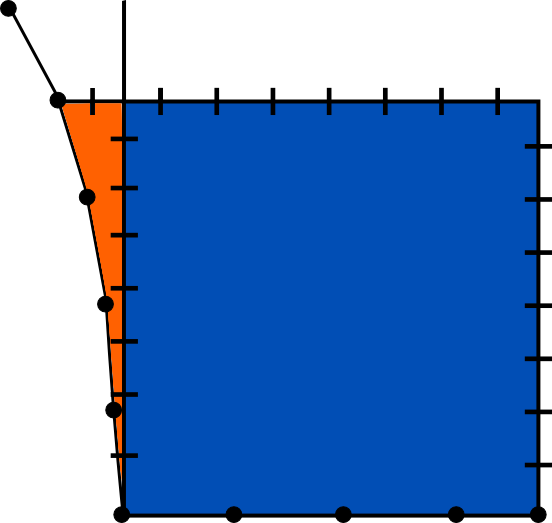
\includegraphics[width=\textwidth]{fig/prox_4.png}}\end{minipage}
	}    
	\caption{Modificações nas regiões realizadas pelo teste de proximidade para evitar elementos ruins.}
	\label{fig:teste_prox_passos}
\end{figure}


\subsubsection{Tratamento de Buracos}
\label{sec:Tratamento_buracos}

Alguns modelos possuem buracos em seus domínios, e, nesses casos, é preciso realizar um teste simples para evitar que sejam criadas arestas que atravessem a fronteira. Esse tratamento é realizado apenas quando uma partição da BSP intercepta algum buraco do modelo.

Quando se tem um buraco que intercepta a partição que está sendo criada, existirão células classificadas como fora da partição entre as que estão classificadas como dentro ou que cruzam a fronteira. O algoritmo tentará gerar uma aresta entre duas células classificadas como internas, mas essa aresta irá cruzar células classificadas como externas ao domínio. 

\begin{figure}[!ht]
	\centering
	\subfloat[Célula da estrutura de particionamento (em vermelho) juntamente com a borda de entrada que contém um buraco.]
	{\label{fig:teste_prox_buraco_passos1}
		\begin{minipage}[c]{0.35\textwidth}{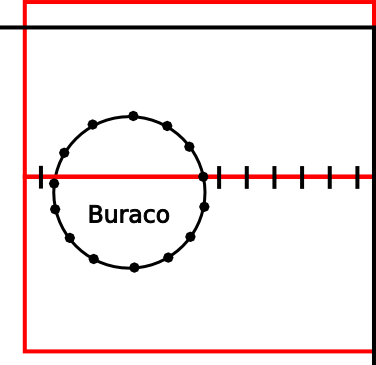
\includegraphics[width=\textwidth]{fig/buraco_1.png}}\end{minipage}
	}
	\qquad
	\subfloat[Detecta-se que uma aresta, que seria criada de $a$ para $b$, passa por um buraco.]
	{\label{fig:teste_prox_buraco_passos2}
		\begin{minipage}[c]{0.35\textwidth}{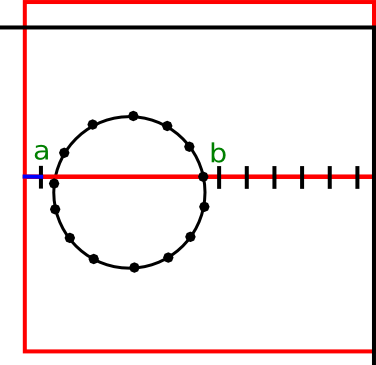
\includegraphics[width=\textwidth]{fig/buraco_2.png}}\end{minipage}
	}    
	\caption{Passos feitos nos tratamentos de buracos.}
	\label{fig:teste_prox_buraco_passos}
\end{figure}

\begin{figure}[!ht]
	\ContinuedFloat
	\centering    
	\subfloat[Teste feito para selecionar a melhor aresta para $a$.]
	{\label{fig:teste_prox_buraco_passos3}
		\begin{minipage}[c]{0.35\textwidth}{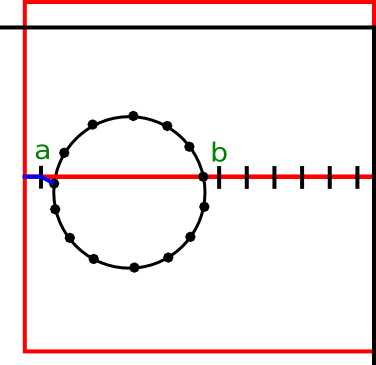
\includegraphics[width=\textwidth]{fig/buraco_3.png}}\end{minipage}
	}    
	\qquad
	\subfloat[Teste feito para selecionar a melhor aresta para $b$.]
	{\label{fig:teste_prox_buraco_passos4}
		\begin{minipage}[c]{0.35\textwidth}{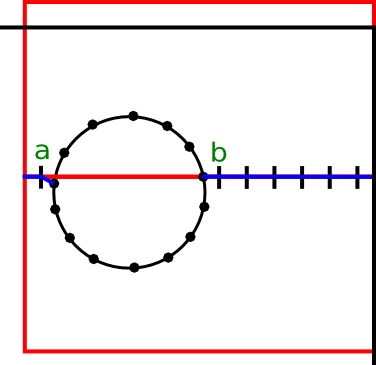
\includegraphics[width=\textwidth]{fig/buraco_4.png}}\end{minipage}
	}    
	\caption{Passos feitos nos tratamentos de buracos (continuação).}
\end{figure}

Quando é detectada uma possível colisão de uma aresta com células externas, serão criadas duas arestas em vez de uma. A primeira conecta o último vértice criado ao vértice mais próximo da primeira interseção do buraco com a partição da BSP (Figura \ref{fig:teste_prox_buraco_passos3}), e a segunda liga o vértice mais próximo da segunda interseção com o buraco a um vértice que será criado de acordo com a grade de suporte (Figura \ref{fig:teste_prox_buraco_passos4}).

\subsection{Geração da Interface Tridimensional}

A interface tridimensional corresponde a uma superfície, sendo a sua fronteira os elementos de interseção mostrado em \ref{sec:Elementos_Intersecao}. A criação desta superfície é feita com a ajuda do algoritmo descrito em \cite{bib:miranda2009surface}. A entrada deste algoritmo é a fronteira da superfície e uma grade de suporte para guiar a criação dos elementos. A grade de suporte utilizada é descrita em \ref{sec:Grade_Suporte}.

Uma translação na grade de suporte deve ser realizada para que o algoritmo de geração da superfície funcione corretamente e para que a malha de interface fique o mais natural possível quando a junção com a superfície for realizada. A translação será feita no mesmo eixo $c$ que o plano de corte da BSP foi posicionado. A grade de suporte deverá ser deslocada para que ela esteja no mesmo plano que o centroide dos vértices do conjunto de elementos de interseção (Equação \ref{eq:traslacao_grade}). 

\begin{equation}
Pos = \frac{\sum_{i=1}^{n} (V_i^c)}{n} \longrightarrow V_i^c = Pos
\label{eq:traslacao_grade}
\end{equation}

Na Equação \ref{eq:traslacao_grade}, a posição do centroide é $Pos$, $n$ é a quantidade de vértices no conjunto de elementos de interseção $V$, $V_i^c$ representa um vértice na iteração $i$ usando a coordenada $c$, que correspondente ao eixo que o corte da BSP de particionamento foi feito. Ao final, a coordenada $c$ de todos os vértices da grade de suporte será $Pos$.

A malha de interface será gerada por avanço de fronteira, tendo como guia a grade de suporte dada como entrada. Esta grade irá auxiliar na criação de elementos, indicando a posição e o tamanho ideal para os novos vértices e elementos. A Figura \ref{fig:geracao_tridimensional} mostra uma visão geral de como o algoritmo de geração da interface funciona.

\begin{figure}[!ht]
	\centering
	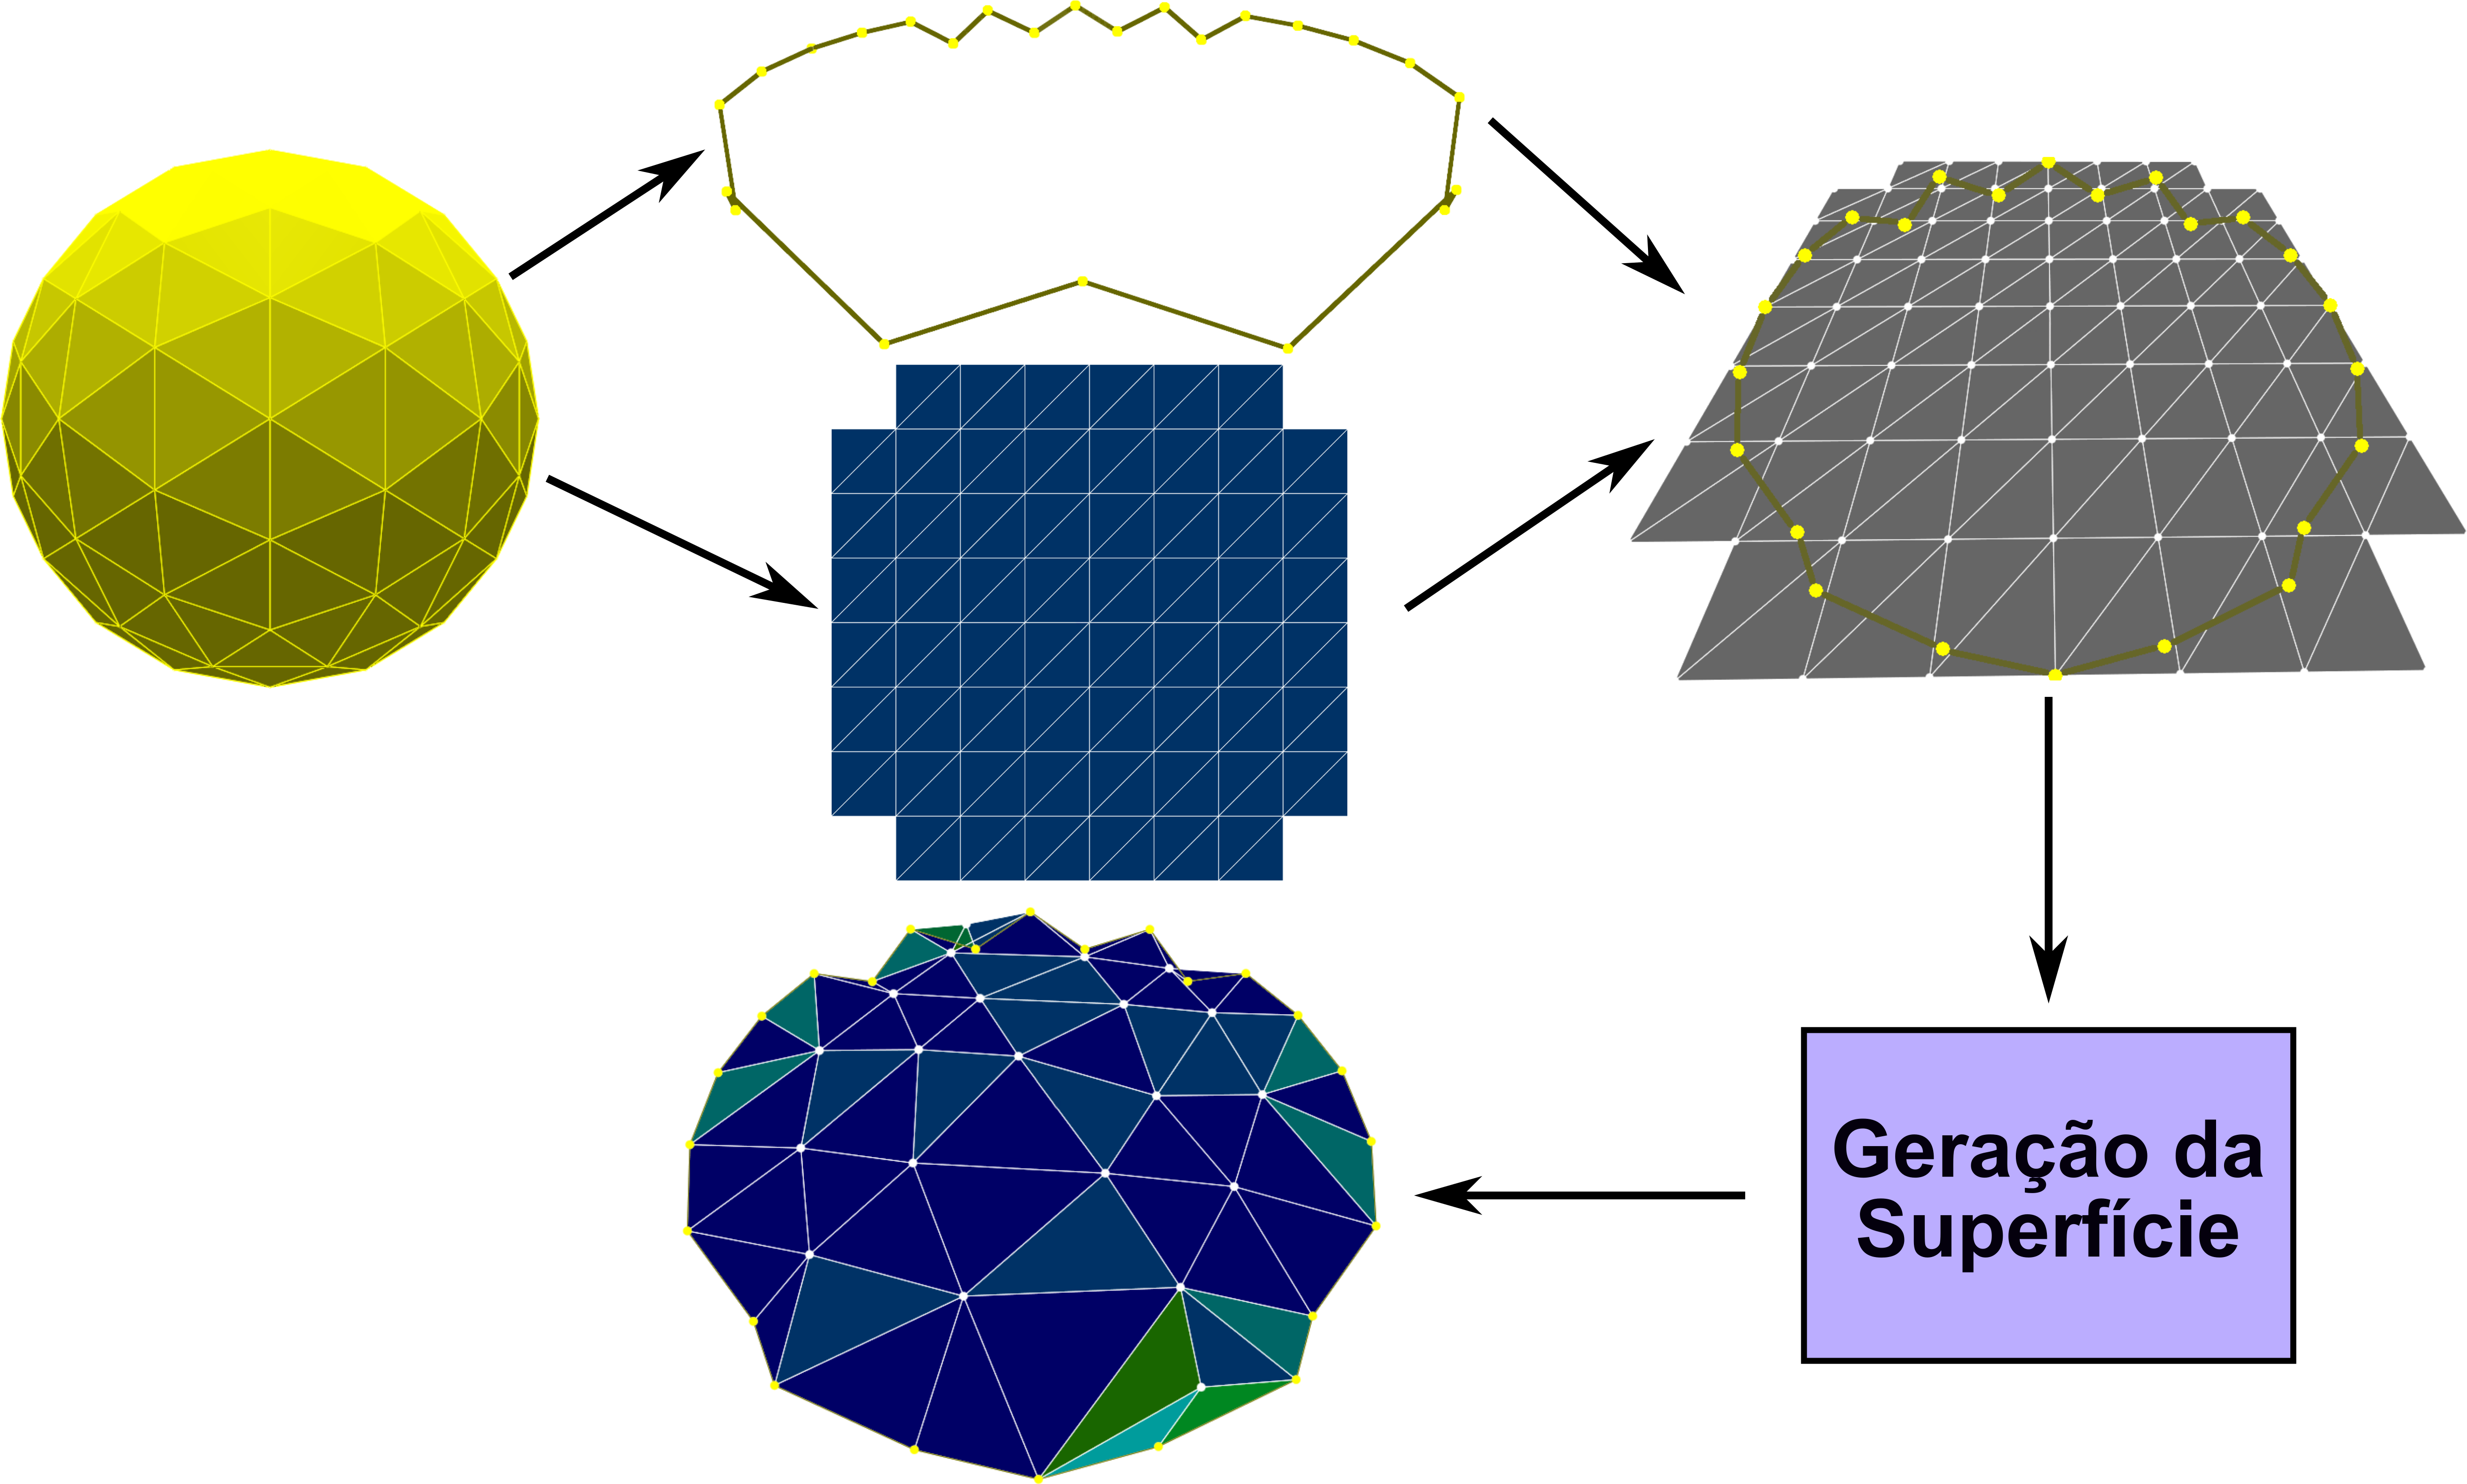
\includegraphics[width=1.0\textwidth]{fig/geracao_tridimensional.png}
	\caption{Etapas para a criação da superfície que será a interface de um subdomínio.}
	\label{fig:geracao_tridimensional}
\end{figure}

Ao final desse processo cada subdomínio estará completamente criado e pronto para a geração da sua malha interna. A Figura \ref{fig:subdominios3D_montados} mostra um modelo particionado em dois subdomínios, é possível notar que as duas partições são complementares, onde a união dos dois subdomínios resulta na mesma superfície de entrada.

\begin{figure}[!ht]
	\centering
	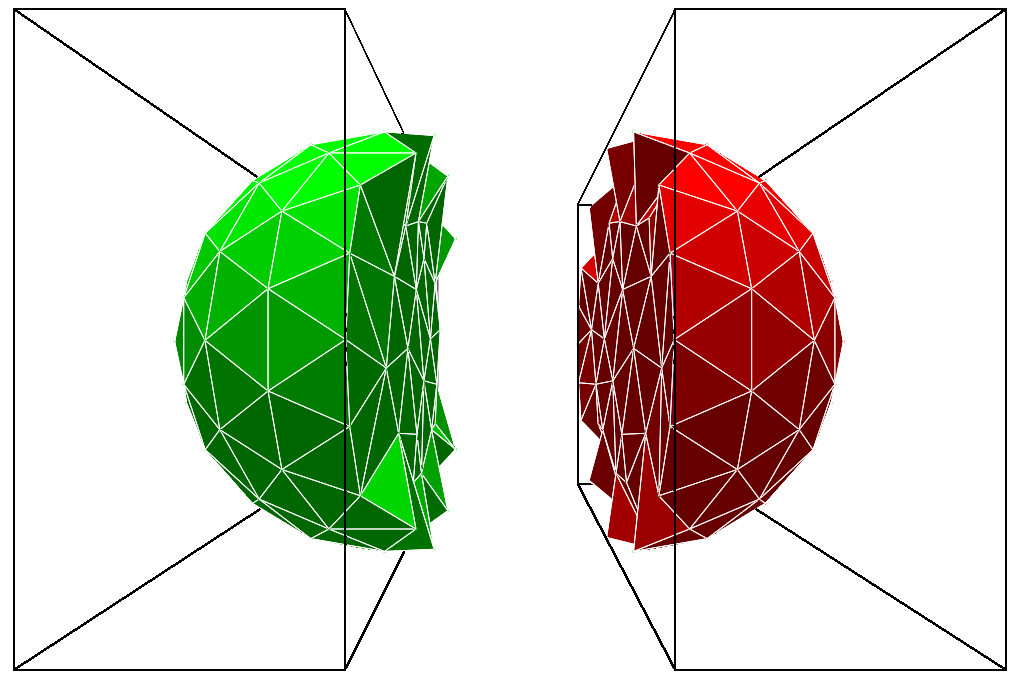
\includegraphics[width=0.5\textwidth]{fig/subdominios3D_montados.png}
	\caption{Subdomínios totalmente criados e prontos para a fase de geração de malha.}
	\label{fig:subdominios3D_montados}
\end{figure}


\section{Balanceamento da Carga}
\label{sec:Balanceamento_de_Carga}


A distribuição das tarefas segue o critério de tentar fazer que todos os processadores gastem praticamente a mesma quantidade de tempo na fase de geração de malha, evitando assim que algum processador fique sobrecarregado ou ocioso.

O número de tarefas gerado é o mesmo de folhas da BSP de particionamento, por isso uma estratégia de balanceamento não-centralizado que utiliza a própria estrutura da BSP para balancear a carga é utilizada neste trabalho.

O balanceamento de carga é realizando aproveitando a estrutura da BSP utilizada para fazer o particionamento do domínio dado como entrada. Inicialmente um único processador é responsável por realizar o primeiro corte, após isso, novos processadores irão sendo ativados para continuar a geração das malhas de interfaces. Ao final do particionamento todos os processadores já estarão com os seus respectivos subdomínios criados e prontos para a geração da malha. A Figura \ref{fig:arvore_balanceamento} mostra a árvore resultante para o balanceamento do modelo da Figura \ref{fig:celulas_selecionadas2d}.


\begin{figure}[!ht]
	\centering
	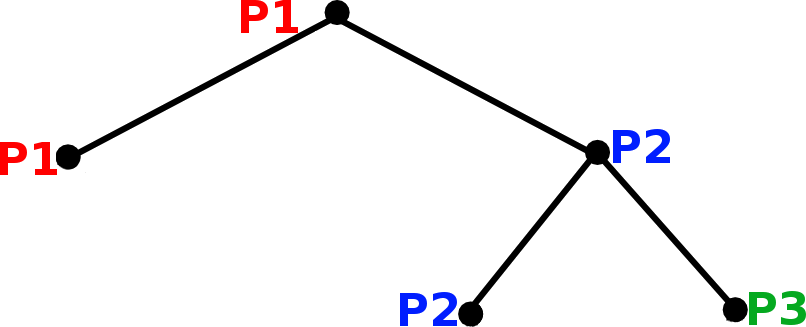
\includegraphics[width=0.5\textwidth]{fig/arvore_balanceamento.png}
	\caption{Balanceamento de carga feito para o modelo da Figura \ref{fig:celulas_selecionadas2d}.}
	\label{fig:arvore_balanceamento}
\end{figure}


Ao chegar nos nós folhas, o processador que tiver responsável por aquela tarefa fará a geração da malha naquele subdomínio. Se a quantidade de tarefas e processadores forem iguais, cada processador receberá uma única tarefa, onde cada tarefa corresponde a uma célula folha da BSP de particionamento. Quando duas células que pertencem a um mesmo nó terminarem de fazer sua computação, um dos processadores dessas células ficará responsável por juntar as duas submalhas e fazer a melhoria na malha resultante. Esse processo é feito para cada par de células que pertence a um mesmo nó da BSP até chegar no nó raiz. A Figura \ref{fig:balanceamento_esfera} ilustra este processo.


\begin{figure}[!ht]
	\centering    
	\subfloat[Processador $P1$ será o responsável por fazer a junção da malha vermelha e azul.]
	{\label{fig:balanceamento_esfera1}
		\begin{minipage}[c]{0.3\textwidth}{\includegraphics[width=\textwidth]{fig/balanceamento1.png}}\end{minipage}
	}
	\qquad
	\subfloat[Processador $P2$ será o responsável por fazer a junção da malha azul e verde.]
	{\label{fig:balanceamento_esfera2}
		\begin{minipage}[c]{0.3\textwidth}{\includegraphics[width=\textwidth]{fig/balanceamento2.png}}\end{minipage}
	}
	\caption{Etapas do balanceamento de tarefas entre os processadores para o moledo da Figura \ref{fig:celulas_selecionadas2d}.}
	\label{fig:balanceamento_esfera}
\end{figure}


\section{Geração da Malha}
\label{sec:Geracao_da_Malha}

Cada processador tem a possibilidade de aplicar algoritmos diferentes se desejado, podendo ser aplicado qualquer técnica de geração de malha que respeite os pré-requisitos citados no início deste capítulo. Foi selecionado uma técnica de Avanço de Fronteira para realizar os testes.

O algoritmo de Avanço de Fronteira utilizado foi desenvolvido em \cite{bib:Miranda99} e \cite{bib:Cavalcante-Neto01}. Foram utilizadas estruturas de dados geométricos para acelerar a busca por vértices candidatos para a geração de um novo triângulo e para a busca de possíveis arestas intersectantes, garantindo uma rápida execução do procedimento de geração de malha.

O processo de geração de malha consiste em três etapas. A primeira é baseada na geometria, tentando gerar elementos de boa qualidade mantendo a validade da malha. A segunda é baseada na topologia, buscando apenas gerar elementos válidos, mesmo eles não sendo de boa qualidade. A última fase é a de geração por retrocesso (\textit{back-tracking}), que tenta finalizar a geração da malha nas áreas onde não foi possível realizar o avanço de fronteira. Vale lembrar que nos casos tridimensionais nem sempre existe uma solução para a geração da malha.

Na versão bidimensional da técnica as duas primeiras fases são suficientes para gerar a malha triangular. Na versão tridimensional nem sempre as duas primeiras fases conseguem finalizar a malha, por isso é necessário o passo de geração por retrocesso (\textit{back-tracking}). A Figura \ref{fig:melhoria_arestas_faces} ilustra o processo de retrocesso aplicado a uma cavidade.


\begin{figure}[ht]
	\centering
	\subfloat[Cavidade em cinza.]
	{\label{fig:melhoria_arestas_faces_ruim1}
		\begin{minipage}[c]{0.25\textwidth}{\includegraphics[width=\textwidth]{fig/backtracking1.png}}\end{minipage}
	}
	\qquad
	\subfloat[Teste de visibilidade sendo feito com o centroide (em azul) e suas arestas de teste.]
	{\label{fig:melhoria_arestas_faces_bom1}
		\begin{minipage}[c]{0.25\textwidth}{\includegraphics[width=\textwidth]{fig/backtracking2.png}}\end{minipage}
	}
	
	\subfloat[Cavidade após remoção de um elemento.]
	{\label{fig:melhoria_arestas_faces_ruim2}
		\begin{minipage}[c]{0.25\textwidth}{\includegraphics[width=\textwidth]{fig/backtracking3.png}}\end{minipage}
	}    
	\qquad
	\subfloat[Malha final, ligada ao centroide, após o retrocesso ser aplicado.]
	{\label{fig:melhoria_arestas_faces_bom2}
		\begin{minipage}[c]{0.25\textwidth}{\includegraphics[width=\textwidth]{fig/backtracking4.png}}\end{minipage}
	}
	\caption{Geração de malhas por retrocesso.}
	\label{fig:melhoria_arestas_faces}
\end{figure}


O processo de geração de malha é complementado com algumas melhorias. Ao todo são três etapas de melhorias, duas delas são modificações na topologia e a outra na geometria. As fases topológicas são a troca de faces (\textit{face swapping}) e a troca de arestas (\textit{edge swapping}), representadas nas Figuras \ref{fig:face_swapping} e \ref{fig:edge_swapping} respectivamente.


\begin{figure}[!ht]
	
	\centering
	\subfloat[Tetraedros adjacentes à face (1, 2, 3).]
	{\label{fig:face_swapping2}
	\begin{minipage}[c]{0.35\textwidth}\centering\includegraphics{fig/markos/face_swapping2.pdf}\end{minipage}}	
	\qquad	
	\subfloat[Tetraedros após a troca de faces ser realizada.]
	{\label{fig:face_swapping3}
	\begin{minipage}[c]{0.35\textwidth}\centering\includegraphics{fig/markos/face_swapping3.pdf}\end{minipage}}
	
	\caption{Troca de faces.}
	
	\label{fig:face_swapping}
	
\end{figure}


\begin{figure}[!ht]
	
	\centering
	\subfloat[Tetraedros adjacentes à aresta (1, 2).]
	{\label{fig:edge_swapping2}
	\begin{minipage}[c]{0.35\textwidth}\centering\includegraphics[scale=1.3]{fig/markos/edge_swapping3.pdf}\end{minipage}}
	\qquad	
	\subfloat[Tetraedros após a troca.]
	{\label{fig:edge_swapping3}
	\begin{minipage}[c]{0.35\textwidth}\centering\includegraphics[scale=1.3]{fig/markos/edge_swapping4.pdf}\end{minipage}}	
	\caption{Troca de arestas, com três tetraedros adjacentes (caso inverso à troca de faces).}	
	\label{fig:edge_swapping}
	
\end{figure}


Na fase geométrica é aplicada uma suavização de Laplace, onde os vértices internos da malha são movidos caso os elementos suavizados sejam melhores que o pior elemento antes da suavização. Esta suavização consiste em mover um vértice interno da malha de tal forma que ele se aproxime do centroide do polígono definido pelos seus vértices adjacentes, seguindo a Equação \ref{eq:laplace}. 


\begin{equation}
X_V^{n+1} = X_V^{n} + \phi \frac{\sum_{i=1}^m (X_i^n - X_V^n)}{m}
\label{eq:laplace}
\end{equation}

\noindent
onde, $X_V^{n}$ é a posição do vértice $V$ na iteração de suavização $n$, $m$ é o número de vértices adjacentes a $V$ por algum tetraedro. $i$ corresponde o i-ésimo vértice adjacente a $V$, $X_V^{n}$ é a posição do i-ésimo vértice adjacente a V na iteração de suavização $n$, e $\phi$ é o parâmetro de relaxamento, normalmente ajustado para um valor entre 0 e 1 (neste trabalho, o valor de $1$ foi utilizado para $\phi$). A Figura \ref{fig:laplace} ilustra como a suavização é feita para $\phi=1,0$.



\begin{figure}[!ht]
	\centering
	\subfloat[Polígono formado pelos vértices adjacentes a $V$ (em vermelho).]
	{\label{fig:laplace1}
		\begin{minipage}[c]{0.25\textwidth}{\includegraphics[width=\textwidth]{fig/laplace1.png}}\end{minipage}
	}
	\qquad
	\subfloat[Centroide do polígono em azul.]
	{\label{fig:laplace2}
		\begin{minipage}[c]{0.25\textwidth}{\includegraphics[width=\textwidth]{fig/laplace2.png}}\end{minipage}
	}
	\qquad	
	\subfloat[Resultado final da suavização de Laplace.]
	{\label{fig:laplace3}
		\begin{minipage}[c]{0.25\textwidth}{\includegraphics[width=\textwidth]{fig/laplace3.png}}\end{minipage}
	}    
	\caption{Suavização de Laplace feita para $\phi=1,0$.}
	\label{fig:laplace}
\end{figure}


\section{Junção e Finalização da Malha}

A junção da malha é realizada seguindo a estrutura da BSP de particionamento de baixo para cima. Cada nó da árvore da BSP corresponde a um processador. A junção das malhas é realizada sempre que dois nós irmãos acabam a fase de geração de malha, um dos processadores ficará responsável pelo processamento e o outro será liberado. A alocação das tarefas foi previamente feita conforme explicado na Seção \ref{sec:Balanceamento_de_Carga}. A Figura \ref{fig:arvore_juncao} mostra a árvore BSP para 8 partições, cada partição é atribuída a um processador.

\begin{figure}[!ht]
	\centering
	\includegraphics[width=0.5\textwidth]{fig/arvore.png}
	\caption{Árvore da BSP de particionamento usada na junção das partições. Em cada nó é mostrado o processador responsável pela geração da malha ou da sua junção/melhoria.}
	\label{fig:arvore_juncao}
\end{figure}


A finalização da malha é realizada logo após a junção dos subdomínios e consiste em melhorias como as descritas na Seção \ref{sec:Geracao_da_Malha}. As melhorias são aplicadas nas interfaces dos subdomínios juntamente com certas camadas de elementos adjacentes a elas. A Figura \ref{fig:finaliza} mostra um mesmo modelo bidimensional com e sem as melhorias nas interfaces.

\begin{figure}[!ht]
	\centering
	\subfloat[Junção das malhas geradas nos diversos processadores.]
	{\label{fig:finaliza1}
		\begin{minipage}[c]{0.35\textwidth}{\includegraphics[width=\textwidth]{fig/finaliza1.png}}\end{minipage}
	}
	\qquad
	\subfloat[Malha resultante depois do último refinamento.]
	{\label{fig:finaliza2}
		\begin{minipage}[c]{0.35\textwidth}{\includegraphics[width=\textwidth]{fig/finaliza2.png}}\end{minipage}
	}
	\caption{Finalização da malha: junção das malhas geradas pelos processadores (à esquerda) e malha refinada final (à direita).}
	\label{fig:finaliza}
\end{figure}

A melhoria da malha é feita na região onde a malha de interface foi construída, juntamente com algumas camadas de elementos adjacentes. Essas camadas são os elementos adjacentes à malhas de interface. Foi verificado em \cite{bib:Ito07} que duas camadas de elementos são suficientes para se obter uma boa malha ao final. A camada $0$ consiste dos próprios segmentos da fronteira, e a camada $N$ compreende os elementos presentes na camada $N-1$ mais seus elementos adjacentes. Depois dessa etapa, a malha está completamente gerada em todo o modelo.


\section{Considerações Finais}

Este capítulo apresentou uma técnica \textit{a priori} para particionamento de malhas para geração em paralelo de malhas. Todos os passos necessários para o entendimento da técnica foram descritos e ilustrados. Este trabalho foi desenvolvido para aceitar entradas bidimensionais ou tridimensionais, podendo-se ainda utilizar qualquer algoritmo para a geração da malha em paralelo.

A grande vantagem deste trabalho é a excelente estimativa de carga feita por uma estrutura de dados espacial; um particionamento nos eixos que busca um corte no modelo que melhor divide a carga entre as partes geradas; e o modelo de criação das interfaces \textit{a priori} que gera subdomínios totalmente independentes, possibilitando assim a utilização de diferentes técnicas de geração de malha com uma baixa comunicação entre as tarefas.			% Tema principal
\chapter{Trabalhos Relacionados}\label{cap3}


Em Computação de Alto Desempenho é conhecido que, para um bom algoritmo paralelo executar, é preciso uma boa estratégia para a divisão da entrada e para a junção das várias soluções ao final. 

Há ainda a preocupação com a distribuição das tarefas entre os processadores, levando em conta que, ao final, todos eles devam ter realizado uma quantidade similar de processamento, evitando que alguns processadores fiquem ociosos enquanto outros estão sobrecarregados. Se isto acontecer, significa que a carga foi devidamente balanceada entre os processadores.

A geometria computacional é a área da computação que estuda soluções e estruturas de dados para problemas geométricos. O seu enfoque é buscar soluções sob o ponto de vista da análise de complexidade de algoritmos. Entre os problemas estudados estão a construção de fechos convexos, triangulações, ordenação de pontos espaciais, interseções de retas/planos, malhas e outros mais.

Neste capítulo, é apresentado inicialmente alguns conceitos necessários para um melhor entendimento dos trabalhos que estão sendo desenvolvidos nos últimos anos na área de particionamento de domínios para geração em paralelo de malha. Logo em seguida será apresentado os trabalhos relacionados a particionamento de domínios, dando ênfase no modo que é tratada a subdivisão dos domínios e a estimativa de carga em cada técnica apresentada. 


\section{Conceitos e Definições}\label{Geometria computacional}

\subsection{Geometria Computacional}\label{Geometria computacional}

A geometria computacional é a área da computação que estuda soluções e estruturas de dados para problemas geométricos. O seu enfoque é buscar soluções sob o ponto de vista da análise de complexidade de algoritmos. Entre os problemas estudados estão a construção de fechos convexos, triangulações, ordenação de pontos espaciais, interseções de retas/planos, malhas e outros mais.

\subsubsection{Fecho Convexo}

O fecho convexo de um conjunto finito de pontos é o menor conjunto convexo que contém tais pontos. Segundo \cite{bib:Carvalho91} um conjunto $K$ do $\Re^{n}$, sendo $n$ um inteiro não negativo, é convexo se quaisquer que sejam  $x \in K$, $y \in K$ e $0 \leq \lambda \leq 1$, $\lambda \in \Re$ , tem-se $\lambda x + (1-\lambda)y \in K $. Ou seja, todas as combinações convexas dos elementos de $K$ pertencem a $K$. Um ponto $p$ é dito ser combinação convexa dos pontos $p_{i} \in K$  se $p = \displaystyle\sum_{i=1}^{|K|} p_{i}\lambda_i $, sendo $ \displaystyle\sum_{i=1}^{|K|} \lambda_i = 1 $.

Um ponto $w \in K$ é um ponto extremo de $K$ se não pode ser conectado a um elemento de $K$ por um segmento de reta aberto pertencente a $K$. O fecho convexo de um conjunto finito $C$ de pontos no $\Re^{n}$, sendo $n$ um inteiro não negativo, é o conjunto de todas as combinações convexas de elementos de $C$. Em outras palavras pode-se dizer que o fecho convexo é um conjunto finito de pontos com menor área geométrica que engloba todos os pontos do conjunto (Figura \ref{fig:fecho convexo}).

 \begin{figure}[htbp]
     \centering
     \includegraphics[width=0.5\textwidth]{fig/fecho_convexo.png}
     \caption{Conjunto de pontos e o seu fecho convexo.} 
     \label{fig:fecho convexo}
 \end{figure}

\subsubsection{Ponto de Steiner}

No triângulo ABC, sejam:
\begin{itemize}
  \item A’ o simétrico de A em relação a G
  \item B’ o simétrico de B em relação a G
  \item C’ o simétrico de C em relação a G;
\end{itemize}

As três circunferências definidas pelos conjuntos de ternos de pontos AB’C’, BA’C’, CA’B’ intersectam-se num ponto do circuncírculo - ponto de Steiner. A cada uma das três circunferências dá-se o nome de “círculo de Steiner”, como mostra a figura \ref{fig:steiner}.

 \begin{figure}[htbp]
     \centering
     \includegraphics[width=0.8\textwidth]{fig/steiner.png}
     \caption{Ponto de Steiner para um triângulo ABC.} 
     \label{fig:steiner}
 \end{figure}

\subsubsection{Triangulação e Malha}

Triangulações são muitas vezes chamadas de malhas ou usadas como malhas, como no caso do método dos elementos finitos (MEF), já que malha é uma união de elementos, que podem ser triângulos, por exemplo. Pode-se definir uma malha $M$ de uma maneira genérica como:

\begin{itemize}
 \item $\varOmega = \bigcup\limits_{k \in M} k $, onde $\varOmega$ é um domínio finito limitado,
 \item O interior de cada elemento $k$ em $M$ é não vazio,
 \item A interseção do interior de dois elementos de $M$ é vazia.
\end{itemize}

Uma triangulação também é uma malha, mas nem toda malha é uma triangulação. Neste trabalho quando for mencionado malha, será sempre a malha que respeita as mesmas propriedades de uma triangulação. A definição de triangulação segundo \cite{bib:Triangulations_applications} diz que:

\begin{itemize}
  \item Nenhum triângulo pertencente à triangulação pode ter pontos colineares.
  \item A interseção do interior de quaisquer dois triângulos pertencentes à triangulação é vazia.
  \item As bordas de 2 triângulos quaisquer só podem fazer interseção com vértices ou arestas.
  \item A união de todos os triângulos da triangulação é igual ao domínio.  
  \item O domínio deve ser conectado.
  \item Não deve existir buracos na triangulação, a menos que eles sejam definidos como entrada.
  \item Se um triângulo está na borda da triangulação então ele faz interseção por aresta no máximo dois triângulos.
\end{itemize}


Existem malhas de diferentes geometrias e dimensões. Caso a topologia de elementos e vértices da malha siga alguma regra simples de indexação, essa malha será definida como estruturada, caso contrário, ela é definida como não-estruturada. Nas malhas estruturadas o conhecimento dos vizinhos de cada elemento não depende do armazenamento ou existência desta informação. Já nas não-estruturadas, para se ter conhecimento dos vizinhos, é necessário armazenar ou calcular estas informações. Existem ainda as malhas mistas, que combinam malhas estruturadas e não-estruturadas (Figura \ref{fig:est_e_n_est}).

As malhas também podem ser classificadas de acordo com a geometria dos seus elementos, já que não são necessariamente formadas somente de triângulos.. Para malhas bidimensionais, por exemplo, elas podem ser de elementos triangulares ou quadrilaterais, por exemplo, como mostra a Figura \ref{fig:est_e_n_est}.

 \begin{figure}[htbp]
     \centering
     \includegraphics[width=0.5\textwidth]{fig/est_e_n_est.png}
     \caption{Exemplo de malha quadrilateral estruturada e não-estruturada triangular.} 
     \label{fig:est_e_n_est}
 \end{figure}
 
Para muitas aplicações, a qualidade dos elementos da malha é muito importante. Para classificar um elemento de uma malha triangular como bom ou ruim pode-se utilizar, dentre outras, uma métrica que é definida como $ \alpha = 2R_i / R_c $, onde $R_i$ e $R_c$ são os raios dos círculos inscrito e circunscrito, respectivamente. 
 
Esta métrica $\alpha$ tem valor $1,0$ para um triângulo equilátero. Quanto pior a qualidade do elemento, mais próximo de $0,0$ é o valor de $\alpha$. Pode-se dizer que os elementos com $\alpha \leq 0,1$ são de péssima qualidade e que os elementos com $\alpha \geq 0,7$ são de boa qualidade, como mostra a Figura \ref{fig:qualidade_elemento}.

 \begin{figure}[htbp]
     \centering
     \includegraphics[width=0.5\textwidth]{fig/qualidade_elemento.png}
     \caption{Exemplo de um elemento triangular de boa qualidade (esquerda) e dois de péssima qualidade (direita).} 
     \label{fig:qualidade_elemento}
 \end{figure}

\subsection{Geração de Malha}\label{Geração de Malha}

Nesta seção, são apresentadas as técnicas de geração de malhas triangulares mais conhecidas atualmente. Existem diversos algoritmos para geração de malhas, porém eles podem ser enquadrados uma das categorias a seguir:

\begin{itemize}
  \item Avanço de fronteira, técnica em que a malha é gerada a partir da borda da região;

  \item Delaunay, técnica em que a malha é gerada procurando-se maximizar o menor ângulo dos triângulos gerados para um dado conjunto de pontos;

  \item Arbitrária, técnica em que a malha é gerada de maneira diferente das anteriores.
\end{itemize}

\subsubsection{Avanço de Fronteira}

Este é um dos métodos mais populares de geração de malhas e consiste em criar os elementos no interior do domínio progressivamente a partir de um contorno, especificando a região a ser preenchida (Figura~\ref{fig:AF}a). Este contorno é chamado de fronteira inicial ou borda. Os elementos são gerados a partir dessa fronteira dada como entrada. Uma fronteira bidimensional é formada por um conjunto de arestas.

À medida que o algoritmo progride, a fronteira avança em direção ao interior, sempre removendo ou adicionando elementos de fronteira até que todo o domínio seja preenchido. O algoritmo chega ao fim quando não há mais fronteira, ou seja, o domínio foi totalmente triangularizado. 

Há casos em que o algoritmo não consegue mais gerar elementos para uma determinada fronteira, isso indica que o algoritmo falhou. O caso de falha ocorre quando todos os possíveis elementos a serem criados se sobrepõem a um elemento já existente. Por isso, é importante verificar se elementos se interceptam. Os casos de falha geralmente acontecem em modelos tridimensionais. Entretanto, já existem técnicas para contornar esses problemas e gerar malhas em modelos que falhariam.

Para gerar os novos triângulos no interior do domínio, é necessário criar novos pontos que não pertencem aos dados de entrada. Em geral, são utilizados os pontos de Steiner para isso \cite{bib:Ruppert99}.

Um algoritmo de avanço de fronteira procede da seguinte maneira no caso 2D (Figura~\ref{fig:AF}):
 
 \begin{enumerate}
\item{ Selecione uma aresta da fronteira, a aresta base (fig.~\ref{fig:AF}b);}
\item{ Encontre um ponto ideal para a formação de um novo triângulo com a aresta base (fig.~\ref{fig:AF}c);}
\item{ Crie uma região de busca em torno desse ponto ideal (fig.~\ref{fig:AF}d);}
\item{ Selecione o ponto dentro dessa região de busca cujo triângulo (entre esse ponto e a aresta base) seja válido e seja o de melhor qualidade, que pode ser um novo ponto ou um ponto já pertencente à malha;}
\item{ Forme o novo triângulo com o ponto selecionado e adicione-o à malha (fig.~\ref{fig:AF}e);}
\item{ Atualize a fronteira, inserindo as arestas que foram criadas e removendo as arestas que já existiam;}
\item{ Se existir aresta na fronteira, volte para o passo 1.}
\end{enumerate}

 \begin{figure}[htbp]
     \centering
     \includegraphics[width=1\textwidth]{fig/AF.jpg}
     \caption{Avanço de fronteira \cite{bib:Freitas10}.} 
     \label{fig:AF}
 \end{figure}

Pelo fato da fronteira ser sempre respeitada, os algoritmos de avanço de fronteira têm facilidade em tratar regiões descontínuas, ou por conterem buracos, ou por serem regiões separadas. Como os elementos mais próximos da borda são gerados primeiro, em geral, eles têm uma boa qualidade. A boa qualidade da malha gerada provê estabilidade e precisão à aplicação de métodos numéricos (como os métodos dos elementos finitos).

Porém, nem sempre todos os elementos gerados têm boa qualidade. Ao contrário dos elementos mais próximos da borda, os elementos mais internos à malha nem sempre têm boa qualidade devido à região tornar-se menor à medida que a fronteira avança. Geralmente uma técnica de suavização ou otimização é aplicada na malha resultante do algoritmo para tratar esses casos.

\subsubsection{Delaunay}

Esta é uma técnica bastante conhecida na área de geração de malhas, cujo nome é uma homenagem ao matemático russo Boris Delaunay. A entrada para esse problema é um conjunto de pontos e, geralmente, não são utilizados os pontos de Steiner para formar os triângulos.

O critério de Delaunay para a formação dos triângulos é que não exista nenhum outro ponto dentro do círculo que passa pelos três pontos desse triângulo (seu circuncírculo), critério este também chamado de "esfera vazia" (o circuncírculo desse triângulo, Figura~\ref{fig:criterio_delaunay}). O critério de Delaunay em si não se constitui num método de geração de malhas, mas é uma forma de saber onde os pontos devem estar localizados no espaço.

 \begin{figure}[htbp]
     \centering
     \includegraphics[width=0.65\textwidth]{fig/criterio_delaunay.jpg}
     \caption{a) Critério de Delaunay falhando para os dois triângulos. b) Triangulação válida respeitando o critério de Delaunay.} 
     \label{fig:criterio_delaunay}
 \end{figure}

A malha gerada por Delaunay visa maximizar os ângulos internos dos triângulos gerados, ou seja, dada uma aresta da triangulação de Delaunay, o ponto que forma o maior ângulo com essa aresta é o ponto que formará um triângulo de Delaunay com ela.

Existem algumas variações de algoritmos de Delaunay. Em uma delas, encontra-se uma aresta que faz parte da triangulação que é, em geral, uma aresta pertencente ao fecho convexo. A partir dela, é encontrado o ponto que formará um triângulo de Delaunay. Assim, com as novas arestas, encontram-se novos triângulos, em um algoritmo parecido com o de avanço de fronteira. Uma outra variação é feita a partir de inserção de pontos. A entrada é uma malha triangular não necessariamente de Delaunay e se modifica essa malha (de apenas um subconjunto de pontos da entrada) pré-existente (Figura~\ref{fig:triangulacao_insercao}).

\begin{figure}[htbp]
     \centering
     \includegraphics[width=1\textwidth]{fig/triangulacao_insercao.jpg}
     \caption{Triangulação por inserção de pontos \cite{bib:Freitas10}.} 
     \label{fig:triangulacao_insercao}
 \end{figure}

 Dependendo da disposição dos pontos da entrada, a triangulação final pode não ter boa qualidade, principalmente em regiões críticas, próximas à borda, gerando instabilidade em métodos numéricos. Uma alternativa para melhorar essa malha é fazer refinamentos e otimizações, que fazem uso de pontos de Steiner.

\subsubsection{Arbitrária}

As técnicas de geração de malha arbitrárias são aquelas que não se enquadram nem como Avanço de Fronteira e nem como Delaunay. As malhas são geradas em geral por algoritmos de varredura ou algum outro método.

Outro uso que essas malhas possuem é nas demonstrações de teoremas. O problema de ordenação de pontos pode ser reduzido ao problema de geração de malhas bidimensionais \cite{bib:Carvalho91}. Prova-se por redução que pode ser gerada uma malha triangular a partir do fecho convexo de um conjunto de pontos em duas dimensões numa complexidade na ordem de $O (n \log n)$.

\subsection{Geração de Malha em Paralelo}\label{Geração de Malha em Paralelo}

Na geração em paralelo é necessário dividir a entrada para realizar o processamento em paralelo das diversas partes. Existem duas formas de decompor o domínio. Na primeira forma, uma malha grosseira da região é rapidamente gerada, sequencialmente, e dividida entre os processadores. Essa forma, chamada de decomposição discreta do domínio, envolve ainda o problema de particionamento da malha. A segunda forma de decompor o domínio envolve dividir a região a partir de funções, segmentos, eixos inerciais, ou estruturas auxiliares, por isso chamada de decomposição contínua do domínio. Cada subdomínio é enviado a um processador, onde a malha será gerada.

Uma malha de interface é um conjunto de segmentos ou triângulos para o caso bidimensional ou, no caso tridimensional, um conjunto de triângulos ou tetraedros. Essa malha de interface faz a conexão entre duas partições vizinhas e faz o papel de uma nova fronteira. A forma que ela é criada vai depender da técnica que está sendo utilizada para particionar o domínio.

O particionamento contínuo pode ainda, ser subdividido em duas categorias, dependendo da forma como é gerada a malha entre os subdomínios, chamada de malha de interface. Se essa malha for gerada antes da malha interna ao subdomínio, essa abordagem é chamada de \textit{a priori}. Caso ela seja gerada depois, é chamada de \textit{a posteriori}. A geração da malha de interface \textit{a posteriori} geralmente requer sincronização entre processos. No trabalho de \cite{bib:deCougny99} apresenta esta classificação.

Existe outra classificação apresentada por \cite{bib:Survey_Chrisochoides05} que classifica as técnicas de acordo com a maneira que o domínio é decomposto. Podemos ter então técnicas classificadas como Discretas ou Contínuas. 

As técnicas de decomposição Discreta geralmente utilizam uma malha grosseira baseada na entrada dada. Primeiramente são definidas as regiões e em seguida as bordas destas regiões são refinadas (tanto as interfaces entre dois subdomínios quanto o contorno dado como entrada). Após isto as regiões, também chamadas de sub-malhas,  estarão prontas para a geração da malha.

Já as técnicas de decomposição Contínua não utilizam um malha grosseira. As regiões criadas serão compostas por parte do contorno de entrada juntamente com uma parte da região interna, criando assim subdomínios. A região interna pode necessitar da criação de uma interface antes da geração da malha (\textit{a priori}), assim como pode ser gerada depois (\textit{a posteriori}). Uma vantagem da decomposição Contínua em relação a Discreta é que a entrada não é modificada.

\subsection{Computação de Alto Desempenho}\label{Computação de alto desempenho}

Computação de Alto Desempenho ou HPC (do inglês \textit{High-performance computing}) se refere ao uso de \textit{clusters} ou supercomputadores em tarefas que requerem grandes recursos de computação. O uso eficiente desses recursos é o principal foco de estudo nessa área. \textit{Cluster} é um conjunto de computadores de alto desempenho interconectados por uma rede local que trabalham em conjunto como um único recurso de processamento.

\subsubsection{Modelos de Arquiteturas}

Em programas que executam sequencialmente não existe a preocupação que uma dada posição de memória seja alterada no mesmo tempo que ela esteja sendo lida. Em computação paralela há essa preocupação e existem várias técnicas para manter a ordem de leitura e escrita na memória. Basicamente há dois tipos de arquiteturas (Figura \ref{fig:arquiteturas}):

  \begin{itemize}
    \item Memória Compartilhada

    Engloba basicamente os sistemas UMA (Uniform Memory Acess), ou seja, o acesso à memória é feito de forma uniforme através de endereçamento direto. Assim, todos os processadores de um computador compartilham um mesmo espaço de memória e para isso deve haver um controle na leitura e escrita na memória.

    \item Memória Distribuída
    
    Cada um dos processadores têm acesso a um espaço único de endereçamento de memória privada. Cada módulo da memória pode ser acessado diretamente por apenas um dos processadores. A comunicação entre os processos ocorre através de troca de mensagens.   
  \end{itemize}

   \begin{figure}[htbp]
     \centering
     \includegraphics[width=1.0\textwidth]{fig/arquiteturas.png}
     \caption{Estratégia de balanceamento não-centralizado onde todos os nós podem se comunicar entre si. Memória compartilhada à esquerda e memória distribuída à direita.} 
     \label{fig:arquiteturas}
 \end{figure}

\subsubsection{Balanceamento de Carga}\label{Balanceamento de carga}

Uma aplicação que executa em paralelo cria várias novas tarefas que devem ser distribuídas entre os processadores existentes. Quando a quantidade de tarefas se torna maior que a quantidade de processadores disponíveis, torna-se necessário um balanceamento de carga, ou seja,  distribuir o processamento entre os processadores de modo a obter a maior velocidade possível de execução. O principal objetivo é manter os processadores ocupados a maior parte do tempo possível evitando que alguns deles fiquem ociosos enquanto outros estão executando alguma tarefa. 

Esse balanceamento pode ser estático (o balanceamento ocorre antes da execução de qualquer processo) ou dinâmico (é realizado durante a execução do processo). O principal problema de um balanceamento estático é a dificuldade em estimar com precisão os tempos de execução das várias partes do programa. O modelo de balanceamento dinâmico possui duas classificações:

  \begin{figure}[htbp]
     \centering
     \includegraphics[width=0.5\textwidth]{fig/mestre_escravo.png}
     \caption{Estratégia de balanceamento centralizado mestre/escravo onde um processo controla todas as tarefas e os escravos solicitam e executam as mesmas.} 
     \label{fig:mestre_escravo}
 \end{figure}

\begin{enumerate}
 \item Centralizado (Figura \ref{fig:mestre_escravo})
    \begin{itemize}
      \item Todas as tarefas são manipuladas a partir de uma localização central.
      \item Exemplo: Modelo mestre-escravo - o processo mestre mantém a coleção de tarefas a serem executadas e os processos escravos solicitam tarefas.
    \end{itemize}
 
    \item Não-centralizado  (Figura \ref{fig:pulling})
    \begin{itemize}
      \item Uma coleção de processos trabalhadores opera sobre um problema, e esses trabalhadores interagem entre si, reportando o resultado final a um único processo.
      \item Exemplo: Algoritmo de \textit{polling} aleatório - o processo $P_i$ pede tarefas ao processo $P_x$, onde $x$ é um número selecionado aleatoriamente entre $0$ e $n-1$ (excluindo $i$).
    \end{itemize} 
\end{enumerate}

 \begin{figure}[htbp]
     \centering
     \includegraphics[width=0.5\textwidth]{fig/pulling.png}
     \caption{Estratégia de balanceamento não-centralizado onde os nós podem se comunicar entre si.} 
     \label{fig:pulling}
 \end{figure}

\subsubsection{Métricas de Desempenho}\label{Metricas de desempenho}

Ao utilizar uma aplicação paralela, surge o interesse em saber o ganho de velocidade quando comparado a uma aplicação sequencial. Para isso existem algumas métricas utilizadas:

\begin{itemize}
 \item Escalabilidade

 É a propriedade de um sistema que lhe confere a capacidade de aumentar seu desempenho sob uma determinada carga, quando mais recursos (processadores) são acrescentados a esse sistema. Ou seja, pode-se falar que um algoritmo é escalável se ele pode ser utilizado em uma grande quantidade de processadores sem que aconteça uma queda em sua velocidade.
 
 Pode-se dizer que um sistema é escalável quando ele resolve um problema de magnitude $\gamma$ com um recurso $R$, e consegue resolver um problema de magnitude $n\gamma$ com um recurso $nR$. Ou seja, sempre que aumentar os recursos computacionais, aumentará proporcionalmente a capacidade de resolver problemas maiores.
 
 \item \textit{Speed-up}

  Esta métrica mostra quantas vezes um programa paralelo é mais rápido que um serial. Para obter um \textit{speed-up} linear tem-se que obter um programa com tempo de execução $x$ vezes mais rápido quando aumentado em $x$ o número de processadores. Já um \textit{speed-up} super linear seria obter um ganho maior que $x$ quando aumentado em $x$ o número de processadores.
 
 O \textit{speed-up} $S$ para $p$ processadores é calculado pela seguinte formula: $ S(p) = T_s / T_p $, onde $T_s$ é o tempo de execução do programa sequencialmente e $T_p$ é o tempo do programa executando em paralelo para $p$ processadores.
 
 Na prática um \textit{speed-up} linear é difícil de se obter. À medida que a quantidade de processadores aumentam, a comunicação entre os processos aumenta e isso faz o tempo de execução cair, derrubando assim o \textit{speed-up}.
 
\end{itemize}


\subsection{Estrutura de Dados}\label{Estrutura de dados}

Diversas estruturas de dados que foram criadas na área da computação são muito usadas em problemas de computação gráfica. No contexto desse trabalho, essas estruturas têm o objetivo de fazer uma decomposição espacial do domínio. Com essas decomposições, diversos cálculos são otimizados fazendo uma busca em qual parte da decomposição o objeto de interesse está e limitando os cálculos apenas aos elementos que pertencem a essa decomposição.

Essas estruturas são utilizadas em diversas aplicações como tratamento de colisão e renderização (Figura \ref{fig:ex_decomposicao}). Entre as estruturas de dados bidimensionais, as mais importantes são a \textit{quadtree}, \textit{octree} e a \textit{binary space partitioning} ou simplesmente BSP.

 \begin{figure}[htbp]
     \centering
     \includegraphics[width=0.7\textwidth]{fig/ex_decomposicao.jpg}
     \caption{Exemplo de uma decomposição espacial feita para renderização e teste de colisão. Fonte: http://togeskov.net/} 
     \label{fig:ex_decomposicao}
 \end{figure}

\subsubsection{\textit{Quadtree}}

Uma \textit{quadtree} é uma estrutura de dados baseada em árvore em que cada nó possui exatamente quatro filhos (Figura \ref{fig:quadtree_tree}). Em geral \textit{quadtrees} são utilizadas para decompor domínios bidimensionais recursivamente em quatro regiões de mesmo tamanho. As \textit{quadtrees} podem ser classificadas de acordo com o tipo do dado que elas representam (regiões, pontos, arestas, polígonos), isso vai depender do tipo de aplicação para o qual ele está sendo utilizada. Essa classificação altera o critério de subdivisão da \textit{quadtree}, por exemplo, o critério pode ser a quantidade de pontos internos há um quadrante da \textit{quadtree}, com isto é garantido a quantidade máxima de pontos internos a cada célula desta \textit{quadtree}.

 \begin{figure}[htbp]
     \centering
     \includegraphics[width=0.8\textwidth]{fig/quadtree_tree.png}
     \caption{Uma subdivisão feita por \textit{quadtree} com cinco níveis e sua representação em árvore.} 
     \label{fig:quadtree_tree}
 \end{figure}

\subsubsection{\textit{Octree}} 

A \textit{octree} é a versão tridimensional da \textit{quadtree}, por isso as mesmas propriedades da \textit{quadtree}se aplicam a ela (Figura \ref{fig:octree_tree}). A diferença é que a entrada será divida sempre em 8 partes com regiões de mesmo tamanho. Os cortes serão realizados nos eixos X, Y e Z.	


 \begin{figure}[htbp]
     \centering
     \includegraphics[width=0.8\textwidth]{fig/octree_tree.png}
     \caption{Uma subdivisão feita por \textit{octree} com três níveis e sua representação em árvore.} 
     \label{fig:octree_tree}
 \end{figure}

\subsubsection{\textit{Binary Space Partitioning} (BSP)}


BSP (particionamento binário espacial) é um processo genérico que, de forma recursiva, divide um domínio em duas partes, não necessariamente iguais, até que o particionamento do corte satisfaça um ou mais requisitos estabelecidos. Como resultado tem-se dois novos subespaços que podem ainda ser particionados recursivamente. O critério de posicionamento do corte e de parada no particionamento vai depender do objetivo que se deseja ao usar uma BSP. 

Pode-se dizer que a BSP é um caso genérico da \textit{quadtree}. A principal diferença entre elas basicamente é a quantidade de partições criadas (quatro para cada subdivisão na \textit{quadtree} e duas na BSP) e a desvantagem está na hora de encontrar o melhor corte para a BSP, que pode ser bastante custoso se comparado com a \textit{quadtree}.

 \begin{figure}[htbp]
     \centering
     \includegraphics[width=0.5\textwidth]{fig/ex_BSP.png}
     \caption{Uma subdivisão feita com BSP e sua representação em árvore.} 
     \label{fig:ex_BSP}
 \end{figure}
 
 
 
 
 
 
 
 
 
 
 
 
 
 
 
 
 
 
 


\section{Decomposição Baseada na Distância/Volume/Centro de Massa}


O Trabalho de \cite{bib:VIDWANS94} apresenta uma técnica de particionamento com balanceamento por divisão e conquista, onde pode ocorrer uma redistribuição das cargas dos processadores. Inicialmente os planos de corte são criados baseados na centroide, utilizando os eixos para orientação do plano de corte, podendo criar os cortes sempre em um dos eixos ou então alinhando o plano em relação a mais de um eixo. É criado então conjuntos de vértices, arestas e faces para cada subdomínio criado. Cada subdomínio é atribuído a um processador e são balanceados trocando elementos desses conjuntos com seus vizinhos. Figura \ref{fig:vidwans} mostra um exemplo de balanceamento de carga feito pelo método.


 \begin{figure}[htbp]
     \centering
     \includegraphics[width=0.5\textwidth]{fig/vidwans.png}
     \caption{Exemplo do método de divisão e conquistar de \cite{bib:VIDWANS94} para equilibrar a carga entre quatro processadores. (a) distribuição de carga inicial. (b) Distribuição de carga após o passo 1. (c) Distribuição de carga após o passo 2.}
     \label{fig:vidwans}
 \end{figure} 

 
No trabalho de \cite{bib:GAITHER96} traz uma técnica de geração de malha bidimensional por inserção de pontos com decomposição Discreta. Ela é baseada na área dos sub-domínios e na área dos triângulos que estão sendo gerados, não possuindo assim nenhuma estimativa de carga. Inicialmente é gerada uma malha grosseira com os vértices de entrada e depois é realizado um agrupamento dos triângulos, de tal forma que ao final a quantidade de regiões e processadores sejam iguais. As fronteiras das regiões criadas são discretizadas e um algoritmo de Delaunay bidimensional é aplicado. A Figura \ref{fig:gaither} mostra o passo a passo da técnica.

 
 \begin{figure}[htbp]
     \centering
     \includegraphics[width=1.0\textwidth]{fig/gaither.png}
     \caption{Passo a passo da técnica de \cite{bib:GAITHER96}.}
     \label{fig:gaither}
 \end{figure} 

 
 Em \cite{bib:WU96}, uma técnica de decomposição Discreta é descrita. O particionamento é feito numa malha inicial grosseira. É identificado os sub-domínios nesta malha grosseira com base na carga (área da região), no tamanho da interface e conectividade entre regiões. Após ter os subdomínios definidos, é feito um refinamento na malha inicial grosseira. Ao final os subdomínios são redefinidos com base na nova malha. A Figura \ref{fig:wu} ilustra o passo a passo da técnica. O trabalho de \cite{bib:BANK05} tem uma metodologia parecida, onde utiliza uma malha grosseira para realizar o particionamento, que é baseado na bisseção. 
 
 \begin{figure}[htbp]
     \centering
     \includegraphics[width=0.8\textwidth]{fig/wu.png}
     \caption{O passo a passo da técnica de \cite{bib:WU96}.}
     \label{fig:wu}
 \end{figure}  

 
 Em \cite{bib:GALTIER96} permite utilizar duas abordagens para decomposição. A primeira é pela decomposição em um mesmo eixo pela distancia entre dos planos de corte. A segunda é pela decomposição recursiva onde os planos de cortes passam pelo momento de inércia. A malha das interfaces são criadas por um grafo de Voronoi, que por sua vez vem de uma triangulação de Delaunay dos vértices iniciais.
 

Em \cite{bib:SAID99} apresenta uma técnica de decomposição Discreta que utiliza uma grade volumétrica para auxiliar na decomposição. A estimativa de carga é realizada pela quantidade de faces presentes numa região. Tanto a malha quanto a grade volumétrica são geradas por Delaunay. As subdivisões são feitas considerando também o volume das regiões. A Figura \ref{fig:said} mostra um exemplo da formação dos subdomínios em


 \begin{figure}[htbp]
     \centering
     \includegraphics[width=0.9\textwidth]{fig/said.png}
     \caption{Exemplo da formação dos subdomínios em \cite{bib:SAID99}. Fronteira de entrada, grade auxiliar inicial e 6 subdomínios gerados juntamente com as suas discretizações respectivamente.}
     \label{fig:said}
 \end{figure} 


Em \cite{bib:Ivanov06}, foi desenvolvido um algoritmo \textit{a priori} baseado em Delaunay para geração de malhas tetraédricas em que o posicionamento do plano de corte é definido pelo centro de massa e pela matriz de inércia. O plano de corte é um plano perpendicular a um eixo que segue uma das três definições:

\begin{itemize}
  \item Planos criados são equidistantes;

  \item Volume entre os planos são iguais;

  \item Passa pelo centro de massa.
\end{itemize}

A escolha do critério utilizado para criar os subdomínios depende da geometria da entrada. Assim, dependendo da entrada, um critério pode ser melhor que outro, mas isso depende do conhecimento do usuário. Na Figura~\ref{fig:ivanov06}, as três formas de decomposição são apresentadas.

Após ter o plano de corte definido, é feita uma suavização da seção de corte e a sua triangulação para, posteriormente, serem geradas as malhas nos subdomínios. Um problema bem visível nesse método é que para se ter um bom plano de corte é preciso ter um modelo com uma geometria bem comportada, sem forma côncava, alongada ou afinada. Nesse trabalho a quantidade de subdomínios gerados é maior que a de processos para tentar melhorar o balanceamento dinâmico, uma vez que não se tem uma boa precisão na estimativa da carga.

 \begin{figure}[htbp]
     \centering
     \includegraphics[width=0.9\textwidth]{fig/ivanov06.jpg}
     \caption{As três formas de particionar. 1 - planos equidistantes. 2 - volume dos subdomínios iguais. 3 - centro de massa \cite{bib:Ivanov06}.}
     \label{fig:ivanov06}
 \end{figure}

Uma solução parecida é a apresentada em \cite{bib:Lammer00}, em que o plano de corte é traçado da mesma maneira, porém em duas dimensões, ou seja, um eixo de corte. Este eixo é usado para dividir o domínio recursivamente. A partir do eixo, uma aresta é formada, e os valores nos seus pontos extremos são interpolados dos valores dados como entrada. Quando o número de subdomínios for igual ao número de processadores, uma malha de Delaunay é gerada em cada interior concorrentemente. Essa técnica não apresenta uma boa escalabilidade nos seus resultados.


\cite{bib:JURCZYK07} apresenta uma técnica de decomposição \textit{a priori} onde o plano de corte é criado segundo um série de requisitos. Entre os requisitos estão que o volume das regiões geradas devem ser aproximadamente a mesmo, o plano de corte deve ser mínimo, os seja, poucos elementos pertencem ao separador e o ângulo de junção com a fronteira de entrada não deve formar um ângulo agudo. O balanceamento desta técnica é feito pela quantidade de faces na superfície. A Figura \ref{fig:jurczyk} mostra o processo de decomposição.

 
 \begin{figure}[htbp]
     \centering
     \includegraphics[width=0.7\textwidth]{fig/jurczyk.png}
     \caption{Exemplo do processo de decomposição em \cite{bib:JURCZYK07}.}
     \label{fig:jurczyk}
 \end{figure} 


Em \cite{bib:ANDRA08}, é utilizado o centro de massa e o momento de inercia para encontrar os planos de corte do domínio. As interfaces são geradas \textit{a priori} por Delaunay bidimensional e convertidas depois para tridimensional. A Figura \ref{fig:andra} mostra um exemplo de particionamento feito pela técnica.

 \begin{figure}[htbp]
     \centering
     \includegraphics[width=0.6\textwidth]{fig/andra.png}
     \caption{Exemplo de uma decomposição feita por \cite{bib:ANDRA08} para 8 subdomínios.}
     \label{fig:andra}
 \end{figure}


Em \cite{bib:Pirzadeh09}, é descrita uma técnica baseada em Avanço de Fronteiras e Avanço de Camadas com decomposição contínua \textit{a priori}.

Inicialmente, é gerada uma malha de superfície nos pontos dados como entrada. Logo em seguida, é feita uma estimativa de carga nos subdomínios utilizando uma \textit{octree} que usa a informação da quantidade de faces para subdividir o domínio. Se necessário, serão criados planos de partições que dividem o domínio em regiões com cargas aproximadamente iguais. As posições destes planos são definidas através do centro de densidade da malha. Esse centro indica onde a massa efetiva do sistema está concentrada.

Em seguida, são identificadas as faces que interceptam o plano de partição e uma malha parcial é gerada na região do plano de corte. Depois disso, para cada lado da partição são agrupadas as faces dos novos subdomínios. Esse processo é repetido até que um número máximo de subdivisões tenha ocorrido. Ao final da execução, tem que ser realizada uma junção de todas as submalhas. A Figura~\ref{fig:pirzadeh09} ilustra os principais passos dessa técnica para o caso bidimensional. Esta técnica gera malha por Avanço de Fronteira e é uma mistura de \textit{a priori} com \textit{a posteriori}, pois avança uma camada de elementos na interface para depois criar os subdomínios.

 \begin{figure}[htbp]
     \centering
     \includegraphics[width=0.8\textwidth]{fig/pirzadeh09.jpg}
     \caption{Os principais passos da técnica de \cite{bib:Pirzadeh09} para gerar os segmentos de interface.}
     \label{fig:pirzadeh09}
 \end{figure}
 
Como vantagens pode-se citar que a utilização de avanço de camadas entre as partições faz com que a malha gerada seja praticamente idêntica a uma malha gerada sequencialmente, ou seja, não são gerados padrões entre as partições do domínio. Outra vantagem é que não é necessário nenhum pré-processamento custoso para definir ou construir as partições. Além disso, a construção da \textit{octree} para estimar a carga é automática e de baixo custo.

Uma das desvantagens desse método é que nem sempre é fácil gerar as malhas nas partições, especialmente em três dimensões. Além disso, a qualidade dessas malhas pode ser ruim, prejudicando assim a qualidade da malha gerada no modelo todo. Basear a quantidade de subdivisões num número máximo não é uma boa métrica para controlar a geração dos subdomínios quando não se tem uma boa estimativa de carga, isso pode gerar subdomínios em excesso, aumentando a comunicação entre os processos. 
 
 
Em \cite{bib:CHEN12} é apresentado uma técnica \textit{a priori} onde o plano de partição é posicionado usando o centro gravitacional para posicionar o plano de corte, juntamente como eixo de inercia para dar a normal do plano. Após isto é encontrado as arestas que fazem interseção com o plano de corte, eliminando aquelas que tenham vértices com vizinhança menor que dois, nas arestas restantes é realizado uma suavização (Figura \ref{fig:chen}). A interface é gerada por Delaunay nas arestas da fronteira encontrada. Apesar do esforço para a criação de uma boa interface, esta técnica não possui um estimativa de carga clara para os subdomínios, tentando compensar o balanceamento de carga fazendo \textit{over-decomposition} (criação de mais subdomínios que processadores disponíveis). Um trabalho parecido é \cite{bib:ZHENG09}, onde os planos de cortes devem ser os menores possíveis e que gerem subdomínios de tamanhos praticamente iguais. O posicionamento do corte no principal eixo de inércia.


 \begin{figure}[htbp]
     \centering
     \includegraphics[width=1.0\textwidth]{fig/chen.png}
     \caption{Da esquerda para direita: todas as arestas que sofrem interseção, a fronteira inicial, e a fronteira suavizada. Em \cite{bib:CHEN12}.}
     \label{fig:chen}
 \end{figure}
 
 
\section{Decomposição Baseada em Grafos/Estruturas de Dados tipo Árvore} \label{sec:decomposição_est_dados}


Alguns trabalhos como o de \cite{bib:BARNARD94} utilizam grafos para encontrar o corte no domínio. O corte é baseado num grafo criado com as arestas, maximizando a quantidade de vértices nos conjuntos e minimizando a quantidade de arestas cortadas pelo corte. A criação do grafo para o particionamento é ilustrada na Figura \ref{fig:barnard}. No trabalho de \cite{bib:SIMON91} além desta forma de particionamento, é mostrada também particionamentos feitos pela bisseção e pelo particionamento recursivo da bisseção espectral (autovetores da matriz Laplaciana de um grafo).


\begin{figure}[htbp]
  \centering
  \includegraphics[width=0.8\textwidth]{fig/barnard.png}
   \caption{ Fluxograma da triangulação em paralelo \cite{bib:BARNARD94}.}
  \label{fig:barnard}
\end{figure}


Em \cite{bib:NIKISHKOV99}, um grafo é construído para fazer a estimativa de carga e para realizar o particionamento. O critério de subdivisão é a quantidade de elementos internos a cada subdomínio. A Figura \ref{fig:nikishkov} mostra um exemplo de particionamento para esta técnica.

\begin{figure}[htbp]
  \centering
  \includegraphics[width=0.8\textwidth]{fig/nikishkov.png}
   \caption{Oito subdomínios criados com quantidades iguais de elementos e do lado direito a otimização das partições em \cite{bib:NIKISHKOV99}. }
  \label{fig:nikishkov}
\end{figure}


Em \cite{bib:deCougny99}, a entrada do algoritmo é o contorno de um objeto. Cada processador fica com parte de uma \textit{octree} distribuída, que define planos de corte do domínio. A malha das células internas é gerada concorrentemente com \textit{templates}. A região entre o contorno e as células internas é preenchida por uma técnica de Avanço de Fronteira, onde são gerados os elementos internos a uma região delimitada pelos planos de corte. Por último é feita a conexão das malhas dos dois lados de cada plano e de suas intersecções. Essa técnica gera muitas partições, já que a cada subdivisão oito novos subdomínios são criados, e, por usar \textit{templates}, esta técnica pode gerar uma quantidade excessiva de elementos, além de possivelmente gerar elementos de qualidade ruim nas regiões próximas ao contorno.

Na técnica de \cite{bib:Lohner01}, é gerada uma \textit{octree} grosseira com relação ao contorno dado como entrada. Após essa geração, as células que contêm a parte da fronteira que gerará os menores elementos são identificadas. Assim, partes da malha, correspondentes a cada célula, são geradas simultaneamente por avanço de fronteira, de maneira que cada parte da malha gerada não possa cruzar as extremidades da célula que a contém. Cada octante sofre então um pequeno deslocamento na diagonal com o intuito de gerar mais elementos. Esse deslocamento elimina quase todas as faces entre duas ou mais células e diminui o tamanho da fronteira para o próximo passo. Desse modo a nova fronteira é encontrada e uma nova \textit{octree} é construída para ela, e o procedimento é repetido, até que não seja mais possível gerar malha. Na Figura \ref{fig:lohner}, são mostrados os passos do algoritmo e os deslocamentos que são realizados.


    \begin{figure}[!ht]
    \centering
    \subfloat[\textit{Octree} gerada para uma borda e passos do algoritmo (representação 2D, ou seja, uma \textit{quadtree}).]
    {\label{fig:lohner1}
     \begin{minipage}[c]{0.45\textwidth}{\includegraphics[width=\textwidth]{fig/lohner1.png}}\end{minipage}
    }
    \qquad
    \subfloat[Deslocamento da \textit{quadtree} para gerar mais malha (a linha escura é a fronteira).]
    {\label{fig:lohner2}
     \begin{minipage}[c]{0.45\textwidth}{\includegraphics[width=\textwidth]{fig/lohner2.png}}\end{minipage}
    }    
    \caption{Técnica de \cite{bib:Lohner01}.}
    \label{fig:lohner}
    \end{figure}

O deslocamento de cada octante é feito seguindo-se sempre o mesmo processo, e isso pode não ser o ideal para certos tipos de modelos, onde maneiras distintas de deslocamento poderiam ser mais eficientes (deslocamentos na diagonal, na direção dos eixos principais, entre outros).

No trabalho de \cite{bib:LOHNER14} traz algumas técnicas recentes na área de geração de malhas em paralelo. A principal novidade é a utilização da própria estrutura da árvore de decomposição para unir as interfaces dos subdomínios. A utilização da árvore de decomposição já torna a paralelização mais natural e simples (Figura \ref{fig:lohner14}).


 \begin{figure}[htbp]
     \centering
     \includegraphics[width=1.0\textwidth]{fig/lohner14.png}
     \caption{Junção das malhas dos subdomínios em \cite{bib:LOHNER14}.}
     \label{fig:lohner14}
 \end{figure}
 

Em \cite{bib:Larwood03}, é apresentada uma técnica de decomposição de domínio que tem como entrada uma triangulação de borda. Para saber quais subdomínios devem ser divididos, a técnica usa um critério baseado na quantidade de faces por subdomínio. A decomposição é feita recursivamente usando uma \textit{octree} caso seja tridimensional ou uma \textit{quadtree} caso seja bidimensional, verificando sempre se o número de faces de um subdomínio é menor do que o limite estipulado, e, enquanto a verificação for falsa, a decomposição ocorre. A quantidade máxima de subdivisões está limitada por uma constante maior que o número de processadores disponíveis. Isso evita a criação excessiva de partições e permite que um processador possa receber mais de uma tarefa ao longo da execução. As interfaces dos subdomínios são geradas \textit{a priori} por Delaunay. A qualidade da malha não é garantida neste trabalho, são apresentados apenas resultados de balanceamento de carga entre os processadores que é garantido pela \
textit{over-decomposition}.

 \begin{figure}[htbp]
     \centering
     \includegraphics[width=0.8\textwidth]{fig/larwood03.jpg}
     \caption{Regiões de corte inválidas em cinza \cite{bib:Larwood03}.}
     \label{fig:larwood03}
 \end{figure}
 
Para evitar a criação de elementos ruins, é feita uma verificação no corte baseada no ângulo do vetor normal do plano de corte com a normal dos triângulos, de forma que o plano de corte não possa passar por triângulos com ângulo menor do que uma tolerância. Caso essa verificação falhe, a \textit{octree} (\textit{quadtree}, em 2D) sofre um deslocamento em um dos eixos. A Figura~\ref{fig:larwood03} mostra um exemplo onde alguns planos de corte falham nos testes. 

No trabalho de \cite{bib:CHARMPIS05} trabalha com malhas de elementos finitos e é feita uma representação da entrada  como um grafo e em seguida é utilizado um particionador de grafos (SCGEN) que procura dividir os pesos do pesos dos nós e arestas do grafo de acordo com a quantidade de processadores disponíveis. A imagem \ref{fig:dimos} mostra uma malha de elementos finitos e a sua partição como grafo.


\begin{figure}[htbp]
  \centering
  \includegraphics[width=0.6\textwidth]{fig/dimos.png}
   \caption{Malha de elementos finitos (esquerda) e a partição da malha com sua representação em grafo (à direita) em \cite{bib:CHARMPIS05}. }
  \label{fig:dimos}
\end{figure}


Em \cite{bib:Leonidas06}, é apresentada uma técnica bidimensional que utiliza a triangulação de Delaunay por divisão e conquista para um conjunto de pontos dados como entrada. Primeiramente, é feita uma triangulação utilizando apenas os pontos da borda, que é utilizada para a geração de um grafo ponderado, onde o peso de uma aresta é igual ao raio da circunferência circunscrita do triângulo que a contém. Em seguida é feita uma contração desse grafo, onde os vértices do grafo representam a área a ser triangularizada (futuros subdomínios), e as arestas representam a conexão entre essas áreas.
 
Através do grafo formado, os planos de corte são posicionados e os subdomínios formados. A Figura~\ref{fig:leonidas06} mostra o resultado da decomposições para quantidades diferentes de subdomínios. Esse processo de subdivisão ocorre até que a quantidade de subdomínios criados seja suficientemente grande. Isso acontece para tentar melhorar o balanceamento de carga. Após isso, a geração da malha interna poderá ser realizada. A desvantagem dessa técnica é a ausência de uma estimativa de carga eficiente, precisando gerar vários subdomínios para melhorar o balanceamento de carga.

 \begin{figure}[htbp]
     \centering
     \includegraphics[width=0.7\textwidth]{fig/leonidas06.jpg}
     \caption{Construção do grafo de particionamento de \cite{bib:Leonidas06}.}
     \label{fig:leonidas06}
 \end{figure} 
 

Em \cite{bib:Ito07} o particionador de malhas METIS também é utilizado. Uma malha tetraédrica grosseira é gerada inicialmente com base nas faces da superfície. O particionador de grafos METIS é utilizado para subdividir o domínio tendo como base a malha grosseira gerada. A Figura \ref{fig:ito} mostra para uma esfera o processo de particionamento.


\begin{figure}[htbp]
  \centering
  \includegraphics[width=0.8\textwidth]{fig/ito.png}
   \caption{Malha tetraédrica inicial, malha de superfície refinada nos subdomínios e melhorias nas faces de superfície no trabalho de \cite{bib:Ito07}.}
  \label{fig:ito}
\end{figure}

Outro trabalho que também utiliza grafos é o de \cite{bib:PANITANARAK11}, que descreve uma técnica de decomposição Discreta que utiliza o programa de partição de grafos METIS (\cite{bib:Karypis98}). Primeiramente é construída uma malha grosseira com a restrição dos ângulos formados com a fronteira sejam maiores que 30º. Com a malha devidamente criada, é feita a sua conversão para um grafo, onde cada triângulo é representado como um nó e cada aresta como a vizinhança dos triângulos. O particionamento é feito neste grafo de acordo com a quantidade de subdomínios desejado. A Figura \ref{fig:panitanarak} mostra um exemplo de particionamento feito utilizando esta técnica.


\begin{figure}[htbp]
  \centering
  \includegraphics[width=0.6\textwidth]{fig/panitanarak.png}
   \caption{Decomposição feita pela técnica de \cite{bib:PANITANARAK11}.}
  \label{fig:panitanarak}
\end{figure}


Em \cite{bib:Lo12}, uma técnica bidimensional para uma triangulação de Delaunay por inserção de pontos é apresentada. Uma \textit{kd-tree} é utilizada para organizar os pontos da entrada em células. Estas células são agrupadas em zonas e distribuídas entre os processadores. A vantagem de usar uma \textit{kd-tree} é que cada célula tem uma quantidade de pontos aproximadamente igual e a busca espacial é facilitada na hora de fazer a inserção de pontos em uma região. A Figura~\ref{fig:lo12_1} mostra a organização de um conjunto de pontos por partição regular e por \textit{kd-tree}.
 
 
 \begin{figure}[htbp]
     \centering
     \includegraphics[width=0.8\textwidth]{fig/lo12_1.jpg}
     \caption{Pontos organizados em células. À esquerda por partição regular e à direita por \textit{kd-tree} \cite{bib:Lo12}.}
     \label{fig:lo12_1}
 \end{figure} 

 
A quantidade de subdomínios criados é compatível com a quantidade de processadores disponíveis, ou seja, cada processador terá que ficar responsável por uma zona. A inserção dos pontos em cada zona é feita em paralelo, sendo totalmente independente das outras zonas, e a malha gerada em cada zona também será independente.
 
Os triângulos gerados nas bordas das zonas têm pontos de uma zona vizinha. Isso irá gerar uma camada a mais de triângulos nas zonas, que é necessário para obter uma malha sem buracos entre elas. Ao final, tem de ser feita a junção de todas as malhas geradas em uma só e, para isso, é preciso eliminar as redundâncias (triângulos repetidos entre duas zonas). Essa junção das malhas pode ser um processo complexo em determinados modelos e isso pode prejudicar o desempenho do algoritmo. A Figura~\ref{fig:lo12_2} mostra o fluxograma da triangulação em paralelo.
 
   \begin{figure}[htbp]
     \centering
     \includegraphics[width=0.8\textwidth]{fig/lo12_2.png}
     \caption{ Fluxograma da triangulação em paralelo \cite{bib:Lo12}.}
     \label{fig:lo12_2}
 \end{figure}

 O trabalho de \cite{bib:MFreitas13} apresenta uma técnica bidimensional que recebe como entrada uma fronteira e utiliza uma \textit{quadtree} para particionar e estimar a carga. As células folhas da \textit{quadtree} de particionamento são divididas entre os processadores disponíveis, onde são geradas as malhas internas. Depois de gerar as malhas nos subdomínios iniciais, a fronteira é atualizada e as células da \textit{quadtree} são deslocadas nos eixos cartesianos a fim de gerar mais malha. Esse processo de deslocamento e geração de malha é feito até que não seja mais possível gerar malha. Um processo mestre fica responsável por finalizar a geração da malha e fazer a melhoria na mesma. Este trabalho é classificado como contínuo \textit{a posteriori}. A Figura~\ref{fig:mfreitas} ilustra o passo de deslocamento da \textit{quadtree} no eixo X.
 
  \begin{figure}[htbp]
     \centering
     \includegraphics[width=0.4\textwidth]{fig/decomposition_quadtree_shift.png}
     \caption{ Malha gerada, espalhada entre os processos escravos, e as células da \textit{quadtree} de decomposição deslocadas para a direção +X \cite{bib:MFreitas13}.}
     \label{fig:mfreitas}
 \end{figure}
 
 
Em \cite{bib:RepMarkos13}, é apresentada uma evolução da técnica anterior que pode ser tanto bidimensional como tridimensional, por Avanço de Fronteira, com subdivisão baseada em BSP, que recebe como entrada uma superfície de faces triangulares ou uma lista de arestas, para o caso bidimensional. Inicialmente uma \textit{octree} é construída para estimar a carga no domínio de acordo com o tamanho das faces da superfície. As células internas da \textit{octree} têm o tamanho definido de acordo com a maior e a menor face da superfície de entrada. Uma BSP é utilizada para particionar o domínio de tal forma que a quantidade de subdomínios criados seja igual à quantidade de processadores disponíveis.

Após o particionamento, cada subdomínio pertencente a uma folha da árvore BSP gera sua malha por avanço de fronteira até que não seja mais possível avançar (quando chega no plano criado pela BSP), como mostra a Figura \ref{fig:passo_markos1}. Quando os dois filhos de um nó da BSP terminam de gerar a malha nos seus respectivos subdomínios, o nó pai fica encarregado de juntar as duas malhas e, se necessário, terminar a geração da malha no novo subdomínio criado pela junção dos dois filhos, como mostra as Figuras \ref{fig:passo_markos2}, \ref{fig:passo_markos3} e \ref{fig:passo_markos4}.

    \begin{figure}[h]
    \centering
    \subfloat[Malha gerada nas folhas da árvore da BSP.]
    {\label{fig:passo_markos1}
     \begin{minipage}[c]{0.35\textwidth}{\includegraphics[width=\textwidth]{fig/passo_markos1.png}}\end{minipage}
    }
    \qquad
    \subfloat[Junção e geração da malha no terceiro nível da árvore da BSP.]
    {\label{fig:passo_markos2}
     \begin{minipage}[c]{0.35\textwidth}{\includegraphics[width=\textwidth]{fig/passo_markos2.png}}\end{minipage}
    }
    
    \subfloat[Junção e geração da malha no segundo nível da árvore da BSP.]
    {\label{fig:passo_markos3}
     \begin{minipage}[c]{0.35\textwidth}{\includegraphics[width=\textwidth]{fig/passo_markos3.png}}\end{minipage}
    }    
    \qquad
    \subfloat[Malha final utilizando particionamento baseado em BSP.]
    {\label{fig:passo_markos4}
     \begin{minipage}[c]{0.35\textwidth}{\includegraphics[width=\textwidth]{fig/passo_markos4.png}}\end{minipage}
    }
    \caption{Passos da geração da malha no trabalho de \cite{bib:RepMarkos13}. Cada cor representa a malha gerada por um processador.}
    \label{fig:tecnica Markos 2013}
    \end{figure}

    
A grande vantagem dessa técnica está na utilização da BSP, que acaba permitindo a geração de subdomínios com cargas mais equilibradas e no ganho de velocidade ao se evitar os deslocamentos que aconteciam anteriormente. Por essa abordagem necessitar de uma sincronização e junção da malha em cada nível da BSP, há uma perda na velocidade apesar dessas junções serem feitas em paralelo por processos diferentes.


 \section{Decomposição Baseada em \textit{Bounding Box}}

Um dos primeiros trabalhos em decomposição de domínios foi o de \cite{bib:FARHAT88}, que desenvolveu uma técnica para decomposição de malhas de elementos finitos. Esta técnica subdividia um domínio de acordo com a quantidade de processadores disponíveis, esta técnica utiliza a própria estrutura da malha quadrangular de matriz/grade usando uma estrutura de grade que contém os elementos e realizando o particionamento e a estimativa de carga em cima desta matriz de elementos. A Figura \ref{fig:farhat} mostra um exemplo de decomposição.


 \begin{figure}[htbp]
     \centering
     \includegraphics[width=0.4\textwidth]{fig/farhat.png}
     \caption{Decomposição em 4 subdomínios de uma malha multiconectada na técnica de \cite{bib:FARHAT88}.}
     \label{fig:farhat}
 \end{figure}


Em \cite{bib:Glut08}, é apresentada uma técnica para malhas tridimensionais com uma abordagem baseada na decomposição geométrica onde a entrada é uma malha de superfície. Nesse trabalho são descritas duas técnicas baseadas na \textit{bounding box} gerada a partir da entrada.

A seleção do separador do domínio deve garantir um custo de corte baixo, ou seja, encontrar e posicionar o plano de corte não pode ter um custo computacional alto. Além disso, deve garantir um bom balanceamento de carga e minimizar os elementos conectados por múltiplos subdomínios.

A primeira técnica é baseada na malha de superfície. Para o plano de corte ser criado, é preciso a localização do contorno da malha de superfície e do separador. O contorno é então projetado no separador usando uma função 2D de controle espacial baseada no tamanho das arestas (Figura~\ref{fig:glut08_1}).

 \begin{figure}[htbp]
     \centering
     \includegraphics[width=0.8\textwidth]{fig/glut08_1.jpg}
     \caption{Passos da técnica baseada na malha de superfície. (a) malha de superfície; (b) corte; (c) seção transversal; (d) malha final \cite{bib:Glut08}.}
     \label{fig:glut08_1}
 \end{figure}

A segunda técnica se baseia numa malha volumétrica grosseira. Primeiramente, é feita a geração de uma malha 3D grosseira utilizando alguma função de controle espacial. O posicionamento do plano de corte é feito parecido com a técnica anterior, porém utilizando a malha volumétrica como função espacial (Figura~\ref{fig:glut08_2}).

 \begin{figure}[!ht]
     \centering
     \includegraphics[width=0.8\textwidth]{fig/glut08_2.jpg}
     \caption{Passos da técnica baseada na malha volumétrica grosseira. (a) malha volumétrica grosseira; (b) refinamento da seção transversal; (c) seção transversal; (d) malha final \cite{bib:Glut08}.}
     \label{fig:glut08_2}
 \end{figure}


Esta técnica depende muito da geometria da entrada já que são utilizadas informações da \textit{bounding box} dessa entrada. Isso afeta diretamente a criação dos planos de corte, e por consequência, a malha gerada ao final. Uma das motivações deste trabalho é evitar a criação de subdomínios baseados nos eixos de inércia, pois, segundo o autor, os  resultados não são bons.

\section{Considerações Finais}


As técnicas que foram discutidas neste capítulo, em geral, apresentam bons resultados, mas a estimativa de carga na maioria deles é inexistente ou apenas uma métrica para contagem. Sem uma boa estimativa de carga, o balanceamento de carga pode ser um problema, fazendo o desempenho do algoritmo paralelo cair. A forma mais comum adotada pelos trabalhos é de realizar várias subdivisões até que a quantidade de subdomínios criados sejam maior que a quantidade de processadores disponíveis, com isso a falta de estimativa de carga é contornada.

A forma com que os cortes são posicionados nessas técnicas dependem bastante do formato do objeto de entrada. Além disso, algumas técnicas necessitam de intervenção de um usuário, ou seja, o processo de geração da malha não é totalmente automático. Uma boa abordagem de balanceamento e de decomposição de domínio é essencial para algoritmos de subdivisão de domínios, caso contrário, o tempo para geração de malha pode ser prejudicado e a qualidade da malha ser afetada.
			% Terceiro tema
\chapter{Tema Secundário II : Particionamento de Modelos para geração Malha em paralelo}\label{tema2}


Todo desenvolvimento de um programa paralelo tem que passar por três fases que são: particionamento da entrada, agrupamento das partições e mapeamento dos agrupamentos. Estes conceitos partem da ideia que para um bom algoritmo paralelo executar, é preciso uma boa estratégia de divisão ou particionamento da entrada para ao final ser feita a junção das várias soluções.

Há ainda a preocupação com a distribuição das tarefas entre os processadores, levando em conta que, ao final, todos eles devam ter realizado uma quantidade similar de processamento, evitando que alguns processadores fiquem ociosos enquanto outros estão sobrecarregados. Se isto acontecer, significa que a carga foi devidamente balanceada entre os processadores. Para isto ocorrer é preciso que tenha sido realizado uma etapa de estimativa de trabalho computacional ou estimativa de carga.

Neste capítulo, são apresentados conceitos necessários para o entendimento de um particionamento de de modelos para geração de malha. Isso envolve saber o que é uma malha, como estimar o trabalho computacional ou carga que um modelo geraria para gerar a sua malha, realizar a decomposição ou particionamento de um modelo para a execução em paralelo e estratégias de balanceamento de carga entre processadores. Também será apresentado alguns trabalhos que fazem particionamento de modelos, dando ênfase no modo que é tratado o particionamento dos modelos de entrada e como foi feita a estimativa da carga.


\section{Conceitos e Definições}\label{Geometria computacional}

\subsection{Malhas Triangulares}

Existem diversos tipos de malhas, entre as mais conhecidas e utilizadas estão as malhas que utilizam triângulos. Por ser a menor estrutura geométrica que consegue representar modelos tando no espaço bidimensional como no tridimensional, as  malhas triangulares (Figura \ref{fig:malhas_triangulares}) se tornaram as mais utilizadas nas pesquisas da área de Geometria Computacional. Nos casos tridimensionais estas malhas são chamadas de malhas tetraédricas.

 \begin{figure}[htbp]
 	\centering
 	\includegraphics[width=1.0\textwidth]{fig/malha_bi_tri.png}
 	\caption{Exemplo duas malhas triangulares, uma bidimensional e outra tridimensional.} 
 	\label{fig:malhas_triangulares}
 \end{figure}

Triangulações ou tetraedralizações são muitas vezes chamadas de malhas ou usadas como malhas, como no caso do método dos elementos finitos (MEF), já que malha é uma união de elementos, que podem ser triângulos, por exemplo. Pode-se definir uma malha $M$ de uma maneira genérica como:

\begin{itemize}
 \item $\varOmega = \bigcup\limits_{k \in M} k $, onde $\varOmega$ é um domínio finito limitado,
 \item O interior de cada elemento $k$ em $M$ é não vazio,
 \item A interseção do interior de dois elementos de $M$ é vazia.
\end{itemize}


Uma triangulação também é uma malha, mas nem toda malha é uma triangulação (Figura \ref{fig:malha_invalida}). Uma tetraedralização deve respeitar as mesmas regras de uma triangulação, logo uma tetraedralização também é uma malha válida. Neste trabalho quando for mencionado malha, será sempre a malha que respeita as mesmas propriedades de uma triangulação. A definição de triangulação segundo \cite{bib:Triangulations_applications} diz que:

\begin{itemize}
  \item Nenhum triângulo pertencente à triangulação pode ter pontos colineares.
  \item A interseção do interior de quaisquer dois triângulos pertencentes à triangulação é vazia.
  \item As bordas de 2 triângulos quaisquer só podem fazer interseção com vértices ou arestas.
  \item A união de todos os triângulos da triangulação é igual ao domínio.  
  \item O domínio deve ser conectado.
  \item Não deve existir buracos na triangulação, a menos que eles sejam definidos como entrada.
  \item Se um triângulo está na borda da triangulação então ele faz interseção por aresta no máximo dois triângulos.
\end{itemize}


 \begin{figure}[htbp]
 	\centering
 	\includegraphics[width=0.3\textwidth]{fig/malha_invalida.png}
 	\caption{Exemplo de malhas uma bidimensional que não é uma triangulação válida.} 
 	\label{fig:malha_invalida}
 \end{figure}


Existem malhas de diferentes geometrias e dimensões. Caso a topologia de elementos e vértices da malha siga alguma regra simples de indexação, essa malha será definida como estruturada, caso contrário, ela será classificada como não-estruturada. Nas malhas estruturadas o conhecimento dos vizinhos de cada elemento não depende do armazenamento ou existência desta informação. Já nas não-estruturadas, para se ter conhecimento dos vizinhos, é necessário armazenar ou calcular estas informações. Existem ainda as malhas mistas, que combinam malhas estruturadas e não-estruturadas (Figura \ref{fig:est_e_n_est}).

As malhas também podem ser classificadas de acordo com a geometria dos seus elementos, já que não são necessariamente formadas somente de triângulos.. Para malhas bidimensionais, por exemplo, elas podem ser de elementos triangulares ou quadrilaterais, por exemplo, como mostra a Figura \ref{fig:est_e_n_est}.

 \begin{figure}[htbp]
     \centering
     \includegraphics[width=0.5\textwidth]{fig/est_e_n_est.png}
     \caption{Exemplo de malha quadrilateral estruturada e não-estruturada triangular.} 
     \label{fig:est_e_n_est}
 \end{figure}
 
Para muitas aplicações, a qualidade dos elementos da malha é muito importante. Para classificar um elemento de uma malha triangular como bom ou ruim pode-se utilizar, dentre outras, uma métrica que é definida como $ \alpha = 2R_i / R_c $, onde $R_i$ e $R_c$ são os raios dos círculos inscrito e circunscrito, respectivamente. 
 
Esta métrica $\alpha$ tem valor $1,0$ para um triângulo equilátero. Quanto pior a qualidade do elemento, mais próximo de $0,0$ é o valor de $\alpha$. Pode-se dizer que os elementos com $\alpha \leq 0,1$ são de péssima qualidade e que os elementos com $\alpha \geq 0,7$ são de boa qualidade, como mostra a Figura \ref{fig:qualidade_elemento}.

 \begin{figure}[htbp]
     \centering
     \includegraphics[width=0.5\textwidth]{fig/qualidade_elemento.png}
     \caption{Exemplo de um elemento triangular de boa qualidade (esquerda) e dois de péssima qualidade (direita).} 
     \label{fig:qualidade_elemento}
 \end{figure}

\subsection{Geração de Malha}\label{Geração de Malha}

Nesta seção, são apresentadas as técnicas de geração de malhas triangulares mais conhecidas atualmente. Existem diversos algoritmos para geração de malhas, porém eles podem ser enquadrados uma das categorias a seguir:

\begin{itemize}
  \item Avanço de fronteira, técnica em que a malha é gerada a partir da borda da região;

  \item Delaunay, técnica em que a malha é gerada procurando-se maximizar o menor ângulo dos triângulos gerados para um dado conjunto de pontos;

  \item Arbitrária, técnica em que a malha é gerada de maneira diferente das anteriores.
\end{itemize}

\subsubsection{Avanço de Fronteira}

Este é um dos métodos mais populares de geração de malhas e consiste em criar os elementos no interior do domínio progressivamente a partir de um contorno, especificando a região a ser preenchida (Figura~\ref{fig:AF}a). Este contorno é chamado de fronteira inicial ou borda. Os elementos são gerados a partir dessa fronteira dada como entrada. Uma fronteira bidimensional é formada por um conjunto de arestas.

À medida que o algoritmo progride, a fronteira avança em direção ao interior, sempre removendo ou adicionando elementos de fronteira até que todo o domínio seja preenchido. O algoritmo chega ao fim quando não há mais fronteira, ou seja, o domínio foi totalmente triangularizado. 

Há casos em que o algoritmo não consegue mais gerar elementos para uma determinada fronteira, isso indica que o algoritmo falhou. O caso de falha ocorre quando todos os possíveis elementos a serem criados se sobrepõem a um elemento já existente. Por isso, é importante verificar se elementos se interceptam. Os casos de falha geralmente acontecem em modelos tridimensionais. Entretanto, já existem técnicas para contornar esses problemas e gerar malhas em modelos que falhariam.

Para gerar os novos triângulos no interior do domínio, é necessário criar novos pontos que não pertencem aos dados de entrada. Em geral, são utilizados os pontos de Steiner para isso \cite{bib:Ruppert99}.

Um algoritmo de avanço de fronteira procede da seguinte maneira no caso 2D (Figura~\ref{fig:AF}):
 
 \begin{enumerate}
\item{ Selecione uma aresta da fronteira, a aresta base (fig.~\ref{fig:AF}b);}
\item{ Encontre um ponto ideal para a formação de um novo triângulo com a aresta base (fig.~\ref{fig:AF}c);}
\item{ Crie uma região de busca em torno desse ponto ideal (fig.~\ref{fig:AF}d);}
\item{ Selecione o ponto dentro dessa região de busca cujo triângulo (entre esse ponto e a aresta base) seja válido e seja o de melhor qualidade, que pode ser um novo ponto ou um ponto já pertencente à malha;}
\item{ Forme o novo triângulo com o ponto selecionado e adicione-o à malha (fig.~\ref{fig:AF}e);}
\item{ Atualize a fronteira, inserindo as arestas que foram criadas e removendo as arestas que já existiam;}
\item{ Se existir aresta na fronteira, volte para o passo 1.}
\end{enumerate}

 \begin{figure}[htbp]
     \centering
     \includegraphics[width=1\textwidth]{fig/AF.jpg}
     \caption{Avanço de fronteira \cite{bib:Freitas10}.} 
     \label{fig:AF}
 \end{figure}

Pelo fato da fronteira ser sempre respeitada, os algoritmos de avanço de fronteira têm facilidade em tratar regiões descontínuas, ou por conterem buracos, ou por serem regiões separadas. Como os elementos mais próximos da borda são gerados primeiro, em geral, eles têm uma boa qualidade. A boa qualidade da malha gerada provê estabilidade e precisão à aplicação de métodos numéricos (como os métodos dos elementos finitos).

Porém, nem sempre todos os elementos gerados têm boa qualidade. Ao contrário dos elementos mais próximos da borda, os elementos mais internos à malha nem sempre têm boa qualidade devido à região tornar-se menor à medida que a fronteira avança. Geralmente uma técnica de suavização ou otimização é aplicada na malha resultante do algoritmo para tratar esses casos.

\subsubsection{Delaunay}

Esta é uma técnica bastante conhecida na área de geração de malhas, cujo nome é uma homenagem ao matemático russo Boris Delaunay. A entrada para esse problema é um conjunto de pontos e, geralmente, não são utilizados os pontos de Steiner para formar os triângulos.

O critério de Delaunay para a formação dos triângulos é que não exista nenhum outro ponto dentro do círculo que passa pelos três pontos desse triângulo (seu circuncírculo), critério este também chamado de "esfera vazia" (o circuncírculo desse triângulo, Figura~\ref{fig:criterio_delaunay}). O critério de Delaunay em si não se constitui num método de geração de malhas, mas é uma forma de saber onde os pontos devem estar localizados no espaço.

 \begin{figure}[htbp]
     \centering
     \includegraphics[width=0.65\textwidth]{fig/criterio_delaunay.jpg}
     \caption{a) Critério de Delaunay falhando para os dois triângulos. b) Triangulação válida respeitando o critério de Delaunay.} 
     \label{fig:criterio_delaunay}
 \end{figure}

A malha gerada por Delaunay visa maximizar os ângulos internos dos triângulos gerados, ou seja, dada uma aresta da triangulação de Delaunay, o ponto que forma o maior ângulo com essa aresta é o ponto que formará um triângulo de Delaunay com ela.

Existem algumas variações de algoritmos de Delaunay. Em uma delas, encontra-se uma aresta que faz parte da triangulação que é, em geral, uma aresta pertencente ao fecho convexo. A partir dela, é encontrado o ponto que formará um triângulo de Delaunay. Assim, com as novas arestas, encontram-se novos triângulos, em um algoritmo parecido com o de avanço de fronteira. Uma outra variação é feita a partir de inserção de pontos. A entrada é uma malha triangular não necessariamente de Delaunay e se modifica essa malha (de apenas um subconjunto de pontos da entrada) pré-existente (Figura~\ref{fig:triangulacao_insercao}).

\begin{figure}[htbp]
     \centering
     \includegraphics[width=1\textwidth]{fig/triangulacao_insercao.jpg}
     \caption{Triangulação por inserção de pontos \cite{bib:Freitas10}.} 
     \label{fig:triangulacao_insercao}
 \end{figure}

 Dependendo da disposição dos pontos da entrada, a triangulação final pode não ter boa qualidade, principalmente em regiões críticas, próximas à borda, gerando instabilidade em métodos numéricos. Uma alternativa para melhorar essa malha é fazer refinamentos e otimizações, que fazem uso de pontos de Steiner.

\subsubsection{Arbitrária}

As técnicas de geração de malha arbitrárias são aquelas que não se enquadram nem como Avanço de Fronteira e nem como Delaunay. As malhas são geradas em geral por algoritmos de varredura ou algum outro método.

Outro uso que essas malhas possuem é nas demonstrações de teoremas. O problema de ordenação de pontos pode ser reduzido ao problema de geração de malhas bidimensionais \cite{bib:Carvalho91}. Prova-se por redução que pode ser gerada uma malha triangular a partir do fecho convexo de um conjunto de pontos em duas dimensões numa complexidade na ordem de $O (n \log n)$.



\subsection{Estrutura de Dados}\label{Estrutura de dados}

Diversas estruturas de dados que foram criadas na área da computação são muito usadas em problemas de computação gráfica. No contexto desse trabalho, essas estruturas têm o objetivo de fazer uma decomposição espacial do domínio. Com essas decomposições, diversos cálculos são otimizados fazendo uma busca em qual parte da decomposição o objeto de interesse está e limitando os cálculos apenas aos elementos que pertencem a essa decomposição.

Essas estruturas são utilizadas em diversas aplicações como tratamento de colisão e renderização (Figura \ref{fig:ex_decomposicao}). Entre as estruturas de dados bidimensionais, as mais importantes são a \textit{quadtree}, \textit{octree} e a \textit{binary space partitioning} ou simplesmente BSP.

 \begin{figure}[htbp]
     \centering
     \includegraphics[width=0.7\textwidth]{fig/ex_decomposicao.jpg}
     \caption{Exemplo de uma decomposição espacial feita para renderização e teste de colisão. Fonte: http://togeskov.net/} 
     \label{fig:ex_decomposicao}
 \end{figure}

\subsubsection{\textit{Quadtree}}

Uma \textit{quadtree} é uma estrutura de dados baseada em árvore em que cada nó possui exatamente quatro filhos (Figura \ref{fig:quadtree_tree}). Em geral \textit{quadtrees} são utilizadas para decompor domínios bidimensionais recursivamente em quatro regiões de mesmo tamanho. As \textit{quadtrees} podem ser classificadas de acordo com o tipo do dado que elas representam (regiões, pontos, arestas, polígonos), isso vai depender do tipo de aplicação para o qual ele está sendo utilizada. Essa classificação altera o critério de subdivisão da \textit{quadtree}, por exemplo, o critério pode ser a quantidade de pontos internos há um quadrante da \textit{quadtree}, com isto é garantido a quantidade máxima de pontos internos a cada célula desta \textit{quadtree}.

 \begin{figure}[htbp]
     \centering
     \includegraphics[width=0.8\textwidth]{fig/quadtree_tree.png}
     \caption{Uma subdivisão feita por \textit{quadtree} com cinco níveis e sua representação em árvore.} 
     \label{fig:quadtree_tree}
 \end{figure}

\subsubsection{\textit{Octree}} 

A \textit{octree} é a versão tridimensional da \textit{quadtree}, por isso as mesmas propriedades da \textit{quadtree}se aplicam a ela (Figura \ref{fig:octree_tree}). A diferença é que a entrada será divida sempre em 8 partes com regiões de mesmo tamanho. Os cortes serão realizados nos eixos X, Y e Z.	


 \begin{figure}[htbp]
     \centering
     \includegraphics[width=0.8\textwidth]{fig/octree_tree.png}
     \caption{Uma subdivisão feita por \textit{octree} com três níveis e sua representação em árvore.} 
     \label{fig:octree_tree}
 \end{figure}

\subsubsection{\textit{Binary Space Partitioning} (BSP)}


BSP (particionamento binário espacial) é um processo genérico que, de forma recursiva, divide um domínio em duas partes, não necessariamente iguais, até que o particionamento do corte satisfaça um ou mais requisitos estabelecidos. Como resultado tem-se dois novos subespaços que podem ainda ser particionados recursivamente. O critério de posicionamento do corte e de parada no particionamento vai depender do objetivo que se deseja ao usar uma BSP. 

Pode-se dizer que a BSP é um caso genérico da \textit{quadtree}. A principal diferença entre elas basicamente é a quantidade de partições criadas (quatro para cada subdivisão na \textit{quadtree} e duas na BSP) e a desvantagem está na hora de encontrar o melhor corte para a BSP, que pode ser bastante custoso se comparado com a \textit{quadtree}.

 \begin{figure}[htbp]
     \centering
     \includegraphics[width=0.5\textwidth]{fig/ex_BSP.png}
     \caption{Uma subdivisão feita com BSP e sua representação em árvore.} 
     \label{fig:ex_BSP}
 \end{figure}



\subsection{Estimativa de Carga} 

Neste trabalho as estimativas de carga são classificadas entre três classes:

 \begin{enumerate}
	\item{Baseadas em estruturas de decomposição espacial.}
 	\item{Baseadas na quantidade de vértices/arestas/faces}
 	\item{Baseadas na área/volume.}
 \end{enumerate}

A primeira delas utiliza estruturas de decomposição espacial, tais como \textit{quadtrees}, \textit{octrees} e BSP's. A vantagem dessas estruturas é que o modelo de entrada é totalmente mapeado em uma estrutura de dados, podendo obter facilmente a informação precisa da quantidade de elementos em uma determinada região da entrada, em geral considera-se a quantidade células da estrutura de decomposição como a carga referente aquele modelo. As principais desvantagens destas estruturas são o tempo de criação e o espaço em memória necessário para guardar as informações.

A segunda estima a carga como sendo a quantidade de vértices,arestas ou faces presentes no modelo de entrada. Quanto maior essa quantidade, maior será a carga computacional necessária para aquele modelo de entrada. A principal desvantagem dessa abordagem é não ter como mensurar a carga que será necessária para realizar a computação interna ao modelo, tendo em vista que foi considerado apenas a quantidade de elementos no exterior do modelo, podendo assim gerar uma estimativa ruim para alguns casos.

A ultima classificação utiliza apenas informações geométricas para estima a carga, considerando assim que quanto maior a área ou volume, maior será a carga computacional necessária para o modelo de entrada. Essa abordagem é útil para modelos de entrada uniforme ou estruturado, porém, quando um modelo não uniforme ou não estruturado for dado como entrada, a estimativa poderá divergir bastante em relação carga a real.







\subsection{Particionamento de Malhas}
 
Na geração em paralelo de malhas é necessário dividir a entrada para realizar o processamento em paralelo das diversas partes. Existem duas formas de decompor o domínio, segundo  \cite{bib:Survey_Chrisochoides05}. Na primeira forma, uma malha grosseira da região é rapidamente gerada, sequencialmente, e dividida entre os processadores. Essa forma, chamada de decomposição discreta do domínio, envolve ainda o problema de particionamento da malha. 

A segunda forma de decompor o domínio envolve dividir a região a partir de funções, segmentos, eixos inerciais, ou estruturas auxiliares, por isso chamada de decomposição contínua do domínio. As regiões criadas serão compostas por parte do contorno de entrada juntamente com uma parte da região interna, criando assim subdomínios. Cada subdomínio é enviado a um processador, onde a malha será gerada.

Uma malha de interface é um conjunto de segmentos ou triângulos para o caso bidimensional ou, no caso tridimensional, um conjunto de triângulos ou tetraedros. Essa malha de interface faz a conexão entre duas partições vizinhas e faz o papel de uma nova fronteira. A forma que ela é criada vai depender da técnica que está sendo utilizada para particionar o domínio.

O particionamento contínuo pode ainda, ser subdividido em duas categorias, dependendo da forma como é gerada a malha entre os subdomínios, chamada de malha de interface. Se essa malha for gerada antes da malha interna ao subdomínio, essa abordagem é chamada de \textit{a priori}. Caso ela seja gerada depois, é chamada de \textit{a posteriori}. A geração da malha de interface \textit{a posteriori} geralmente requer sincronização entre processos. Uma vantagem da decomposição Contínua em relação a Discreta é que a entrada não é modificada. No trabalho de \cite{bib:deCougny99} apresenta esta classificação.
 
 
\subsection{Balanceamento de carga}
 
Neste trabalho é considerado a existência de duas categorias para o balanceamento de carga. A primeira irei chamar de abordagem Centralizada, para a utilização desta abordagem é necessário um processo responsável por manter todas as tarefas, os demais processos devem solicitar tarefas diretamente ao processo central.
 
A segunda abordagem é a Descentralizada, onde as tarefas estão divididas entre todos os processos disponíveis, a distribuição das tarefas em geral é feita logo no inicio do programa, podendo haver migração de tarefas para outros processos durante a execução.
 
As duas abordagens necessitam de uma boa estimativa de carga para se obter no final um bom balanceamento de carga entre os processos disponíveis. Técnicas que não possuem estimativa de carga em geral optam por escolher a estratégia Descentralizada. Nestes casos, para compensar a falta de estimativa, é criado muito mais tarefas que o número de processadores disponíveis, fazendo que implicitamente a carga em uma partição fique quase semelhante as outras.
 
A principal desvantagem da abordagem Centralizada é a quantidade de comunicações que são feitas ao processo central. Isto acaba gerando um gargalo devido a quantidade de requisições simultâneas que possam acontecer.
 
 
 
 
 
 
 
 
 
 
 
 


\section{Particionamento Baseado na Geometria}
\label{sec:decomposição_geometria}

O Trabalho de \cite{bib:VIDWANS94} apresenta uma técnica de particionamento Contínuo \textit{a priori} com balanceamento por divisão e conquista, onde pode ocorrer uma redistribuição das cargas dos processadores. Inicialmente os planos de corte são criados baseados na centroide, utilizando os eixos para orientação do plano de corte, podendo criar os cortes sempre em um dos eixos ou então alinhando o plano em relação a mais de um eixo. É criado então conjuntos de vértices, arestas e faces para cada subdomínio criado. Cada subdomínio é atribuído a um processador e são balanceados trocando elementos desses conjuntos com seus vizinhos. Figura \ref{fig:vidwans} mostra um exemplo de balanceamento de carga feito pelo método.


 \begin{figure}[htbp]
     \centering
     \includegraphics[width=0.5\textwidth]{fig/vidwans.png}
     \caption{Exemplo do método de divisão e conquistar de \cite{bib:VIDWANS94} para equilibrar a carga entre quatro processadores. (a) distribuição de carga inicial. (b) Distribuição de carga após o passo 1. (c) Distribuição de carga após o passo 2.}
     \label{fig:vidwans}
 \end{figure} 

 
No trabalho de \cite{bib:GAITHER96} traz uma técnica de geração de malha bidimensional por inserção de pontos com particionamento Discreto. A criação das partições é baseada na estimativa da área dos subdomínios e na área dos triângulos que estão sendo gerados, tentando criar assim regiões de áreas iguais. Inicialmente é gerada uma malha grosseira com os vértices de entrada e depois é realizado um agrupamento dos triângulos, de tal forma que ao final a quantidade de regiões e processadores sejam iguais. As novas fronteiras criadas são discretizadas e um algoritmo de Delaunay bidimensional é aplicado. A Figura \ref{fig:gaither} mostra o passo a passo da técnica.

 
 \begin{figure}[htbp]
     \centering
     \includegraphics[width=1.0\textwidth]{fig/gaither.png}
     \caption{Passo a passo da técnica de \cite{bib:GAITHER96}.}
     \label{fig:gaither}
 \end{figure} 

 
 Em \cite{bib:WU96}, uma técnica de particionamento Discreta é descrita. O particionamento é feito numa malha inicial grosseira. É identificado os subdomínios nesta malha grosseira com base na carga (área da região), no tamanho da interface e conectividade entre regiões. Após ter os subdomínios definidos, é feito um refinamento na malha inicial grosseira. Ao final os subdomínios são redefinidos com base na nova malha. A Figura \ref{fig:wu} ilustra o passo a passo da técnica. O trabalho de \cite{bib:BANK05} tem uma metodologia parecida, onde utiliza uma malha grosseira para realizar o particionamento, que é baseado na bisseção. 
 
 \begin{figure}[htbp]
     \centering
     \includegraphics[width=0.8\textwidth]{fig/wu.png}
     \caption{O passo a passo da técnica de \cite{bib:WU96}.}
     \label{fig:wu}
 \end{figure}  

 
Em \cite{bib:GALTIER96} permite utilizar duas abordagens Contínuas \textit{a priori} para particionamento. A primeira é pelo particionamento em um mesmo eixo pela distancia entre os planos de corte. A segunda é pelo particionamento recursivo onde os planos de cortes passam pelo momento de inércia. A malha das interfaces são criadas por um grafo de Voronoi, que por sua vez vem de uma triangulação de Delaunay dos vértices iniciais.
 

Em \cite{bib:SAID99} apresenta uma técnica de particionamento Discreta que utiliza uma grade volumétrica para auxiliar no particionamento. A estimativa de carga é realizada pela quantidade de faces presentes numa região. Tanto a malha quanto a grade volumétrica são geradas por Delaunay. As subdivisões são feitas considerando também o volume das regiões. A Figura \ref{fig:said} mostra um exemplo da formação dos subdomínios em


 \begin{figure}[htbp]
     \centering
     \includegraphics[width=0.9\textwidth]{fig/said.png}
     \caption{Exemplo da formação dos subdomínios em \cite{bib:SAID99}. Fronteira de entrada, grade auxiliar inicial e 6 subdomínios gerados juntamente com as suas discretizações respectivamente.}
     \label{fig:said}
 \end{figure} 


Em \cite{bib:Ivanov06}, foi desenvolvido um algoritmo com particionamento Contínuo \textit{a priori} baseado em Delaunay para geração de malhas tetraédricas em que o posicionamento do plano de corte é definido pelo centro de massa e pela matriz de inércia. O plano de corte é um plano perpendicular a um eixo que segue uma das três definições:

\begin{itemize}
  \item Planos criados são equidistantes;

  \item Volume entre os planos são iguais;

  \item Passa pelo centro de massa.
\end{itemize}

A escolha do critério utilizado para criar os subdomínios depende da geometria da entrada. Assim, dependendo da entrada, um critério pode ser melhor que outro, mas isso depende do conhecimento do usuário. Na Figura~\ref{fig:ivanov06}, as três formas de particionamento são apresentadas.

Após ter o plano de corte definido, é feita uma suavização da seção de corte e a sua triangulação por Delaunay para, posteriormente, serem geradas as malhas nos subdomínios. Um problema bem visível nesse método é que para se ter um bom plano de corte é preciso ter um modelo com uma geometria bem comportada, sem forma côncava, alongada ou afinada. Nesse trabalho a quantidade de subdomínios gerados é maior que a de processos para tentar melhorar o balanceamento dinâmico, uma vez que não se tem uma boa precisão na estimativa da carga.

 \begin{figure}[htbp]
     \centering
     \includegraphics[width=0.9\textwidth]{fig/ivanov06.jpg}
     \caption{As três formas de particionar. 1 - planos equidistantes. 2 - volume dos subdomínios iguais. 3 - centro de massa \cite{bib:Ivanov06}.}
     \label{fig:ivanov06}
 \end{figure}

Uma solução parecida é a apresentada em \cite{bib:Lammer00}, onde o plano de corte é traçado no centro de gravidade, porém em duas dimensões, ou seja, apenas um eixo de corte. Este eixo é usado para dividir o domínio recursivamente até que o número de subdomínios seja igual a quantidade de processadores. A partir do eixo, uma aresta é formada, e os valores nos seus pontos extremos são interpolados entre os valores dados como entrada. Uma malha de Delaunay é gerada em cada interior dos subdomínios.


\cite{bib:JURCZYK07} apresenta uma técnica de particionamento \textit{a priori} onde o plano de corte é criado segundo um série de requisitos. Entre os requisitos estão que o volume das regiões geradas devem ser aproximadamente a mesmo, o plano de corte deve ser mínimo, os seja, poucos elementos pertencem ao separador e o ângulo de junção com a fronteira de entrada não deve formar um ângulo agudo. O balanceamento desta técnica é feito pela quantidade de faces na superfície. A Figura \ref{fig:jurczyk} mostra o processo de particionamento.

 
 \begin{figure}[htbp]
     \centering
     \includegraphics[width=0.7\textwidth]{fig/jurczyk.png}
     \caption{Exemplo do processo de particionamento em \cite{bib:JURCZYK07}.}
     \label{fig:jurczyk}
 \end{figure} 


Em \cite{bib:ANDRA08}, é utilizado o centro de massa e o momento de inercia para encontrar os planos de corte do domínio. As interfaces são geradas \textit{a priori} por Delaunay bidimensional e convertidas depois para tridimensional. A Figura \ref{fig:andra} mostra um exemplo de particionamento feito pela técnica.

 \begin{figure}[htbp]
     \centering
     \includegraphics[width=0.6\textwidth]{fig/andra.png}
     \caption{Exemplo de um particionamento feito por \cite{bib:ANDRA08} para 8 subdomínios.}
     \label{fig:andra}
 \end{figure}


Em \cite{bib:Pirzadeh09}, é descrita uma técnica baseada em Avanço de Fronteiras e Avanço de Camadas com particionamento Contínuo \textit{a priori}.

Inicialmente, é gerada uma malha de superfície nos pontos dados como entrada. Logo em seguida, é feita uma estimativa de carga nos subdomínios utilizando uma \textit{octree} que usa a informação da quantidade de faces para subdividir o domínio. Se necessário, serão criados planos de partições que dividem o domínio em regiões com cargas aproximadamente iguais. As posições destes planos são definidas através do centro de densidade da malha. O centro de densidade indica onde a massa efetiva do sistema está concentrada.

Em seguida, são identificadas as faces que interceptam o plano de partição e uma malha parcial é gerada na região do plano de corte. Depois disso, para cada lado da partição são agrupadas as faces dos novos subdomínios. Esse processo é repetido até que um número máximo de subdivisões tenha ocorrido. Ao final da execução, tem que ser realizada uma junção de todas as submalhas. A Figura~\ref{fig:pirzadeh09} ilustra os principais passos dessa técnica para o caso bidimensional. Esta técnica gera malha por Avanço de Fronteira e é uma mistura de \textit{a priori} com \textit{a posteriori}, pois avança uma camada de elementos na interface para depois criar os subdomínios.

 \begin{figure}[htbp]
     \centering
     \includegraphics[width=0.8\textwidth]{fig/pirzadeh09.jpg}
     \caption{Os principais passos da técnica de \cite{bib:Pirzadeh09} para gerar os segmentos de interface.}
     \label{fig:pirzadeh09}
 \end{figure}
 
Como vantagem desta técnica Contínua pode-se citar que a utilização de avanço de camadas entre as partições faz com que a malha gerada seja praticamente idêntica a uma malha gerada sequencialmente, ou seja, não são gerados padrões entre as partições do domínio. Outra vantagem é que não é necessário nenhum pré-processamento custoso para definir ou construir as partições. Além disso, a construção da \textit{octree} para estimar a carga é automática e de baixo custo.

Uma das desvantagens desse método é que nem sempre é fácil gerar as malhas nas partições, especialmente em três dimensões. Além disso, a qualidade dessas malhas pode ser ruim, prejudicando assim a qualidade da malha gerada no modelo todo. Basear a quantidade de subdivisões num número máximo não é uma boa métrica para controlar a geração dos subdomínios quando não se tem uma boa estimativa de carga, isso pode gerar subdomínios em excesso, aumentando a comunicação entre os processos. 
 
 
Em \cite{bib:CHEN12} é apresentado uma técnica Contínua \textit{a priori} onde o plano de partição é posicionado usando o centro gravitacional juntamente como o eixo de inercia para dar a normal desse plano. Após isto é encontrado as arestas que fazem interseção com o plano de corte, eliminando aquelas que tenham vértices com vizinhança menor que dois, nas arestas restantes é realizado uma suavização (Figura \ref{fig:chen}). A interface é gerada pela execução de Delaunay nas arestas da fronteira encontrada. Apesar do esforço para a criação de uma boa interface, esta técnica não possui um estimativa de carga clara para os subdomínios, tentando compensar o balanceamento de carga fazendo \textit{over-decomposition} (criação de mais subdomínios que processadores disponíveis). Um trabalho parecido é \cite{bib:ZHENG09}, onde os planos de cortes devem ser os menores possíveis e que gerem subdomínios de tamanhos praticamente iguais. O posicionamento do corte no principal eixo de inércia.


 \begin{figure}[htbp]
     \centering
     \includegraphics[width=1.0\textwidth]{fig/chen.png}
     \caption{Da esquerda para direita: todas as arestas que sofrem interseção, a fronteira inicial, e a fronteira suavizada. Em \cite{bib:CHEN12}.}
     \label{fig:chen}
 \end{figure}
 
 
 Em \cite{bib:Glut08}, é apresentada uma técnica para malhas tridimensionais com uma abordagem baseada no particionamento geométrico onde a entrada é uma malha de superfície. Nesse trabalho são descritas duas técnicas baseadas na \textit{bounding box} gerada a partir da entrada.
 
 A seleção do separador do domínio deve garantir um custo de corte baixo, ou seja, encontrar e posicionar o plano de corte não pode ter um custo computacional alto. Além disso, deve garantir um bom balanceamento de carga e minimizar os elementos conectados por múltiplos subdomínios.
 
 A primeira técnica é baseada na malha de superfície. Para o plano de corte ser criado, é preciso a localização do contorno da malha de superfície e do separador. O contorno é então projetado no separador usando uma função 2D de controle espacial baseada no tamanho das arestas (Figura~\ref{fig:glut08_1}).
 
 \begin{figure}[htbp]
 	\centering
 	\includegraphics[width=0.8\textwidth]{fig/glut08_1.jpg}
 	\caption{Passos da técnica baseada na malha de superfície. (a) malha de superfície; (b) corte; (c) seção transversal; (d) malha final \cite{bib:Glut08}.}
 	\label{fig:glut08_1}
 \end{figure}
 
 A segunda técnica se baseia numa malha volumétrica grosseira. Primeiramente, é feita a geração de uma malha 3D grosseira utilizando alguma função de controle espacial. O posicionamento do plano de corte é feito parecido com a técnica anterior, porém utilizando a malha volumétrica como função espacial (Figura~\ref{fig:glut08_2}).
 
 \begin{figure}[!ht]
 	\centering
 	\includegraphics[width=0.8\textwidth]{fig/glut08_2.jpg}
 	\caption{Passos da técnica baseada na malha volumétrica grosseira. (a) malha volumétrica grosseira; (b) refinamento da seção transversal; (c) seção transversal; (d) malha final \cite{bib:Glut08}.}
 	\label{fig:glut08_2}
 \end{figure}
 
 
 Esta técnica depende muito da geometria da entrada já que são utilizadas informações da \textit{bounding box} dessa entrada. Isso afeta diretamente a criação dos planos de corte, e por consequência, a malha gerada ao final. Uma das motivações deste trabalho é evitar a criação de subdomínios baseados nos eixos de inércia, pois, segundo o próprio autor, os resultados não são bons.
 
 
 
\section{Particionamento Baseada em Estruturas de Dados} 
\label{sec:decomposição_est_dados}


Um dos primeiros trabalhos em particionamento de domínios foi o de \cite{bib:FARHAT88}, que desenvolveu uma técnica para particionamento de malhas quadrangulares de elementos finitos. Este trabalho subdivide um domínio de acordo com a quantidade de processadores disponíveis, esta técnica utiliza a própria estrutura da malha quadrangular de matriz/grade usando uma estrutura de grade que contém os elementos e realizando o particionamento e a estimativa de carga em cima desta matriz de elementos. A Figura \ref{fig:farhat} mostra um exemplo de particionamento.


\begin{figure}[htbp]
	\centering
	\includegraphics[width=0.4\textwidth]{fig/farhat.png}
	\caption{Decomposição em 4 subdomínios de uma malha multiconectada na técnica de \cite{bib:FARHAT88}.}
	\label{fig:farhat}
\end{figure}


Alguns trabalhos como o de \cite{bib:BARNARD94} utilizam grafos para encontrar o corte no domínio. O corte é baseado num grafo criado com as arestas, maximizando a quantidade de vértices nos conjuntos e minimizando a quantidade de arestas cortadas pelo corte. A criação do grafo para o particionamento é ilustrada na Figura \ref{fig:barnard}. No trabalho de \cite{bib:SIMON91} além desta forma de particionamento, é mostrada também particionamentos feitos pela bisseção e pelo particionamento recursivo da bisseção espectral (autovetores da matriz Laplaciana de um grafo).


\begin{figure}[htbp]
  \centering
  \includegraphics[width=0.8\textwidth]{fig/barnard.png}
   \caption{ Fluxograma da triangulação em paralelo \cite{bib:BARNARD94}.}
  \label{fig:barnard}
\end{figure}


Em \cite{bib:NIKISHKOV99}, um grafo é construído para fazer a estimativa de carga e para realizar o particionamento. O critério de subdivisão é a quantidade de elementos internos a cada subdomínio. A Figura \ref{fig:nikishkov} mostra um exemplo de particionamento para esta técnica.

\begin{figure}[htbp]
  \centering
  \includegraphics[width=0.9\textwidth]{fig/nikishkov.png}
   \caption{Oito subdomínios criados com quantidades iguais de elementos e do lado direito a otimização das partições em \cite{bib:NIKISHKOV99}. }
  \label{fig:nikishkov}
\end{figure}


Em \cite{bib:deCougny99}, a entrada do algoritmo é o contorno de um objeto. Cada processador fica com parte de uma \textit{octree} distribuída, que define planos de corte do domínio. A malha das células internas é gerada concorrentemente com \textit{templates}. A região entre o contorno e as células internas é preenchida por uma técnica de Avanço de Fronteira, onde são gerados os elementos internos a uma região delimitada pelos planos de corte. Por último é feita a conexão das malhas dos dois lados de cada plano e de suas intersecções. Essa técnica gera muitas partições, já que a cada subdivisão oito novos subdomínios são criados, e, por usar \textit{templates}, esta técnica pode gerar uma quantidade excessiva de elementos, além de possivelmente gerar elementos de qualidade ruim nas regiões próximas ao contorno.

Na técnica de \cite{bib:Lohner01}, é gerada uma \textit{octree} grosseira com relação ao contorno dado como entrada. Esta técnica é classificada como Contínua \textit{a posteriori}. Após essa geração, as células que contêm a parte da fronteira que gerará os menores elementos são identificadas. Assim, partes da malha, correspondentes a cada célula, são geradas simultaneamente por avanço de fronteira, de maneira que cada parte da malha gerada não possa cruzar as extremidades da célula que a contém. Cada octante sofre então um pequeno deslocamento na diagonal com o intuito de gerar mais elementos. Esse deslocamento elimina quase todas as faces entre duas ou mais células e diminui o tamanho da fronteira para o próximo passo. Desse modo a nova fronteira é encontrada e uma nova \textit{octree} é construída para ela, e o procedimento é repetido, até que não seja mais possível gerar malha. Na Figura \ref{fig:lohner}, são mostrados os passos do algoritmo e os deslocamentos que são realizados.


    \begin{figure}[!ht]
    	\centering
    	\subfloat[\textit{Octree} gerada para uma borda e passos do algoritmo (representação 2D, ou seja, uma \textit{quadtree}).]
    	{\label{fig:lohner1}
    		\begin{minipage}[c]{0.45\textwidth}{\includegraphics[width=\textwidth]{fig/lohner1.png}}\end{minipage}
    	}
    	\qquad
    	\subfloat[Deslocamento da \textit{quadtree} para gerar mais malha (a linha escura é a fronteira).]
    	{\label{fig:lohner2}
    		\begin{minipage}[c]{0.45\textwidth}{\includegraphics[width=\textwidth]{fig/lohner2.png}}\end{minipage}
    	}    
    	\caption{Técnica de \cite{bib:Lohner01}.}
    	\label{fig:lohner}
    \end{figure}
    
    O deslocamento de cada octante é feito seguindo-se sempre o mesmo processo, e isso pode não ser o ideal para certos tipos de modelos, onde maneiras distintas de deslocamento poderiam ser mais eficientes (deslocamentos na diagonal, na direção dos eixos principais, entre outros).
    
    No trabalho de \cite{bib:LOHNER14} traz algumas técnicas recentes na área de geração de malhas em paralelo. A principal novidade é a utilização da própria estrutura da árvore de decomposição para unir as interfaces dos subdomínios. A utilização da árvore de decomposição já torna a paralelização mais natural e simples (Figura \ref{fig:lohner14}).
    
    
    \begin{figure}[htbp]
    	\centering
    	\includegraphics[width=1.0\textwidth]{fig/lohner14.png}
    	\caption{Junção das malhas dos subdomínios em \cite{bib:LOHNER14}.}
    	\label{fig:lohner14}
    \end{figure}
    
    
    Em \cite{bib:Larwood03}, é apresentada uma técnica de decomposição de domínio que tem como entrada uma triangulação de borda. Para saber quais subdomínios devem ser divididos, a técnica usa um critério baseado na quantidade de faces por subdomínio. A decomposição é feita recursivamente usando uma \textit{octree} caso seja tridimensional ou uma \textit{quadtree} caso seja bidimensional, verificando sempre se o número de faces de um subdomínio é menor do que o limite estipulado, e, enquanto a verificação for falsa, a decomposição ocorre. A quantidade máxima de subdivisões está limitada por uma constante maior que o número de processadores disponíveis. Isso evita a criação excessiva de partições e permite que um processador possa receber mais de uma tarefa ao longo da execução. As interfaces dos subdomínios são geradas \textit{a priori} por Delaunay. A qualidade da malha não é garantida neste trabalho, são apresentados apenas resultados de balanceamento de carga entre os processadores que é garantido pela \
    textit{over-decomposition}.
    
    \begin{figure}[htbp]
    	\centering
    	\includegraphics[width=0.8\textwidth]{fig/larwood03.jpg}
    	\caption{Regiões de corte inválidas em cinza \cite{bib:Larwood03}.}
    	\label{fig:larwood03}
    \end{figure}
    
    Para evitar a criação de elementos ruins, é feita uma verificação no corte baseada no ângulo do vetor normal do plano de corte com a normal dos triângulos, de forma que o plano de corte não possa passar por triângulos com ângulo menor do que uma tolerância. Caso essa verificação falhe, a \textit{octree} (\textit{quadtree}, em 2D) sofre um deslocamento em um dos eixos. A Figura~\ref{fig:larwood03} mostra um exemplo onde alguns planos de corte falham nos testes. 
    
    No trabalho de \cite{bib:CHARMPIS05} trabalha com malhas de elementos finitos e é feita uma representação da entrada  como um grafo e em seguida é utilizado um particionador de grafos (SCGEN) que procura dividir os pesos do pesos dos nós e arestas do grafo de acordo com a quantidade de processadores disponíveis. A imagem \ref{fig:dimos} mostra uma malha de elementos finitos e a sua partição como grafo.
    
    
    \begin{figure}[htbp]
    	\centering
    	\includegraphics[width=0.6\textwidth]{fig/dimos.png}
    	\caption{Malha de elementos finitos (esquerda) e a partição da malha com sua representação em grafo (à direita) em \cite{bib:CHARMPIS05}. }
    	\label{fig:dimos}
    \end{figure}
    
    
    Em \cite{bib:Leonidas06}, é apresentada uma técnica bidimensional que utiliza a triangulação de Delaunay por divisão e conquista para um conjunto de pontos dados como entrada. Primeiramente, é feita uma triangulação utilizando apenas os pontos da borda, que é utilizada para a geração de um grafo ponderado, onde o peso de uma aresta é igual ao raio da circunferência circunscrita do triângulo que a contém. Em seguida é feita uma contração desse grafo, onde os vértices do grafo representam a área a ser triangularizada (futuros subdomínios), e as arestas representam a conexão entre essas áreas.
    
    Através do grafo formado, os planos de corte são posicionados e os subdomínios formados. A Figura~\ref{fig:leonidas06} mostra o resultado da decomposições para quantidades diferentes de subdomínios. Esse processo de subdivisão ocorre até que a quantidade de subdomínios criados seja suficientemente grande. Isso acontece para tentar melhorar o balanceamento de carga. Após isso, a geração da malha interna poderá ser realizada. A desvantagem dessa técnica é a ausência de uma estimativa de carga eficiente, precisando gerar vários subdomínios para melhorar o balanceamento de carga.
    
    \begin{figure}[htbp]
    	\centering
    	\includegraphics[width=0.7\textwidth]{fig/leonidas06.jpg}
    	\caption{Construção do grafo de particionamento de \cite{bib:Leonidas06}.}
    	\label{fig:leonidas06}
    \end{figure} 
    
    
    Em \cite{bib:Ito07} o particionador de malhas METIS também é utilizado. Uma malha tetraédrica grosseira é gerada inicialmente com base nas faces da superfície. O particionador de grafos METIS é utilizado para subdividir o domínio tendo como base a malha grosseira gerada. A Figura \ref{fig:ito} mostra para uma esfera o processo de particionamento.
    
    
    \begin{figure}[htbp]
    	\centering
    	\includegraphics[width=0.8\textwidth]{fig/ito.png}
    	\caption{Malha tetraédrica inicial, malha de superfície refinada nos subdomínios e melhorias nas faces de superfície no trabalho de \cite{bib:Ito07}.}
    	\label{fig:ito}
    \end{figure}
    
    Outro trabalho que também utiliza grafos é o de \cite{bib:PANITANARAK11}, que descreve uma técnica de decomposição Discreta que utiliza o programa de partição de grafos METIS (\cite{bib:Karypis98}). Primeiramente é construída uma malha grosseira com a restrição dos ângulos formados com a fronteira sejam maiores que 30º. Com a malha devidamente criada, é feita a sua conversão para um grafo, onde cada triângulo é representado como um nó e cada aresta como a vizinhança dos triângulos. O particionamento é feito neste grafo de acordo com a quantidade de subdomínios desejado. A Figura \ref{fig:panitanarak} mostra um exemplo de particionamento feito utilizando esta técnica.
    
    
    \begin{figure}[htbp]
    	\centering
    	\includegraphics[width=0.6\textwidth]{fig/panitanarak.png}
    	\caption{Decomposição feita pela técnica de \cite{bib:PANITANARAK11}.}
    	\label{fig:panitanarak}
    \end{figure}
    
    
    Em \cite{bib:Lo12}, uma técnica bidimensional para uma triangulação de Delaunay por inserção de pontos é apresentada. Uma \textit{kd-tree} é utilizada para organizar os pontos da entrada em células. Estas células são agrupadas em zonas e distribuídas entre os processadores. A vantagem de usar uma \textit{kd-tree} é que cada célula tem uma quantidade de pontos aproximadamente igual e a busca espacial é facilitada na hora de fazer a inserção de pontos em uma região. A Figura~\ref{fig:lo12_1} mostra a organização de um conjunto de pontos por partição regular e por \textit{kd-tree}.
    
    
    \begin{figure}[htbp]
    	\centering
    	\includegraphics[width=0.8\textwidth]{fig/lo12_1.jpg}
    	\caption{Pontos organizados em células. À esquerda por partição regular e à direita por \textit{kd-tree} \cite{bib:Lo12}.}
    	\label{fig:lo12_1}
    \end{figure} 
    
    
    A quantidade de subdomínios criados é compatível com a quantidade de processadores disponíveis, ou seja, cada processador terá que ficar responsável por uma zona. A inserção dos pontos em cada zona é feita em paralelo, sendo totalmente independente das outras zonas, e a malha gerada em cada zona também será independente.
    
    Os triângulos gerados nas bordas das zonas têm pontos de uma zona vizinha. Isso irá gerar uma camada a mais de triângulos nas zonas, que é necessário para obter uma malha sem buracos entre elas. Ao final, tem de ser feita a junção de todas as malhas geradas em uma só e, para isso, é preciso eliminar as redundâncias (triângulos repetidos entre duas zonas). Essa junção das malhas pode ser um processo complexo em determinados modelos e isso pode prejudicar o desempenho do algoritmo. A Figura~\ref{fig:lo12_2} mostra o fluxograma da triangulação em paralelo.
    
    \begin{figure}[htbp]
    	\centering
    	\includegraphics[width=0.8\textwidth]{fig/lo12_2.png}
    	\caption{ Fluxograma da triangulação em paralelo \cite{bib:Lo12}.}
    	\label{fig:lo12_2}
    \end{figure}
    
    O trabalho de \cite{bib:MFreitas13} apresenta uma técnica bidimensional que recebe como entrada uma fronteira e utiliza uma \textit{quadtree} para particionar e estimar a carga. As células folhas da \textit{quadtree} de particionamento são divididas entre os processadores disponíveis, onde são geradas as malhas internas. Depois de gerar as malhas nos subdomínios iniciais, a fronteira é atualizada e as células da \textit{quadtree} são deslocadas nos eixos cartesianos a fim de gerar mais malha. Esse processo de deslocamento e geração de malha é feito até que não seja mais possível gerar malha. Um processo mestre fica responsável por finalizar a geração da malha e fazer a melhoria na mesma. Este trabalho é classificado como contínuo \textit{a posteriori}. A Figura~\ref{fig:mfreitas} ilustra o passo de deslocamento da \textit{quadtree} no eixo X.
    
    \begin{figure}[htbp]
    	\centering
    	\includegraphics[width=0.4\textwidth]{fig/decomposition_quadtree_shift.png}
    	\caption{ Malha gerada, espalhada entre os processos escravos, e as células da \textit{quadtree} de decomposição deslocadas para a direção +X \cite{bib:MFreitas13}.}
    	\label{fig:mfreitas}
    \end{figure}
    
    
    Em \cite{bib:RepMarkos13}, é apresentada uma evolução da técnica anterior que pode ser tanto bidimensional como tridimensional, por Avanço de Fronteira, com subdivisão baseada em BSP, que recebe como entrada uma superfície de faces triangulares ou uma lista de arestas, para o caso bidimensional. Inicialmente uma \textit{octree} é construída para estimar a carga no domínio de acordo com o tamanho das faces da superfície. As células internas da \textit{octree} têm o tamanho definido de acordo com a maior e a menor face da superfície de entrada. Uma BSP é utilizada para particionar o domínio de tal forma que a quantidade de subdomínios criados seja igual à quantidade de processadores disponíveis.
    
    Após o particionamento, cada subdomínio pertencente a uma folha da árvore BSP gera sua malha por avanço de fronteira até que não seja mais possível avançar (quando chega no plano criado pela BSP), como mostra a Figura \ref{fig:passo_markos1}. Quando os dois filhos de um nó da BSP terminam de gerar a malha nos seus respectivos subdomínios, o nó pai fica encarregado de juntar as duas malhas e, se necessário, terminar a geração da malha no novo subdomínio criado pela junção dos dois filhos, como mostra as Figuras \ref{fig:passo_markos2}, \ref{fig:passo_markos3} e \ref{fig:passo_markos4}.
    
    \begin{figure}[h]
    	\centering
    	\subfloat[Malha gerada nas folhas da árvore da BSP.]
    	{\label{fig:passo_markos1}
    		\begin{minipage}[c]{0.35\textwidth}{\includegraphics[width=\textwidth]{fig/passo_markos1.png}}\end{minipage}
    	}
    	\qquad
    	\subfloat[Junção e geração da malha no terceiro nível da árvore da BSP.]
    	{\label{fig:passo_markos2}
    		\begin{minipage}[c]{0.35\textwidth}{\includegraphics[width=\textwidth]{fig/passo_markos2.png}}\end{minipage}
    	}
    	
    	\subfloat[Junção e geração da malha no segundo nível da árvore da BSP.]
    	{\label{fig:passo_markos3}
    		\begin{minipage}[c]{0.35\textwidth}{\includegraphics[width=\textwidth]{fig/passo_markos3.png}}\end{minipage}
    	}    
    	\qquad
    	\subfloat[Malha final utilizando particionamento baseado em BSP.]
    	{\label{fig:passo_markos4}
    		\begin{minipage}[c]{0.35\textwidth}{\includegraphics[width=\textwidth]{fig/passo_markos4.png}}\end{minipage}
    	}
    	\caption{Passos da geração da malha no trabalho de \cite{bib:RepMarkos13}. Cada cor representa a malha gerada por um processador.}
    	\label{fig:tecnica Markos 2013}
    \end{figure}
    
    
    A grande vantagem dessa técnica está na utilização da BSP, que acaba permitindo a geração de subdomínios com cargas mais equilibradas e no ganho de velocidade ao se evitar os deslocamentos que aconteciam anteriormente. Por essa abordagem necessitar de uma sincronização e junção da malha em cada nível da BSP, há uma perda na velocidade apesar dessas junções serem feitas em paralelo por processos diferentes.
    
    
    
    \section{Considerações Finais}
    
    
    Este capítulo teve como finalidade apresentar todos os conceitos necessários para o leitor entender os passos básicos para a geração de malha em paralelo. Ao final deste capítulo o leitor terá condições de avaliar e classificar as diversas técnicas de geração de malha em paralelo que existem na literatura.
    
    As técnicas que foram discutidas neste capítulo, em geral, apresentam bons resultados, mas a estimativa de carga na maioria deles é inexistente ou apenas uma métrica para contagem. Sem uma boa estimativa de carga, o balanceamento de carga pode ser um problema, fazendo o desempenho do algoritmo paralelo cair. A forma mais comum adotada pelos trabalhos é de realizar várias subdivisões até que a quantidade de subdomínios criados sejam maior que a quantidade de processadores disponíveis, com isso a falta de estimativa de carga é contornada.
    
    A forma com que os cortes são posicionados nessas técnicas dependem bastante do formato do objeto de entrada. Além disso, algumas técnicas necessitam de intervenção de um usuário, ou seja, o processo de geração da malha não é totalmente automático. Uma boa abordagem de balanceamento e de decomposição de domínio é essencial para algoritmos de subdivisão de domínios, caso contrário, o tempo para geração de malha pode ser prejudicado e a qualidade da malha ser afetada.			% Segundo tema
%\input{background}		% C2



\nocite{bib:Triangulations_applications, bib:MFreitas13, bib:Shewchuk96b, bib:RepMarkos13, bib:Leonidas06, bib:Glut08, bib:Freitas10, bib:Lo12, bib:Persson04, bib:Pebay07, bib:Chernikov05, bib:Ruppert99, bib:Miranda99, bib:Teng93, bib:Okusanya96, bib:Zagaris09, bib:Pirzadeh09, bib:Owen98, bib:Chrisochoides05, bib:Rivara06, bib:Phongthanapanich04, bib:Lohner01, bib:Cavalcante-Neto01, bib:Yoshimura99, bib:Flynn72, bib:ElGindy86, bib:Merks86, bib:Globisch95, bib:Hodgson96, bib:Wilson98, bib:Oliker98, bib:deCougny99, bib:Minyard00, bib:Lammer00, bib:Jones00, bib:Chrisochoides00, bib:Biswas00, bib:Das01, bib:Barker04, bib:Kohout05, bib:Lawlor06, bib:Chernikov06, bib:Ito07, bib:Preparata91, bib:Carvalho91, bib:Andrews91, bib:deBerg00, bib:Frey00, bib:Ben-Ari06, bib:Hjelle06, bib:Edelsbrunner06, bib:Golub96, bib:Hearn96, bib:Angel08, bib:Grama03, bib:George98, bib:Segerlind84, bib:RedBook, bib:Farrashkhalvat03, bib:Cavalcante-Neto94, bib:Cavalcante-Neto98, bib:Shewchuck97, bib:Moretti01, bib:openmp, bib:mpi, bib:opengl, bib:wxwidgets, bib:Karypis98, bib:Karypis11, bib:Spear10, bib:Wawrzynek93, bib:Miranda03, bib:Lohner88, bib:Larwood03, bib:Ivanov06, bib:Miranda09, bib:Cavalcante-Neto05}

\bibliography{bib}

\appendix

\end{document}
